\documentclass{article}
\usepackage[letterpaper, top=1in, bottom=1in, left=1in, right=1in]{geometry}
\usepackage[utf8]{inputenc}

\usepackage{import, xifthen, pdfpages, transparent}
\usepackage[english]{babel}
\usepackage{tikz-cd,lipsum, bm, dcolumn, lastpage, pgfplots}
\usetikzlibrary{arrows}
\usepackage{amsmath, amssymb, amsthm, mathrsfs, mathtools, centernot, hyperref, fancyhdr, lastpage}
\usepackage{graphicx} 
\usepackage{caption, subcaption}
\usepackage{enumitem}
\usepackage{fancyvrb,newverbs,xcolor}
\definecolor{cverbbg}{gray}{0.93}

\newenvironment{cverbatim}
 {\SaveVerbatim{cverb}}
 {\endSaveVerbatim
  \flushleft\fboxrule=0pt\fboxsep=.5em
  \colorbox{cverbbg}{%
    \makebox[\dimexpr\linewidth-2\fboxsep][l]{\BUseVerbatim{cverb}}%
  }
  \endflushleft
}

\renewcommand{\thispagestyle}[1]{}

\DeclareMathOperator{\Tr}{Tr}
\DeclareMathOperator{\Sym}{Sym}
\DeclareMathOperator{\Span}{span}
\DeclareMathOperator{\std}{std}
\DeclareMathOperator{\Cov}{Cov}
\DeclareMathOperator{\Var}{Var}
\DeclareMathOperator{\Corr}{Corr}
\DeclareMathOperator*{\argmin}{\arg\!\min}
\DeclareMathOperator*{\argmax}{\arg\!\max}

\theoremstyle{definition}
\newtheorem{theorem}{Theorem}[section]
\newtheorem{proposition}[theorem]{Proposition}
\newtheorem{lemma}[theorem]{Lemma}
\newtheorem{example}{Example}[section]
\newtheorem{exercise}{Exercise}[section]
\newtheorem{corollary}{Corollary}[theorem]
\theoremstyle{remark}
\newtheorem*{remark}{Remark}
\theoremstyle{definition}
\newtheorem{definition}{Definition}[section]
\renewcommand{\qed}{\hfill$\blacksquare$}
\renewcommand{\footrulewidth}{0.4pt}% default is 0pt

\newenvironment{solution}{\noindent \textit{Solution.}}{}

\renewcommand{\thispagestyle}[1]{}

\begin{document}
\pagestyle{fancy}

\lhead{Supervised Learning}
\chead{Muchang Bahng}
\rhead{\date{Summer 2023}}
\cfoot{\thepage / \pageref{LastPage}}

\title{Supervised Learning}
\author{Muchang Bahng}
\date{Summer 2023}

\maketitle

\tableofcontents

\pagebreak 

\section{Overview}

In the most general setting of supervised learning, we start off with a general probability space $(\Omega, \mathcal{F}, \mathbb{P})$. We construct two measurable functions $X: \Omega \rightarrow \mathcal{X}$ and $Y: \Omega \rightarrow \mathcal{Y}$, which induces probability measures on their codomains, constructing the probability spaces $(\mathcal{X}, \mathcal{F}_{\mathcal{X}}, \mathbb{P}_X)$ and $(\mathcal{Y}, \mathcal{F}_{\mathcal{Y}}, \mathbb{P}_Y)$. By sampling $N$ elements from $\Omega$, we essentially sample from the joint probability space $\mathcal{X} \times \mathcal{Y}$, giving us our \textbf{data} 
\[\mathcal{D} = \{(\mathbf{x}^{(i)}, \mathbf{y}^{(i)}) \}_{i=1}^N\]
The $\mathbf{x}^{(i)}$'s are called the \textbf{covariates} and the $\mathbf{y}^{(i)}$'s are called the \textbf{labels} or \textbf{targets}. As notation, vectors will be bolded for clarification. 

In applications, we assume further structures on these spaces, the most important being dimension. Both $\mathcal{X}$ and $\mathcal{Y}$ are usually constructed as the Cartesian product of 1-dimensional continuous subsets of $\mathbb{R}$ (continuous features) or a discrete set (discrete features). 

\begin{example}[Features]
Some examples of features include: 
\begin{enumerate}
    \item The prices of houses, which lives in $\mathbb{R}$. 
    \item Whether there is an apple in a box or not, living in $\{0, 1\}$. 
    \item The number of people in a conference, which may be in $\mathbb{N}$ or some bounded subset of it. 
    \item Whether a child likes cars, trucks, or planes, which lives in $\{\text{truck}, \text{car}, \text{plane}\}$. 
\end{enumerate}
\end{example}
We will say that the $k$th feature lives in the space $F_k$, and so $\mathcal{X}$ is simply 
\[\mathcal{X} = \prod_{k=1}^K  F_k\]
We call each of these features the \textbf{explanatory variables}, and $\mathrm{dim}(\mathcal{X}) = K$. 

The distance metric is also something that is assumed to exist. In subsets of $\mathbb{R}$, this is already inherent, but what about categorical sets like $\{\text{truck}, \text{car}, \text{plane}\}$? We would like to embed them in some space that does have a distance, and since there is no inherent order between these sets, the distances have to be pairwise equal. This is where \textbf{one-hot encoding} comes in, which takes each of the $k$ categories and maps them to the $k$th unit vector. 
\[\texttt{OneHot}(\text{truck}) = \begin{pmatrix} 1 \\ 0 \\ 0 \end{pmatrix}, \; \texttt{OneHot}(\text{car}) = \begin{pmatrix} 0 \\ 1 \\ 0 \end{pmatrix}, \; \texttt{OneHot}(\text{plane}) = \begin{pmatrix} 0 \\ 0 \\ 1 \end{pmatrix}, \]
We have one-hot encoded these categorical variables in $\mathbb{R}^3$, but now we have a multidimensional feature when we said before that features should be 1-dimensional! Therefore, given $k$ categories that have been one-hot encoded into $\mathbb{R}^k$, we can simply construct $k$ binary features. Looking at the example above, we can split them into 
\begin{enumerate}
    \item Whether a child likes a car, which lives in $\{0, 1\}$. 
    \item Whether a child likes a truck, which lives in $\{0, 1\}$. 
    \item Whether a child likes a plane, which lives in $\{0, 1\}$. 
\end{enumerate}
There are many other examples of features that may be multidimensional. For example, word embeddings in NLP models are represented as 300-dimensional vectors, but for analytical purposes, we can just think of every word as containing 300 different features. 

All this trouble of reducing our features to 1-dimensional numerical values that satisfy the consistent properties of distance and order pays off in the end. This allows us to embed our covariates in $\mathcal{X} = \mathbb{R}^D$, where $D$ represents the dimension of all our features after they have been one-hot encoded. So, we have data of the form
\begin{align*} 
\mathbf{x}^{(1)} & = \big(x^{(1)}_1, x^{(1)}_2, x^{(1)}_3, \ldots, x^{(1)}_D \big) \\
\mathbf{x}^{(2)} & = \big(x^{(2)}_1, x^{(2)}_2, x^{(2)}_3, \ldots, x^{(2)}_D \big) \\
\ldots & = \ldots \\
\mathbf{x}^{(N)} & = \big(x^{(N)}_1, x^{(N)}_2, x^{(N)}_3, \ldots, x^{(N)}_D \big) 
\end{align*}
If we just stack the $\mathbf{x}^{(n)}$'s on top of each other, then we get a $N \times D$ \textbf{design matrix} $\boldsymbol{\Phi}$. 


\subsection{Types of Models}

Supervised learning basically boils down to constructing some \textbf{hypothesis function} $h: \mathcal{X} \rightarrow \mathcal{Y}$ that best predicts what label $\hat{y}$ we should give a new input $\hat{x}$. In practice, we usually deal with \textbf{probabilistic models} where rather than giving a point estimate $\hat{y}$, we attempt to model the \textit{distribution} $\mathbb{P}_{Y \mid X = \hat{x}}$. Even though in the end, we will just output the mean $\mu$ of this conditional distribution, modeling the distribution allows us to quantify uncertainty in our measurements. 

If $Y$ is a discrete random variable, then we can perhaps model the conditional distribution as a discrete distribution, which is known as a \textbf{classification} problem, and if $Y$ is continuous, then we have a \textbf{regression} problem. But just like how discrete and continuous distributions are two sides of the same coin of probability measures, both regression and classification are contained within the umbrella of conditional expectation. 

There are two ways to model $\mathbb{P}_{Y \mid X = x}$. 

\begin{definition}
\textbf{Discriminative models} attempt to do this directly by  modeling only the conditional probability distribution $\mathbb{P}_{Y \mid X = x}$. We don't care about the underlying distribution of $X$, but rather we just want to try and predict $Y$ given $X$. Essentially, we are trying to approximate the conditional expectation $h(X) = \mathbb{E}[Y \mid X]$, which is the best we can do. Given $X = x$, we use our model of $\mathbb{P}_{Y \mid X = x}$, and our hypothesis function will predict the its mean. 
    \[h(x) = \mathbb{E}[Y \mid X = x]\]
\end{definition}

\begin{definition}
\textbf{Generative models} approximate this conditional probability by taking a more general approach. They attempt to model the joint probability distribution $\mathbb{P}_{X \times Y}$ (also called \textbf{inference}), which essentially gives everything we need about the data. Doing this allows us to \textit{generate} more data (hence the name), which may be useful. 
    
One way to approximate the joint distribution is to model the conditional distribution $\mathbb{P}_{X \mid Y = y}$, which gives the distribution of each labels. Now combined with the probability measure $\mathbb{P}_Y$, we can get the joint distribution. Usually in classification, the $\mathbb{P}_Y$ is easy to approximate (the MLE is simply the fequencies of the labels), so conventionally, modeling $\mathbb{P}_{X \times Y}$ and modeling $\mathbb{P}_{X \mid Y = y}$ are considered the same thing. Once we have these, we can calculate the joint distribution, but in high-dimensional spaces this tends to be computationally hard. Therefore, we usually resort to simply calculating $\mathbb{P}_{X \mid Y = y}$ and then using Bayes rule to approximate 
\[\mathbb{P}_{Y \mid X} = \frac{\mathbb{P}_{X \mid Y} \mathbb{P}_Y}{\mathbb{P}_X}\]
where the normalizing term is computed using Monte Carlo simulations. 
\end{definition}

Since $\mathbb{E}[Y \mid X] = g(X)$ can be any $\mathcal{F}_Y$-measurable function, there could be crazy functions out there that we might have to predict. This space may even be uncountably infinite dimensional and so we must try to fit an uncountable number of parameters. This is clearly too big, so we shrink our function space to something that is finite and more manageable. 

\begin{definition}[Parametric Models]
A \textbf{parametric model} is a set of functions $\mathcal{M}_{\boldsymbol{\theta}}$ that can be parameterized by a finite-dimensional vector. The elements of this model are hypotheses functions $h_{\boldsymbol{\theta}}$, with the subscript used to emphasize that its parameters are $\boldsymbol{\theta}$. We have the flexibility to choose any form of $h$ that we want, and that is ultimately a model assumption that we are making. 
\end{definition}

\begin{example}
Here are some examples: 
\begin{enumerate}
    \item If we assume $h: \mathbb{R}^D \rightarrow \mathbb{R}$ to be linear, then $h$ lives in the dual of $\mathbb{R}^D$, which we know to be $D$-dimensional. 
    \item If we assume $h$ to be affine, then this just adds one more dimension. 
    \item If we assume $h: \mathbb{R} \rightarrow \mathbb{R}$ to be a $k$th degree polynomial, then $g$ can be parameterized by a $k+1$ dimensional $\theta$. 
\end{enumerate}
\end{example}

However, parametric models may be limited in the way that we are assuming some form about the data. For certain forms of data, where we may have domain knowledge, it is reasonable to use parametric models, but there are cases when we will have absolutely no idea what the underlying distribution is. For example, think of classifying a $3 \times N \times N$ image as a cat or a dog. There is some underlying distribution in the space $[255]^{3 N^2} \times \{\text{cat}, \text{dog}\}$, but we have absolutely no idea how to parameterize this. Should it be a linear model or something else? This is when nonparametric models come in. They are not restricted by the assumptions concerning the nature of the population from which the sample is drawn. 

\begin{definition}[Nonparametric Models]
\textbf{Nonparametric models} are ones that cannot be expressed in a finite set of parameters. They may be countably or uncountably infinite. 
\end{definition}

Let us formalize this concept of a model in a definition. 

\begin{definition}[Model]
A \textbf{model} $\mathcal{M}$ is a certain form of a function/distribution that we want to fit. In supervised learning, it is a predefined subspace contained within the function space of $\mathcal{F}_X$-measurable functions. 
\end{definition}

An extremely important measure of a model is its complexity. 

\begin{definition}[Model Complexity]
The \textbf{model complexity} of a parametric model $\mathcal{M}$ is a monotonically increasing function of its number of free parameters. 
\[\Omega(\mathcal{M})\]
For example, given that $\theta$ is a $m$-vector of model $\mathcal{M}$, its model complexity can be just the number of its free parameters $\Omega(\mathcal{M}) = m$. However, we can weigh these parameters differently, as it doesn't need to increase linearly. 
\end{definition}

At this point, the reader may wonder which model may be the best one to choose? This will be discussed in the model selection section, but for now, we must be able to quantify how well a model performs. 

\subsection{Loss Functions}

Normally, we would use some algorithm to directly or recursively build this function $h$, which is known as the \textbf{training phase}. Once the model is trained it can then determine the label of new data, which is the \textbf{testing phase}. The ability to label the new data correctly is known as \textbf{generalization}. Now given a certain hypothesis function $h$, for some data point $\mathbf{x}$ it will predict some $\hat{y} = h(\mathbf{x})$. We can define how well the $h$ predicts this value by defining some metric $L$. 

\begin{definition}[Loss Function, Empirical Error]
A \textbf{loss function} $L: \mathcal{Y} \times \mathcal{Y} \rightarrow \mathbb{R}$ defines the loss we incur if we use $h_{\boldsymbol{\theta}} (\mathbf{x})$ to predict the true value $\mathbf{y}$. Therefore, over our dataset $\mathcal{D} = \{(\mathbf{x}^{(i)}, y^{(i)})\}$, our \textbf{empirical error} is 
\[L(h; \mathcal{D}) = \frac{1}{N} \sum_{i=1}^N L\big( y^{(i)}, h(\mathbf{x}^{(i)}) \big)\]
\end{definition}

\begin{example}
Here are some popular examples of loss functions. 
\begin{enumerate}
    \item In regression, we can take the squared loss
    \[L\big( \mathbf{y}, h_{\boldsymbol{\theta}} (\mathbf{x}) \big) \coloneqq || \mathbf{y} - h_{\boldsymbol{\theta}} (\mathbf{x}) ||^2\] 

    \item Let us look at a classification problem in which $Y$ can take $K$ values, known as classes. That is, we can let $Y$ be a discrete random variable taking values in $k = 1, \ldots, K$. We would like a rule that divides region $\mathcal{X}$ into decision regions $\mathcal{R}_k$, so that if $\hat{\mathbf{x}} \in \mathcal{R}_k$, then we will predict that $\hat{\mathbf{y}} = k$. Now if we want to minimize the misclassifications, or equivalently, maximize the probability of classifying correctly, then we want the loss function to simply model the number of incorrect guesses and we define 
    \[L\big( \mathbf{y}, h_{\boldsymbol{\theta}} (\mathbf{x}) \big) \coloneqq \begin{cases} 0 & \text{ if } \mathbf{y} = h_{\boldsymbol{\theta}} (\mathbf{x}) \\ 1 & \text{ if } \mathbf{y} \neq h_{\boldsymbol{\theta}} (\mathbf{x}) \end{cases}\]
    We can organize this into a loss matrix for notational convenience.  

    \item Sometimes, misclassifying $h_{\boldsymbol{\theta}} (\mathbf{x}) = k$ when $\mathbf{y} = k^\prime$ may be worse than misclassifying $h_{\boldsymbol{\theta}} (\mathbf{x}) = k^\prime$ when $\mathbf{y} = k$. Therefore, we may have to adjust the loss function above to 
    \[L\big( \mathbf{y}, h_{\boldsymbol{\theta}} (\mathbf{x}) \big) \coloneqq \begin{cases} 0 & \text{ if } \mathbf{y} = h_{\boldsymbol{\theta}} (\mathbf{x}) \\ K_{ij} & \text{ if } \mathbf{y} = i \neq j = h_{\boldsymbol{\theta}} (\mathbf{x})\end{cases}\]
    which gives us a \textbf{loss matrix}. 
\end{enumerate}
\end{example}

\subsubsection{Maximum Likelihood Estimation}

Now given a certain problem, how should we construct our loss? There are many ones to choose from, but this requires a combination of domain expertise (e.g. whether false positive or false negatives are more important) or they naturally arrive through model assumptions. We will focus on the latter. 

\begin{example}[Mean Squared Loss]
Given that our conditional distribution $\mathbb{P}_{Y \mid X = \mathbf{x}} \sim N\big( h(\mathbf{x}), \sigma^2)$ is a Gaussian with mean $h(\mathbf{x})$ and known $\sigma^2$, we can set the pdf as 
\[p_{Y \mid X = \mathbf{x}} (y) = \frac{1}{\sqrt{2\pi \sigma^2}} \exp \bigg( -\frac{ (y - h(\mathbf{x}))^2}{2 \sigma^2} \bigg) \]
and the likelihood of this dataset is 
\[L(h; \mathcal{D}) = \prod_{i=1}^N \frac{1}{\sqrt{2\pi \sigma^2}} \exp \bigg( -\frac{ (y^{(i)} - h(\mathbf{x}^{(i)}))^2}{2 \sigma^2} \bigg)\]
We want to maximize this likelihood, which is equivalent to minimizing the log likelihood. Disregarding the constant terms, we can get our mean square loss. 
\begin{align*}
    \argmax_h L(h; \mathcal{D}) & = \argmin_h -\log L(h; \mathcal{D}) \\
    & = \argmin_h \frac{1}{N} \sum_{i=1}^N (y^{(i)} - h( \mathbf{x}^{(i)}))^2 
\end{align*}
\end{example}

\begin{example}[Cross Entropy Loss]
Given that our conditional distribution $\mathbb{P}_{Y \mid X = \mathbf{x}} \sim \mathrm{Bernoulli}(h(\mathbf{x}))$, we can set the pdf as 
\[p_{Y \mid X = \mathbf{x}} (y) = (h(\mathbf{x}))^y (1 - h(\mathbf{x}))^{1 - y}\]
and the likelihood is 
\[L(h; \mathcal{D}) = \prod_{i=1}^N (h(\mathbf{x}))^y (1 - h(\mathbf{x}))^{1 - y}\]
To maximize it, we can also minimize the negative log likelihood, giving us 
\begin{align*}
    \argmax_h L(h; \mathcal{D}) & = \argmin_h -\log L(h; \mathcal{D}) \\
    & = \argmin_h \frac{1}{N} \sum_{i=1}^N y \log (h(\mathbf{x})) + (1 - y) \log (1 - h(\mathbf{x})) 
\end{align*}
\end{example}

\begin{example}[Mean Absolute Error Loss]
If we assume a Laplace conditional distribution, then this is equivalent to minimizing the mean error 
\[\argmin_h \frac{1}{N} \sum_{i=1}^N \big| y^{(i)} - h(\mathbf{x}^{(i)}) \big| \]
\end{example}

\begin{example}[Minkowski Loss]
The \textbf{Minkowski loss} is defined to be 
\[L(\mathbf{y}, h_{\boldsymbol{\theta}}) \coloneqq | y - h_{\boldsymbol{\theta}} |^q\]
\end{example}

\subsubsection{Optimization}

Once we have a loss function, all that is left to do is just optimize this. This can be done through the gradient descent algorithm. But this scales linearly with the dataset size $N$, so for extremely large datasets it wouldn't be efficient. Therefore, we can do stochastic gradient descent with minibatches which does not scale with the dataset. 

\subsubsection{Generalization Error and Statistical Learning Theory}

Ultimately, it is the generalization of the model that matters. No matter how well the model predicts the labels on our available dataset (i.e. how small the loss over our training dataset), it should also be robust to new data, and the performance on our training set is not always indicative of the performance on the test set. Theoretically, we can take the expected loss over the joint measure over $\mathcal{X} \times \mathcal{Y}$. 

\begin{definition}[Expected Loss, Generalization Error]
The generalization error of a hypothesis function $h$ with respect to loss $L$ is 
\[\mathbb{E}_{X \times Y}[L; h] \coloneqq \int_{\mathcal{X} \times \mathcal{Y}} L(\mathbf{y}, h(\mathbf{x})) \, d\mathbb{P}_{X \times Y}\]
\end{definition}
Note that this is purely a theoretical construct. In reality we have no idea what this joint measure is, but we can approximate it with our empirical error. 
\[L_N [h; \mathcal{D}] = \frac{1}{N} \sum_{i=1}^N L(y^{(i)}, h(x^{(i)}) )\]
An algorithm is said to \textbf{generalize} if 
\[\lim_{N \rightarrow \infty} L_N [h; \mathcal{D}] = \mathbb{E}_{X \times Y}[L; h]\]

Let us expand on this a bit. Let us fix a sample size $N$ and a loss $L$. Our dataset $\mathcal{D} = (X \times Y)^N$ is a random variable, and let $h_\mathcal{D}$ be the hypothesis function found by a learning algorithm from $\mathcal{D}$. Therefore, $h_{\mathcal{D}}$ is a random variable defined over the function space encompassed by our model assumptions. Let this measure be denoted $\mathbb{P}_h$, and it will have some expectation and variance. Denoting that $h^\ast$ is the true data generating function, let the function $h^\ast_\mathcal{M}$ be the function in $\mathcal{M}$ that is closest to $h^\ast$. Then, since $h_\mathcal{M}^\ast$ is the best we can do, we want two things: 
\begin{enumerate}
    \item We want the bias $d(\mathbb{E}_\mathcal{D} [ h_\mathcal{D}], h^\ast_\mathcal{M})$ to be small. 
    \item We want the intrinsic noise inherent in our model $\Var_\mathcal{D} [h_\mathcal{D}]$ to be small as well. 
    \item The inherent misspecifiation of the model $h^\ast - h^\ast_{\mathcal{M}}$ cannot be decreased. 
\end{enumerate}

\subsubsection{Bias Variance Noise Decomposition of MSE Loss}

We can use what we have learned to prove a very useful result for the mean squared loss. 

\begin{theorem}[Pythagorean's Theorem]
The expected square loss over the joint measure $\mathbb{P}_{X \times Y}$ can be decomposed as 
\[\mathbb{E}_{X \times Y} [( Y - h(X)^2] = \mathbb{E}_{X \times Y} [\big(Y - \mathbb{E}[Y \mid X]\big)^2] + \mathbb{E}_X [\big(\mathbb{E}[Y \mid X] - h(X) \big)^2]\]
That is, the squared loss decomposes into the squared loss of $\mathbb{E}[Y \mid X]$ and $g(X)$, which is the intrinsic misspecification of the model, plus the squared difference of $Y$ with its best approximation $\mathbb{E}[Y\mid X]$, which is the intrinsic noise inherent in $Y$ beyond the $\sigma$-algebra of $X$. 
\end{theorem}
\begin{proof}
We can write 
\begin{align*}
    \mathbb{E}_{X \times Y} [L] & = \mathbb{E}_{X \times Y} \big[ \big(Y - g(X)\big)^2 \big] \\
    & = \mathbb{E}_{X \times Y}\big[ \big((Y - \mathbb{E}[Y \mid X]) + (\mathbb{E}[Y \mid X] - g(X)) \big)^2 \big] \\
    & = \mathbb{E}_{X \times Y} [\big(Y - \mathbb{E}[Y \mid X]\big)^2] + \mathbb{E}_{X \times Y} [\{Y - \mathbb{E} [Y \mid X]\} \, \{ \mathbb{E}[Y \mid X] - g(X) \}] + \mathbb{E}_X [\big(\mathbb{E}[Y \mid X] - g(X) \big)^2] \\
    & = \mathbb{E}_{X \times Y} [\big(Y - \mathbb{E}[Y \mid X]\big)^2] + \mathbb{E}_X [\big(\mathbb{E}[Y \mid X] - g(X) \big)^2]
\end{align*}
where the middle term cancels out due to the tower property. 
\end{proof}

We also proved a second fact: Since $\mathbb{E}[\big(\mathbb{E}[Y \mid X] - g(X) \big)^2]$ is the misspecification of the model, we cannot change this (positive) constant, so $\mathbb{E}\big[ \big(Y - g(X)\big)^2 \big] \geq \mathbb{E}[(Y - \mathbb{E}[Y \mid X])^2]$, with equality achieved when we perfectly fit $g$ as $\mathbb{E}[Y \mid X]$ (i.e. the model is well-specified). Therefore, denoting $\mathcal{F}$ as the set of all $\sigma(X)$-measurable functions, then the minimum of the loss is attained when 
\[\argmin_{g \in \mathcal{F}} \mathbb{E}[L] = \argmin_{g \in \mathcal{F}} \mathbb{E} \big[ \big(Y - g(X)\big)^2 \big] = \mathbb{E}[Y \mid X] \]

Even though this example is specific for the mean squared loss, this same decomposition, along with the bias variance decomposition, exists in other models. It just happens so that the derivations are simple for the MSE, which is why we introduce it here rather than later on in the regression sections. 

Now if we approximate $\mathbb{E}[Y \mid X]$ with our parameterized hypothesis $h_{\boldsymbol{\theta}}$, then from a Bayesian perspective the uncertainty in our model is expressed through a poseterior distribution over ${\boldsymbol{\theta}}$. A frequentist treatment, however, involves making a point estimate of ${\boldsymbol{\theta}}$ based on the dataset $\mathcal{D}$ and tries instead to interpret the uncertainty of this estimate through the following thought experiment: Suppose we had a large number of datasets each of size $N$ and each drawn independently from the joint distribution $X \times Y$. For any given dataset $\mathcal{D}$, we can run our learning algorithm and obtain our best fit function $h_{{\boldsymbol{\theta}}; \mathcal{D}}^\ast (\mathbf{x})$. Different datasets from the ensemble will give different functions and consequently different values of the squared loss. The performance of a particular learning algorithm is then assessed by taking the average over this ensemble of datasets, which we define $\mathbb{E}_\mathcal{D} [h_{{\boldsymbol{\theta}}; \mathcal{D}} (\mathbf{x})] = \mathbb{E}_{(X \times Y)^N} [h_{{\boldsymbol{\theta}}; \mathcal{D}} (\mathbf{x})]$. We are really taking an expectation over all datasets, meaning that the $N$ points in each $\mathcal{D}$ must be sampled from $(X \times Y)^N$. 

Consider the term $\big(\mathbb{E}[Y \mid X] - h_{\boldsymbol{\theta}}(X) \big)^2$ above, which models the discrepancy in our optimized hypothesis and the best approximation. Now, over all datasets $\mathcal{D}$, there will be a function $h_{{\boldsymbol{\theta}}; \mathcal{D}}$, and averaged over all datasets $\mathcal{D}$ is $\mathbb{E}_\mathcal{D} [ h_{{\boldsymbol{\theta}}; \mathcal{D}}]$. So, the random variable below (of $\mathcal{D}$ and $X$) representing the stochastic difference between our optimized function $h_{{\boldsymbol{\theta}}; \mathcal{D}} (X)$ and our best approximation $\mathbb{E}[Y\mid X]$ can be decomposed into 
\begin{align*}
    \big(\mathbb{E}[Y \mid X] - h_{{\boldsymbol{\theta}}:\mathcal{D}} (X) \big)^2 & =  \big[ \big( \mathbb{E}[Y \mid X] - \mathbb{E}_\mathcal{D} [h_{{\boldsymbol{\theta}}; \mathcal{D}} (X)] \big) + \big( \mathbb{E}_\mathcal{D} [h_{{\boldsymbol{\theta}}; \mathcal{D}} (X)] - h_{{\boldsymbol{\theta}}:\mathcal{D}} (X) \big) \big]^2 \\
    & = \big( \mathbb{E}[Y \mid X] - \mathbb{E}_\mathcal{D} [h_{{\boldsymbol{\theta}}; \mathcal{D}} (X)] \big)^2 + \big( \mathbb{E}_\mathcal{D} [h_{{\boldsymbol{\theta}}; \mathcal{D}} (X)] - h_{{\boldsymbol{\theta}}:\mathcal{D}} (X) \big)^2 \\
    & \;\;\;\;\;\;\;\; + 2 \big( \mathbb{E}[Y \mid X] - \mathbb{E}_\mathcal{D} [h_{{\boldsymbol{\theta}}; \mathcal{D}} (X)] \big) \big( \mathbb{E}_\mathcal{D} [h_{{\boldsymbol{\theta}}; \mathcal{D}} (X)] - h_{{\boldsymbol{\theta}}:\mathcal{D}} (X) \big) \\
    & = \big( \mathbb{E}[Y \mid X] - \mathbb{E}_\mathcal{D} [h_{{\boldsymbol{\theta}}; \mathcal{D}} (X)] \big)^2 + \big( \mathbb{E}_\mathcal{D} [h_{{\boldsymbol{\theta}}; \mathcal{D}} (X)] - h_{{\boldsymbol{\theta}}:\mathcal{D}} (X) \big)^2 
\end{align*}
Averaging over all datasets $\mathcal{D}$ causes the middle term to vanish and gives us the expected squared difference between the two random variables, now of $X$. Therefore, we can write out the expected square difference between $h_{\boldsymbol{\theta}}$ and $\mathbb{E}[Y\mid X]$ as the sum of two terms. 
\[\mathbb{E}_\mathcal{D} \big[ \big(\mathbb{E}[Y \mid X] - h_{\boldsymbol{\theta}}(X) \big)^2 \big] = \underbrace{\big( \mathbb{E}[Y \mid X] - \mathbb{E}_\mathcal{D} [h_{{\boldsymbol{\theta}}; \mathcal{D}} (X)] \big)^2}_{\text{(bias)}^2} + \underbrace{ \mathbb{E}_\mathcal{D} \big[ \big( \mathbb{E}_\mathcal{D} [h_{{\boldsymbol{\theta}}; \mathcal{D}} (X)] - h_{\boldsymbol{\theta}; \mathcal{D}}(X) \big)^2 \big]}_{\text{variance}}\]

Let us observe what these terms mean: 
\begin{enumerate}
    \item The \textbf{bias} $\mathbb{E}[Y \mid X] - \mathbb{E}_\mathcal{D} [h_{{\boldsymbol{\theta}}; \mathcal{D}} (X)]$ is a random variable of $X$ that measures the difference in how the average prediction of our hypothesis function $\mathbb{E}_\mathcal{D} [h_{{\boldsymbol{\theta}}; \mathcal{D}} (X)]$ differs from the actual prediction $\mathbb{E}[Y \mid X]$. 

    \item The \textbf{variance} $\mathbb{E}_\mathcal{D} \big[ \big( \mathbb{E}_\mathcal{D} [h_{{\boldsymbol{\theta}}; \mathcal{D}} (X)] - h_{{\boldsymbol{\theta}}; \mathcal{D}} (X) \big)^2 \big]$ is a random variable of $X$ that measures the variability of each hypothesis function $h_{\boldsymbol{\theta}}(X)$ about its mean over the ensemble $\mathbb{E}_\mathcal{D} [h_{{\boldsymbol{\theta}}; \mathcal{D}} (X)]$. 
\end{enumerate}
Therefore, we can substitute this back into our Pythagoras decomposition, where we must now take the expected bias and the expected variance. Therefore, we get 
\[\text{Expected Loss} = (\text{Expected Bias})^2 + \text{Expected Variance} + \text{Noise}\]
where 
\begin{align*}
    (\text{Bias})^2 & = \mathbb{E}_X \big[ \big( \mathbb{E}[Y \mid X] - \mathbb{E}_\mathcal{D} [h_{{\boldsymbol{\theta}}; \mathcal{D}} (X)] \big)^2 \big] \\
    \text{Variance} & = \mathbb{E}_X \big[ \mathbb{E}_\mathcal{D} \big[ \big( \mathbb{E}_\mathcal{D} [h_{{\boldsymbol{\theta}}; \mathcal{D}} (X)] - h_{\boldsymbol{\theta}; \mathcal{D}}(X) \big)^2 \big] \big] \\
    \text{Noise} & = \mathbb{E}_{X \times Y}[\big(Y - \mathbb{E}[Y \mid X]\big)^2]
\end{align*}

\subsection{Model Selection}

As stated before, we have the flexibility to choose whatever model to train on. So how do we choose which form is the best? Well this is just an assumption that most researchers make, and this is called \textbf{model selection}. 

\begin{example}[Polynomial Regression]
The number of terms $M$, i.e. the degree $M-1$ of the polynomial 
\[h_{\boldsymbol{\theta}} (x) = w_0 + w_1 x + w_2 x^2 + \ldots + w_{M-1} x^{M-1}\]
in polynomial regression gives us models with different complexities, where $\mathcal{M}_M$ determines the model with a $M-1$th degree polynomial. 
\end{example}

\begin{example}
Suppose I have data sampled data $x^{(1)}, \ldots, x^{(N)}$ on age at death for $N$ people from an unknown distribution $X$. Then, possible models that model the distribution are 
\begin{enumerate}
    \item $\mathcal{M}_1$: the exponential distribution $p(x \mid \lambda) = \lambda e^{-\lambda y}$ with parameter $\theta = \lambda$. 
    \item $\mathcal{M}_2$: the gamma distribution $p(y \mid a, b) = (b^a / \Gamma(a)) y^{a - 1} e^{- by}$ with parameter $\boldsymbol{\theta} = (a, b)$. 
    \item $\mathcal{M}_3$: the log-normal distribution with $X \sim N (\mu, \sigma^2)$ where ${\boldsymbol{\theta}} = (\mu, \sigma^2)$. 
\end{enumerate}
\end{example}

\begin{example}
A mixture of Gaussians model 
\[p(\mathbf{y}) = \sum_{m=1}^M \pi_m N(\mathbf{y} \mid \boldsymbol{\mu}_m, \boldsymbol{\Sigma}_m )\]
has submodels where we must determine the number of Gaussians $M$. 
\end{example}

Now if we assume that the actual true distribution $X$ or the true regressor $\mathbb{E}[Y\mid X]$ is contained within our model $\mathcal{M}$, then we say our model is \textbf{well-specified}. But since researchers have no idea what the data generating process is, so $\mathbb{E}[Y\mid X] \not\in \mathcal{M}$. Hence there is the saying that saying that ``all models are wrong," since we never know what the true data generating process is, and thus the quantity 
\[\mathbb{E}[Y \mid X] - h_{\boldsymbol{\theta}}^\ast (X)\]
where $h_{\boldsymbol{\theta}}^\ast (X)$ is the optimized hypothesis functions within $\mathcal{M}$, will always be nonzero. How close we can get this quantity to $0$ determines how useful the model is, and a misspecified model is fundamentally a convenient (or even necessary) assumption on the distribution underlying the data, which may only be a reasonable approximation. 

\subsubsection{Model Complexity}

We start off with a simple example of regression to introduce concepts that will come up a lot, including loss/utility functions, overfitting, regularization, and model selection. Say that $\mathcal{X} = \mathbb{R}$ and we have the input-output data $\{x^{(i)}, y^{(i)}\}_{i=1}^N$. Now, let's fix a function $h_{\boldsymbol{\theta}}$, indexed by a parameter vector $\boldsymbol{\theta}$, of form 
\[h_\mathbf{w} (x) = w_0 + w_1 x + w_2 x^2 + \ldots + w_M x^M\]
We can set the model complexity of this model to be $\Omega(\mathcal{M}) = M + 1$. 

Now let us have a practical example in which we generate a bunch of data points on the interval $[0, 1]$ of the function $f(x) = \sin(2\pi x) + 2\cos (x - 1.5)$, with an additional Gaussian noise $N(0, 0.3)$. 
\begin{center}
    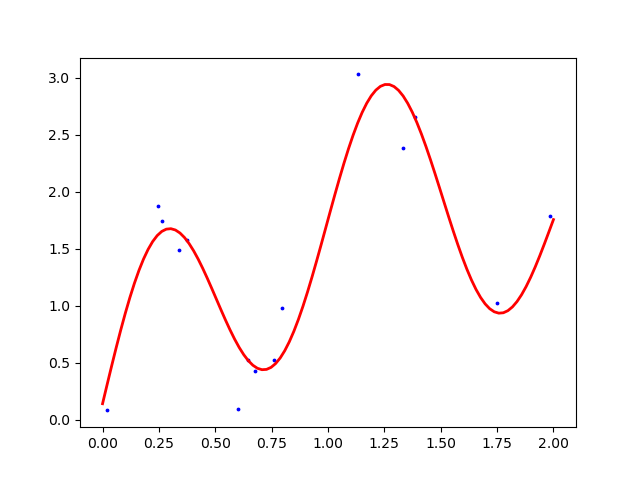
\includegraphics[scale=0.4]{polynomial_first/True_data.png}
\end{center}
It looks like a fifth degree polynomial fits this data the best, but how would we know what degree we should do at all? Let's just try fitting for different degree polynomials. 
\begin{figure}[hbt!]
    \centering 
    \begin{subfigure}[b]{0.32\textwidth}
    \centering
        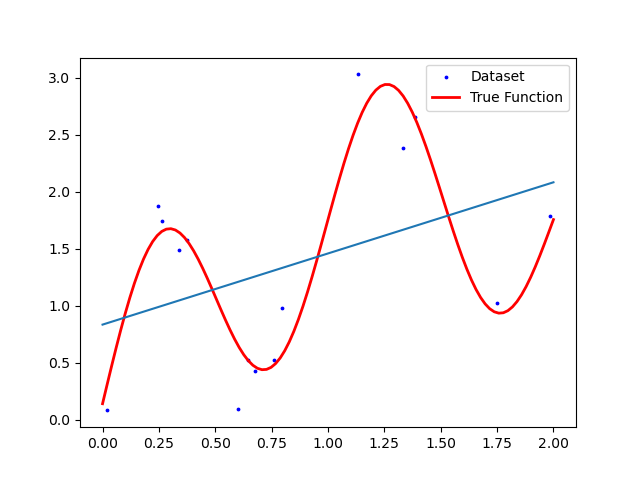
\includegraphics[width=\textwidth]{polynomial_first/poly_1_fit.png}
        \caption{1st Degree}
        \label{fig:1d}
    \end{subfigure}
    \hfill 
    \begin{subfigure}[b]{0.32\textwidth}
    \centering
        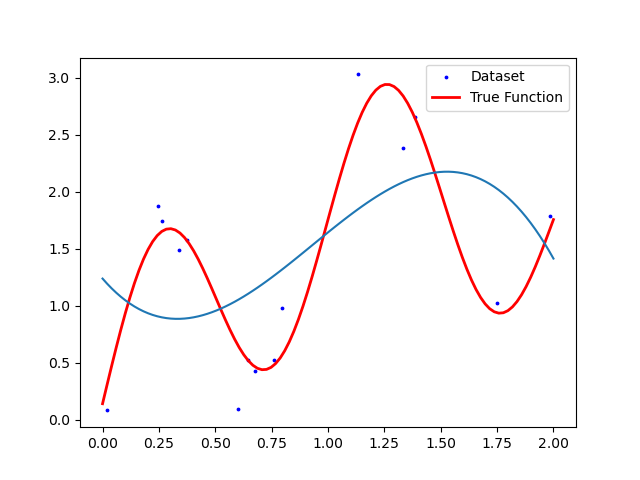
\includegraphics[width=\textwidth]{polynomial_first/poly_3_fit.png}
        \caption{3rd Degree}
        \label{fig:3d}
    \end{subfigure}
    \hfill 
    \begin{subfigure}[b]{0.32\textwidth}
    \centering
        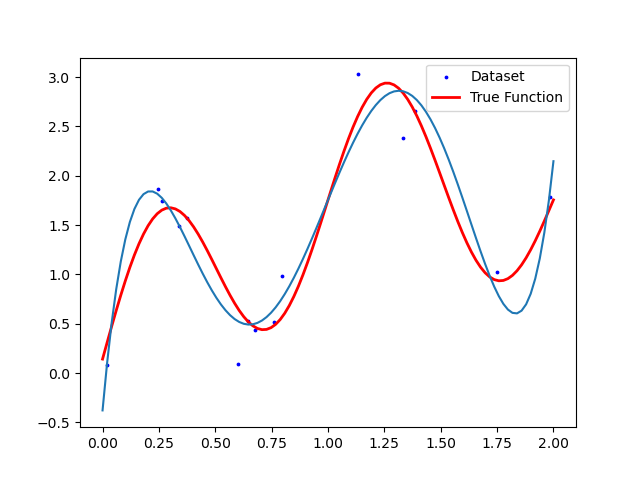
\includegraphics[width=\textwidth]{polynomial_first/poly_5_fit.png}
        \caption{5th Degree}
        \label{fig:5e}
    \end{subfigure}

    
    \begin{subfigure}[b]{0.32\textwidth}
    \centering
        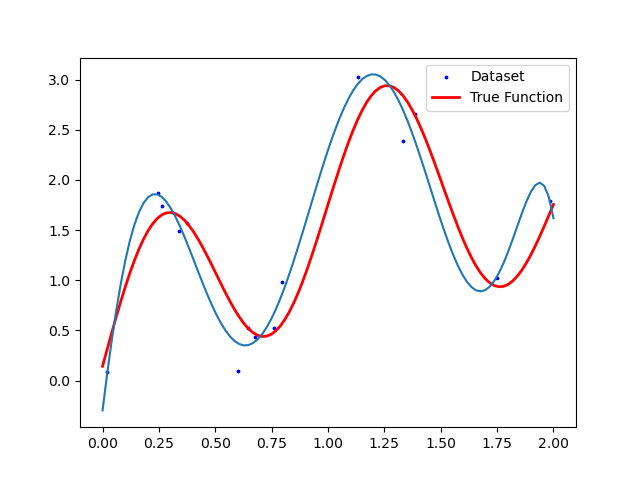
\includegraphics[width=\textwidth]{polynomial_first/poly_7_fit.png}
        \caption{7th Degree}
        \label{fig:7d}
    \end{subfigure}
    \hfill 
    \begin{subfigure}[b]{0.32\textwidth}
    \centering
        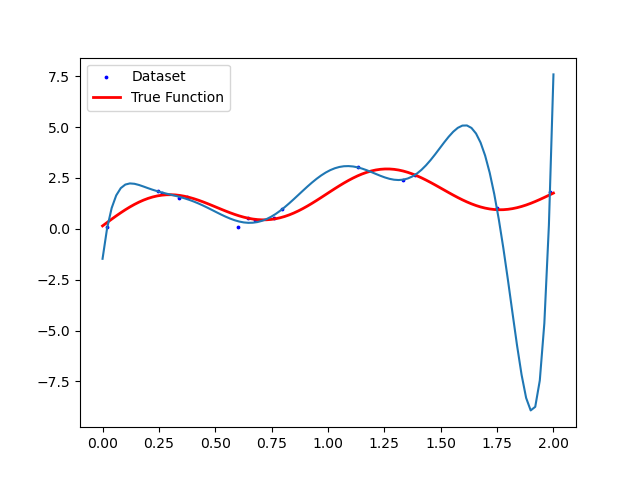
\includegraphics[width=\textwidth]{polynomial_first/poly_9_fit.png}
        \caption{9th Degree}
        \label{fig:9d}
    \end{subfigure}
    \hfill 
    \begin{subfigure}[b]{0.32\textwidth}
    \centering
        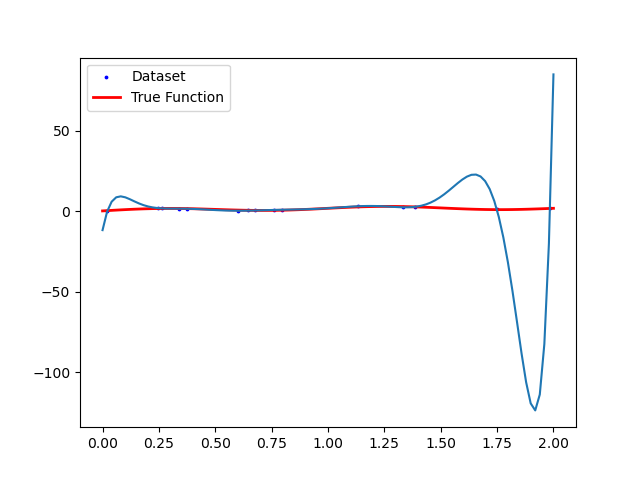
\includegraphics[width=\textwidth]{polynomial_first/poly_11_fit.png}
        \caption{11th Degree}
        \label{fig:11e}
    \end{subfigure}
\end{figure}

We already know that the 5th degree approximation is most optimal, and the lower degree ones are \textbf{underfitting} the data, while the higher degree ones are \textbf{overfitting}. As mentioned before, we can describe the underfitting and overfitting phenomena through the bias variance decomposition. 
\begin{enumerate}
    \item If we underfit the data, this means that our model is not robust and does not capture the patterns inherent in the data. It has a high bias since the set of function it encapsulates is not large enough to model $\mathbb{E}[Y\mid X]$. However, it has a low variance since if we were to take different samples of the dataset $\mathcal{D}$, the optimal parameters would not fluctuate. 

    \item What overfitting essentially means is that our model is too complex to the point where it starts to fit to the \textit{noise} of the data. This means that the variance is high, since different samples of the dataset $\mathcal{D}$ would cause huge fluctuations in the optimal trained parameters $\boldsymbol{\theta}$. However, the function set would be large, and thus it would be close to $\mathbb{E}[Y \mid X]$, leading to a low bias. 
\end{enumerate}

Another way to reduce the overfitting problem is if we have more training data to work with. That is, if we were to fit a 9th degree polynomial on a training set of not $N = 15$, but $N = 100$ data points, then we can see that this gives a much better fit. This makes sense because now the random variable $\mathcal{D}$, as a function of more random variables, has lower variance. Therefore, the lower variance in the dataset translates to lower variance in the optimal parameter. 
\begin{figure}[hbt!]
    \centering
    \begin{subfigure}[b]{0.48\textwidth}
    \centering
        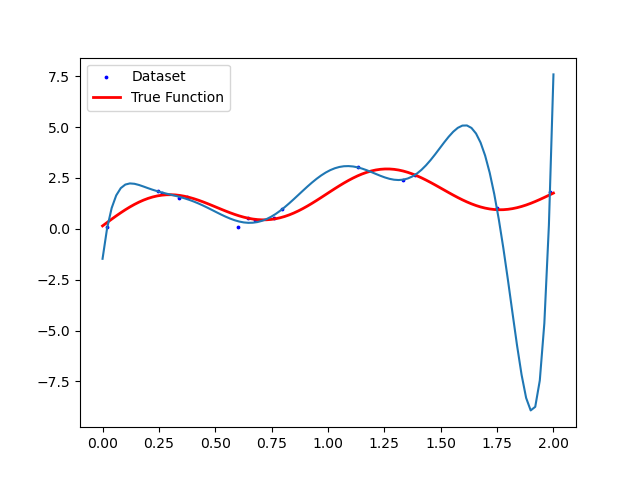
\includegraphics[width=\textwidth]{polynomial_first/poly_9_fit.png}
        \caption{$M = 9, N = 15$}
        \label{fig:d}
    \end{subfigure}
    \hfill 
    \begin{subfigure}[b]{0.48\textwidth}
    \centering
        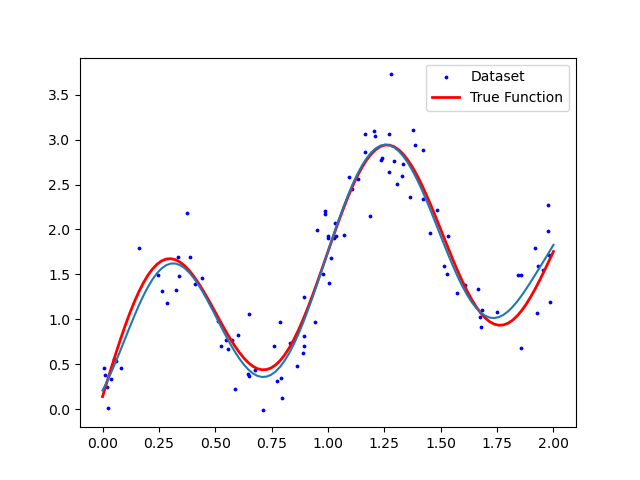
\includegraphics[width=\textwidth]{polynomial_first/increased_data.png}
        \caption{$M = 9, N = 100$}
        \label{fig:d}
    \end{subfigure}
    \caption{Increasing the number of data points helps the overfitting problem. Now, we can afford to fit a 9th degree polynomial with reasonable accuracy.}
\end{figure}

\subsubsection{Train Test Split and Cross Validation}

We have understood the theoretical foundations of overfitting and underfitting with the bias variance decomposition. But in practice, we don't have an ensemble of datasets; we just have one. Therefore, we don't actually know what the bias, the variance, or the noise is at all. Therefore, how do we actually \textit{know} in practice when we are underfitting or overfitting? Easy. We just split our dataset into 2 different parts: the training set and testing sets. 
\[\mathcal{D} = \mathcal{D}_{train} \sqcup \mathcal{D}_{test}\]

What we usually have is a \textbf{training set} that allows us to train the model, and then to check its performance we have a \textbf{test set}. We would train the model on the training set, where we will always minimize the loss, and then we would look at the loss on the test set. Though we haven't made a testing set, since we know the true model let us just generate more data and use that as our testing set. For each model, we can calculate the optimal $\boldsymbol{\theta}$, which we will denote $\boldsymbol{\theta}^\ast$, according to the \textbf{root mean squared loss}
\[h_{\boldsymbol{\theta}^\ast} = \argmin_{h_{\boldsymbol{\theta}}} \sqrt{ \frac{1}{N} \sum_{i=1}^N \big( y^{(i)} - h_{\boldsymbol{\theta}} (\mathbf{x}^{(i)}) \big)^2 }\]
where division of $N$ allows us to compare different sizes of datasets on equal footing, and the square root ensures that this is scaled correctly. Let us see how well these different order models perform on a separate set of data generated by the same function with Gaussian noise. 
\begin{figure}[hbt!]
    \centering
    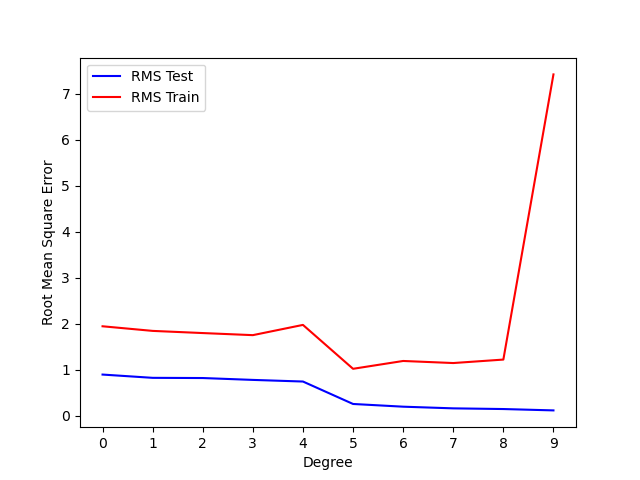
\includegraphics[scale=0.4]{polynomial_first/Degree_vs_RMS.png}
    \caption{Degree of Polynomial vs RMS on Training and Testing Sets}
    \label{fig:poly_deg_vs_rms}
\end{figure}
In $\ref{fig:poly_deg_vs_rms}$, we can see that the RMS decreases monotonically on the training error as more complex functions become more fine-tuned to the data. However, when we have a $9$th degree polynomial the RMS for the testing set dramatically increases, meaning that this model does not predict the testing set well, and performance drops. 


Now we know that a more complex model (i.e. that captures a greater set of functions) is not necessarily the best due to overfitting. Therefore, researchers perform \textbf{cross-validation} by taking the training set $(\mathcal{X}, \mathcal{Y})$. We divide it into $S$ equal pieces 
\[\bigcup_{s=1}^S D_s = (\mathcal{X}, \mathcal{Y})\]
Then, we train the model $\mathcal{M}$ on $S-1$ pieces of the data and then test it across the final piece, and do this $S$ times for every test piece, averaging its perforance across all $S$ test runs. Therefore, for every model $\mathcal{M}_k$, we must train it $S$ times, for all $K$ models, requiring $KS$ training runs. If data is particularly scarce, we set $S = N$, called the \textbf{leave-one-out} technique. Then we just choose the model with the best average test performance. 

To implement this in scikit-learn, we want to use the \texttt{train\_test\_split} class. We can also set a random state parameter to reproduce results. 
\begin{cverbatim}
from sklearn.model_selection import train_test_split 

# Split into training (80\%) and test (20\%) data 
X_train, X_test, Y_train, Y_test = train_test_split(X, Y, test_size=0.2, 
                                                    random_state=66)
\end{cverbatim}

However, this process requires a lot of training runs and therefore may be computationally infeasible. Therefore, various \textbf{information criterion} has been proposed to efficiently select a model. 


\subsubsection{Regularization}

So far, there are 2 ways to reduce the overfitting problem, either the decrease the model complexity or get more training data. A third way is to use a \textbf{regularizing} term, which adds a penalty term to the error function in order to discourage the coefficients from reaching large values. The two most popular ones are \textbf{ridge regression} 
\[E(\boldsymbol{\theta}) \coloneqq \frac{1}{2} \sum_{n=1}^N \big( h_{\boldsymbol{\theta}} (x^{(n)}) - y^{(n)} \big)^2 + \frac{\lambda}{2} ||\boldsymbol{\theta}||_2^2\]
which involves using the L2 norm of $\boldsymbol{\theta}$ and \textbf{LASSO regression} 
\[E(\boldsymbol{\theta}) \coloneqq \frac{1}{2} \sum_{n=1}^N \big( h_{\boldsymbol{\theta}} (x^{(n)}) - y^{(n)} \big)^2 + \frac{\lambda}{2} |\boldsymbol{\theta}|_1\]
which uses the L1 norm. These models are known as \textbf{shrinkage models}. We can add this term for the degree $M=9$ polynomial. 
\begin{figure}[hbt!]
    \centering
    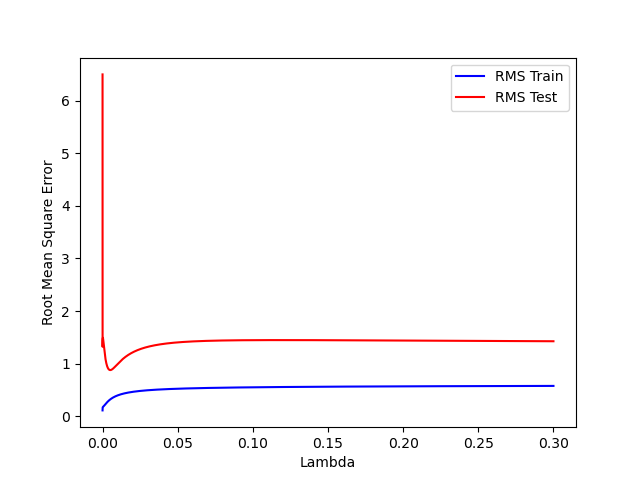
\includegraphics[scale=0.5]{polynomial_first/Lambda_vs_RMS.png}
    \caption{Even with a slight increase in the regularization term $\lambda$, the RMS error on the testing set heavily decreases. }
    \label{fig:enter-label}
\end{figure}

Now we can also add a regularization term in order to control overfitting, of the form $E(\boldsymbol{\theta}) = E_D (\boldsymbol{\theta}) + \lambda E_W (\boldsymbol{\theta})$. $E_W$ is a monotonically increasing function of some norm of $\boldsymbol{\theta}$ and so if $||\boldsymbol{\theta}||_q$ is big, then it penalizes the model more. Here we discuss 3 types of regularizers and the difference between them. 
\begin{enumerate}
    \item The ridge regularizer $E_W (\boldsymbol{\theta}) = \frac{1}{2} ||\boldsymbol{\theta}||_2^2$ can be imagined as drawing equipotential circles in $\mathcal{W}$. 

    \item The LASSO regularizer $E_W (\boldsymbol{\theta}) = \frac{1}{2} ||\boldsymbol{\theta}||_1 = \frac{1}{2} \sum_{j=1}^M |\theta_j|$ draws a diamond in the parameter space $\mathcal{W}$. This tends to give a sparser solution since the error function $E_D$ is more likely to ``touch" the corners of the contour plots of $E_W$. 

    \item The elastic net is a linear combination of the ridge and LASSO: $E_W (\boldsymbol{\theta}) = \lambda_2 ||\boldsymbol{\theta}||_2^2 + \lambda_1 ||\boldsymbol{\theta}||_1$. 
\end{enumerate}
Therefore, we can effectively limit the model complexity by adding a regularization to our error function so we don't have to worry about the number of basis functions $M$ to choose, but this now raises the question of how to determine a suitable regularization parameter $\lambda$. 
\begin{center}
    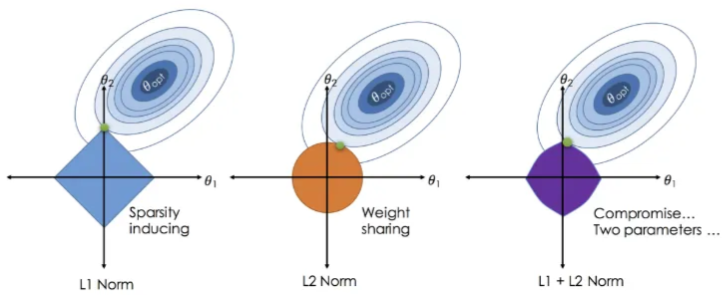
\includegraphics[scale=0.5]{Section_2/regularizers.png}
\end{center}

We can perform ridge, lasso, and elastic net regression very easily in sklearn, as such: 
\begin{cverbatim}
from sklearn.linear_model import Ridge, Lasso, ElasticNet
model1 = Ridge(alpha=0.1).fit(X, Y) 
model2 = Lasso(alpha=0.01).fit(X, Y)

# l1_ratio determines the balance between L1 and L2 regression
model3 = ElasticNet(alpha=0.5, l1_ratio=0.5) 
\end{cverbatim}

\subsubsection{Ensemble Learning}

The bias variance noise decomposition gives us a very nice way of explaining overfittting. That is, the bias (expectation of the squared difference between the true $\mathbb{E}[Y \mid X]$ and the expected trained hypothesis function $h_{\boldsymbol{\theta}; \mathcal{D}}$) reduces, but the variance in this overfitted model increases. Therefore, if we had a slightly different dataset $\mathcal{D}$ sampled from $(X \times Y)^N$, then we might have a very different trained hypothesis since it's so sensitive to the data. 

A way to treat this is through \textbf{ensemble learning}, where we train \textit{multiple} models over slightly different datasets, and then average their predictions in order to decrease the variance. Even though each model is trained over a smaller dataset, resulting it being more noisy, the average of all these slightly more noisy models will hopefully bring down the variance more than what we have added. There are two similar techniques: bagging and bootstrapping. 

\begin{definition}[Bootstrap Aggregating]
Given a dataset $\mathcal{D}$ of $N$ samples and a model $\mathcal{M}$, \textbf{bagging} is an ensemble method done with two steps: 
\begin{enumerate}
    \item Sample $\Tilde{N}$ data points with replacement from $\mathcal{D}$ to get a dataset $\mathcal{D}_1$, and do this $M$ times to get 
    \[\mathcal{D}_1, \mathcal{D}_2, \ldots, \mathcal{D}_M \subset \mathcal{D}\]
    \item For each sub dataset $\mathcal{D}_m$, train our model to get the optimal hypothesis $h_{\mathcal{D}_m}^\ast$. We should have $M$ different hypothesis functions, each trained on each sub dataset. 
    \[h_{\mathcal{D}_1}^\ast, h_{\mathcal{D}_2}^\ast, \ldots, h_{\mathcal{D}_M}^\ast\]
\end{enumerate}
To predict the output on a new value $\hat{\mathbf{x}}$, we can evaluate all the $h_{\mathcal{D}_m}^\ast (\hat{\mathbf{x}})$ .
\end{definition}

Let's


\subsection{Preprocessing Data}

\subsubsection{Feature Extraction}

The simplest linear function for regression is simply 
\[h_\mathbf{w} (\mathbf{x}) = w_0 + w_1 x_1 + \ldots + w_D x_D\]
This is called linear regression not because $h$ is a linear function of $\mathbf{x}$. It is a linear function of $\mathbf{w}$. Therefore, we can fix nonlinear functions $\phi_j (\mathbf{x})$ and consider linear combinations of them. 
\[h_\mathbf{w} (\mathbf{x}) = w_0 + \sum_{j=1}^{M-1} w_j \phi_j (\mathbf{x})\]
We usually choose a dummy basis function $\phi_0 (\mathbf{x}) = 1$ for notational convenience, so that if $\boldsymbol{\phi}$ is the vector of the function $\phi_j$, then we can write $h_\mathbf{w} (\mathbf{x}) = \mathbf{w}^T \boldsymbol{\phi} (\mathbf{x})$. This mapping from the original variables $\mathbf{x} \in \mathbb{R}^D$ to the basis functions $\{\phi_j (\mathbf{x})\}$, which span a linear function space of dimension $M$, is called \textbf{preprocessing} or \textbf{feature extraction} of the data. 

\begin{example}
Here are some examples of how we can extract features. 
\begin{enumerate}
    \item The mapping from a single variable $x$ to its powers 
    \[x \mapsto (1, x, x^2, \ldots, x^{M-1})\]

    \item The mapping from a configuration of $K$ atoms with their momenta in $\mathbb{R}^{6K}$ to their atomic cluster expansion polynomials. 

    \item The legendre polynomials, which form an orthonormal basis in the space of polynomials. 

    \item Using equally spaced Gaussian basis functions over the dataset as shown in Figure \ref{fig:Gaussian_basis_functions}. 
    \begin{figure}
        \centering
        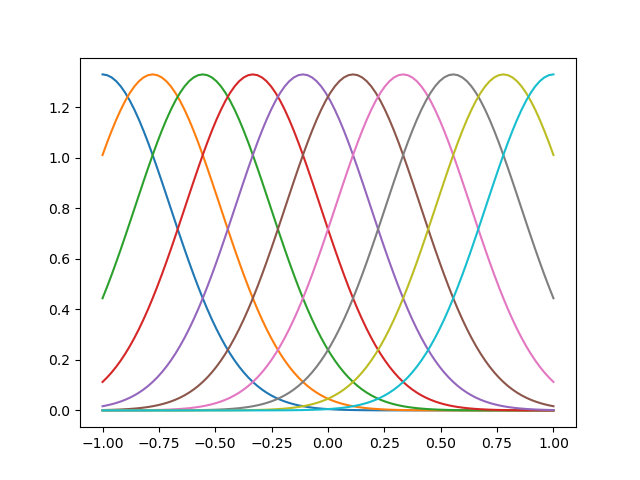
\includegraphics[scale=0.5]{Section_2/Gaussian_basis_functions.png}
        \caption{Gaussian basis functions over the interval $[-1, 1]$ with standard deviation of $0.3$}
        \label{fig:Gaussian_basis_functions}
    \end{figure}
\end{enumerate}
\end{example}

Changing the input space from $D$ dimensions to $M$ dimensions (i.e. extracting our $M$ features) gives the design matrix 
\[\mathbf{X} = \begin{pmatrix} \mathbf{x}^{(1)} \\ \mathbf{x}^{(2)} \\ \mathbf{x}^{(3)} \\ \vdots \\ \mathbf{x}^{(n)} \end{pmatrix} \implies \boldsymbol{\Phi} = \begin{pmatrix}
\text{---} & \phi(\mathbf{x}^{(1)}) & \text{---} \\
\text{---} & \phi(\mathbf{x}^{(2)}) & \text{---} \\
\vdots & \vdots & \vdots \\
\text{---} & \phi(\mathbf{x}^{(n)}) & \text{---}
\end{pmatrix}\]

We have shown that the $\texttt{PolynomialFeatures}$ transformer converts our features to a polynomial basis. We can do this for an arbitrary number of features, for example if we map $D = 2$ to a second degree polynomial, we would have the transformation 
\[(x_1, x_2) \mapsto (1, x_1, x_2, x_1^2, x_1 x_2, x_2^2)\]
\begin{cverbatim}
>>> import numpy as np
>>> from sklearn.preprocessing import PolynomialFeatures
>>> X = np.arange(6).reshape(3, 2)
>>> X
array([[0, 1],
       [2, 3],
       [4, 5]])
>>> poly = PolynomialFeatures(2)
>>> poly.fit_transform(X)
array([[ 1.,  0.,  1.,  0.,  0.,  1.],
       [ 1.,  2.,  3.,  4.,  6.,  9.],
       [ 1.,  4.,  5., 16., 20., 25.]])
\end{cverbatim}
Sometimes, we are only worried about the interaction terms among features, so we can set the parameter \texttt{interaction\_only=True}, which would, in the third degree case, transform the features 
\[(x_1, x_2, x_3) \mapsto (1, x_1, x_2, x_3, x_1 x_2, x_1 x_3, x_2 x_3, x_1 x_2 x_3)\]
\textbf{Spline transformers} are piecewise polynomials, which is also built in. We notice that it is cumbersome to transform the dataset \texttt{X} with the transformer, store it into another variable, and train the model on that. We can ``combine" the transforming (even multiple layers of transformers) and the model by implementing a ``pipeline," which is initialized by inputting a list of tuples (name and the object) and has the same methods as the model. 
\begin{cverbatim}
from sklearn.pipeline import Pipeline
model = Pipeline([("poly_transform", PolynomialFeatures(degree=2)), 
                  ("lin_regression", LinearRegression())
                  ]) 
model.fit(X, y)
\end{cverbatim}
Now, let's talk about how we can implement a custom transformer. We basically have to create a new subclass that implements the \texttt{fit} (which always returns \texttt{self}) and the \texttt{transform} (which returns the transformed matrix) methods. Here we show for Gaussian basis functions. 
\begin{cverbatim}
from sklearn.base import BaseEstimator, TransformerMixin

class GaussianFeatures(BaseEstimator, TransformerMixin):
    """Uniformly spaced Gaussian features for one-dimensional input"""
    
    def __init__(self, N, width_factor=2.0):
        self.N = N
        self.width_factor = width_factor
        
    def fit(self, X, y=None):
        # create N centers spread along the data range
        self.centers_ = np.linspace(X.min(), X.max(), self.N)
        self.width_ = self.width_factor * (self.centers_[1] - self.centers_[0])
        return self
        
    def transform(self, X): 
        transformed_rows = []
        for mu in self.centers_: 
            transformed_rows.append(stats.norm.pdf(X, mu, self.width_))
        
        return np.hstack(tuple(transformed_rows))

model = Pipeline([("gauss_transform", GaussianFeatures(20)), 
                  ("lin_regression", LinearRegression())
                  ]) 

N = 60
X = np.random.uniform(-1, 1, size=(N, 1)) 
Y = true_func(X) + np.random.normal(0, 0.3, size=(N, 1)) 

model = Pipeline([("gauss_transform", GaussianFeatures(10)), 
              ("lin_regression", LinearRegression())
              ]) 
model.fit(X, Y)
\end{cverbatim} 
If we would like to impelment the fourier expansion of a function of form 
\[f(x) = \frac{1}{2} a_0 + \sum_{n=1}^N a_n \cos(n x) + \sum_{n=1}^N b_n \sin(n x)\]
Then we would create the basis functions according to 
\begin{cverbatim}
class FourierFeatures(BaseEstimator, TransformerMixin): 
    "Fourier Expansion for one-dimensional input"
    
    def __init__(self, N): 
        self.N = N 
        
    def fit(self, X, Y=None): 
        return self
    
    def transform(self, X): 
        transformed_columns = [] 
        transformed_columns.append(np.ones(shape=X.shape))
        
        for n in range(self.N): 
            transformed_columns.append(np.sin(n * X))
            transformed_columns.append(np.cos(n * X))
            
        print(np.hstack(tuple(transformed_columns)).shape)
        return np.hstack(tuple(transformed_columns))
\end{cverbatim} 
and both of them would give the following fits to our original function $f(x) = \sin(2\pi x) + 2 \cos(x - 1.5)$. 
\begin{figure}[hbt!]
    \centering
    \begin{subfigure}[b]{0.48\textwidth}
    \centering
        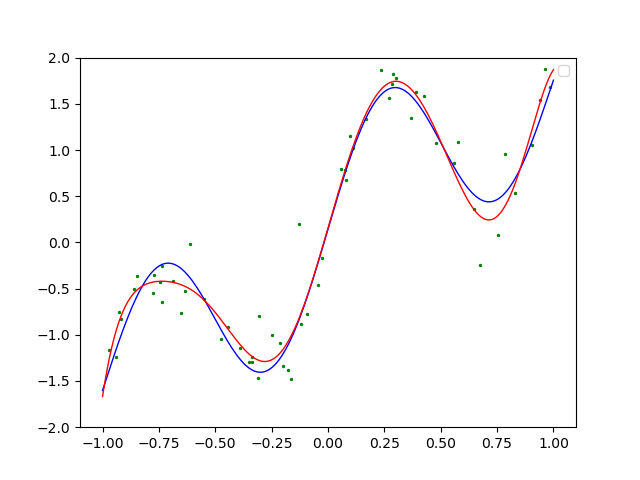
\includegraphics[width=\textwidth]{Section_2/Gaussian_Fit.png}
        \caption{Fitting with 10 Gaussian basis functions. }
        \label{fig:d}
    \end{subfigure}
    \hfill 
    \begin{subfigure}[b]{0.48\textwidth}
    \centering
        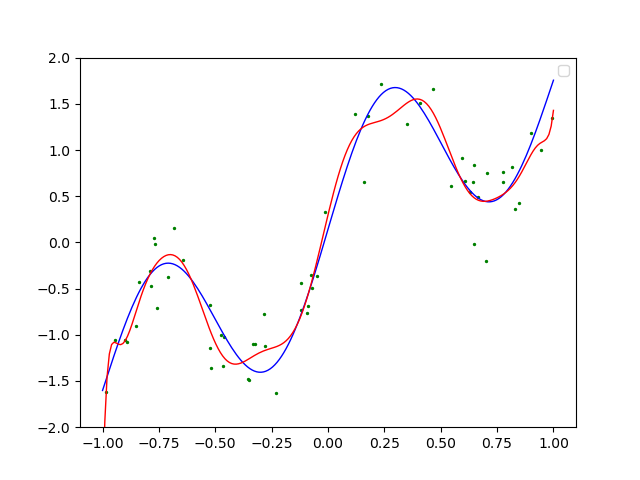
\includegraphics[width=\textwidth]{Section_2/Fourier_Fit.png}
        \caption{Fitting with 10 Fourier basis functions. }
        \label{fig:d}
    \end{subfigure}
    \caption{}
    \label{Coincide_mean}
\end{figure}


\subsubsection{Standardizing Data}

\textbf{Standardizing} typically meanss that our featuers will be rescaled to have the properties of a standard normal distribution with mean of $0$ and a standard deviation of $1$. Here are a few methods to scale our data, with their results shown on a dataset of $30$ points in $\mathbb{R}^2$. 
\begin{enumerate}
    \item \textbf{StandardScaler}: This is probably the most used method for standardizing data. It standardizes features by removing the mean and scaling to unit variance. The standard score of a sample $x^{(n)}$ is $(x - \bar{x})/S$ where $\bar{x}$ is the mean of the training samples and $S$ is the standard deviation of the training samples. 
    \begin{cverbatim}
    from sklearn.preprocessing import StandardScaler
    scaler = StandardScaler()
    scaled_data = scaler.fit_transform(data)
    \end{cverbatim}

    \item \textbf{MinMaxScaler}: While not technically "standardization," MinMaxScaler is another preprocessing method for scaling. It transforms features by scaling each feature to a given range, typically between zero and one, or so that the maximum absolute value of each feature is scaled to unit size. 
    \begin{cverbatim}
    from sklearn.preprocessing import MinMaxScaler
    scaler = MinMaxScaler()
    scaled_data = scaler.fit_transform(data)
    \end{cverbatim}

    \item \textbf{MaxAbsScaler}: This scaler works similarly to the MinMaxScaler but scales in a way that the training data lies within the range $[-1, 1]$ by dividing through the largest maximum value in absolute value. It is meant for data that is already centered at zero or sparse data. 
    \begin{cverbatim}
    from sklearn.preprocessing import MaxAbsScaler
    scaler = MaxAbsScaler()
    scaled_data = scaler.fit_transform(data)
    \end{cverbatim}

    \item \textbf{RobustScaler}: This scaler removes the median and scales the data according to the quantile range (defaults to IQR: Interquartile Range). It's robust to outliers, which makes it a good choice if you have data with possible outliers. 
    \begin{cverbatim}
    from sklearn.preprocessing import RobustScaler
    scaler = RobustScaler()
    scaled_data = scaler.fit_transform(data)
    \end{cverbatim} 

    \item \textbf{QuantileTransformer}: Note that the presence of outliers messes with our scaling. More generally for skewed distributions (like an exponential), a linear transformation does not take care of these outliers, so we would like some nonlinear preprocessing algorithm. One common one is the QuantileTransformer, which takes the quantiles (percentiles) of the dataset and transforms then so that those are equidistant from each other. By default, it divides up the data into 1000 quantiles. 
    \begin{cverbatim}
    from sklearn.preprocessing import QuantileTransformer
    transformer = QuantileTransformer(n_quantiles = 100, output_distribution='normal')
    transformed_data = transformer.fit_transform(data)
    \end{cverbatim}
\end{enumerate}

Let's talk about how these scalers will work on some data. We take a wine data with the two variables representing fixed acidity and volatile acidity. 
\begin{figure}[hbt!]
        \centering
        \begin{subfigure}[b]{0.32\textwidth}
        \centering
            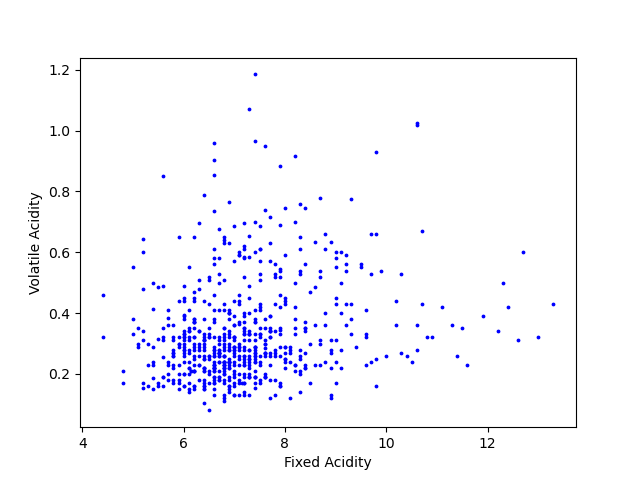
\includegraphics[width=\textwidth]{Standardize/Standard_scaler1.png}
            \caption{Original Data}
            \label{fig:d}
        \end{subfigure}
        \hfill
        \begin{subfigure}[b]{0.32\textwidth}
        \centering
            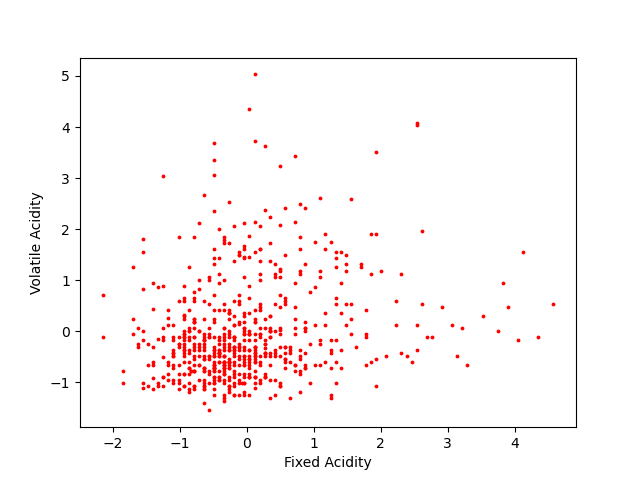
\includegraphics[width=\textwidth]{Standardize/Standard_scaler2.png}
            \caption{StandardScaler}
            \label{fig:d}
        \end{subfigure}
        \hfill
        \begin{subfigure}[b]{0.32\textwidth}
        \centering
            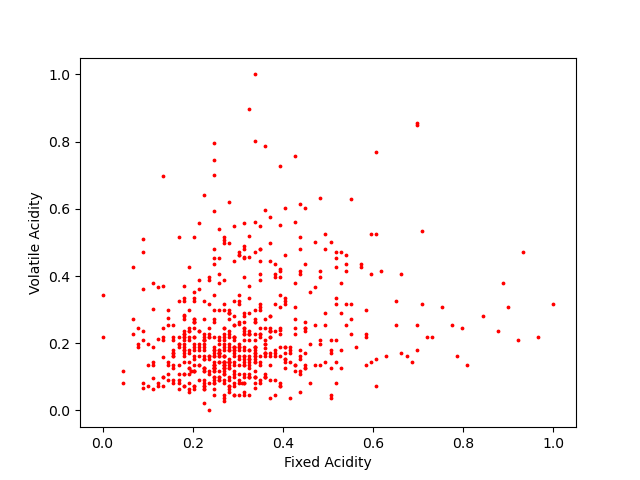
\includegraphics[width=\textwidth]{Standardize/MinMax_Scaler.png}
            \caption{MinMaxScaler}
            \label{fig:d}
        \end{subfigure}

        \begin{subfigure}[b]{0.32\textwidth}
        \centering
            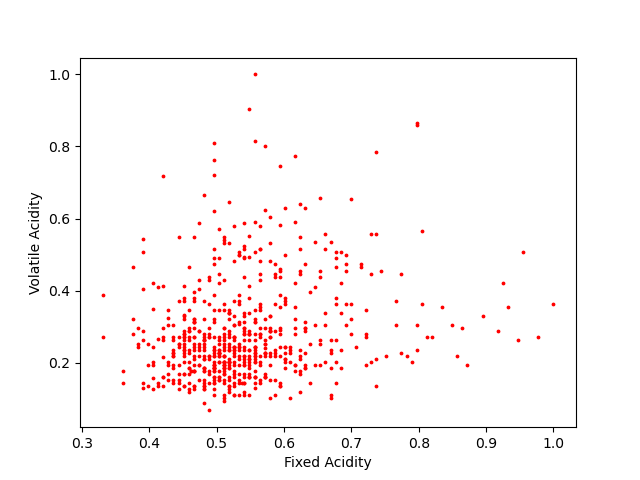
\includegraphics[width=\textwidth]{Standardize/MaxAbs_Scaler.png}
            \caption{MaxAbsScaler}
            \label{fig:d}
        \end{subfigure}
        \hfill
        \begin{subfigure}[b]{0.32\textwidth}
        \centering
            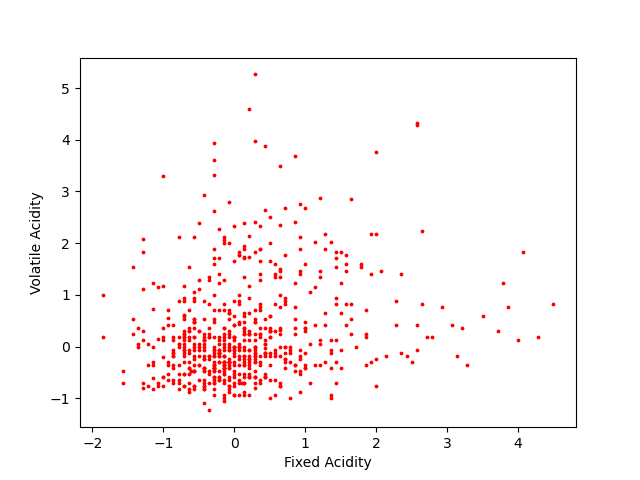
\includegraphics[width=\textwidth]{Standardize/Robust_Scaler.png}
            \caption{RobustScaler}
            \label{fig:d}
        \end{subfigure}
        \hfill
        \begin{subfigure}[b]{0.32\textwidth}
        \centering
            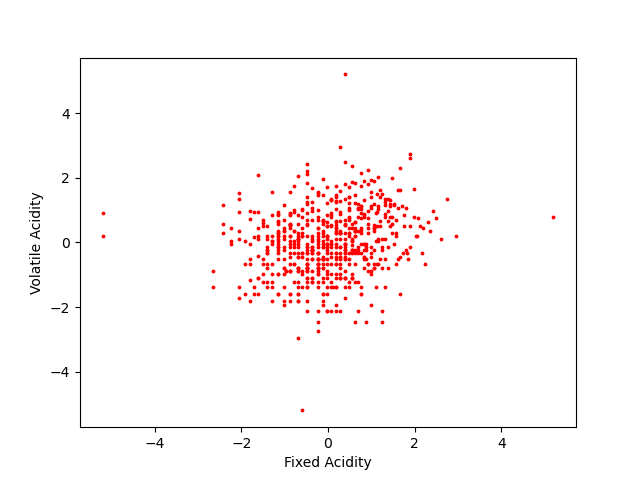
\includegraphics[width=\textwidth]{Standardize/Quantile_Scaler.png}
            \caption{QuantileTransformer}
            \label{fig:d}
        \end{subfigure}
        
        \caption{The StandardScaler simply standardizes the data to have $0$ mean and unit variance.}
        \label{Scalers}
    \end{figure}

It's important to note that whether you should standardize your data and how you should do it depends on the specific characteristics of your data and the machine learning algorithm you're using. For example, some algorithms, like many in deep learning, assume that all features are on the same scale. Others, like Decision Trees and Random Forests, do not require feature scaling at all. 


\subsection{Information Theory}

This final section does not relate directly to the workflow of training a machine learning model. Rather, it provides some very nice tools for us when analyzing the performance of these models. 

First, we want to quantitatively measure the ``surprise" of an event $E$ happening in a probability space by assigning it a value $I(E)$. We want it to satisfy the following: 
\begin{enumerate}
    \item $I(E) \geq 0$. The surprisal of any event is nonnegative. 
    \item $I(E) = 0$ iff $\mathbb{P}(E) = 1$. No surprisal is gained from events with probability $1$. 
    \item If $E_1$ and $E_2$ are independent events, then $I(E_1 \cap E_2) = I(E_1) + I(E_2)$. The information from two independent events should be the sum of their informations. 
    \item $I$ should be continuous, i.e. slight changes in probability correspond to slight changes in surprisal. 
\end{enumerate}

\begin{definition}[Surprisal]
Given a probability space $(\Omega, \mathcal{F}, \mathbb{P})$, the \textbf{surprisal}, or \textbf{self-information}, of an event $E \in \mathcal{F}$ is 
\[\sigma_\mathbb{P} (E) \coloneqq = - \log \mathbb{P}(E)\]
and the \textbf{expected surprisal} of $E$ is 
\[h_\mathbb{P} (E) = \mathbb{P}(E) \sigma_\mathbb{P} (E)\]
\end{definition}

Now we can define entropy as the expected surprisal of a random variable, which seems now more motivated and intuitive. 

\begin{definition}[Entropy]
Given a probability space $(\Omega, \mathcal{F}, \mathbb{P})$, a $\mathbb{P}$-almost partition is a set family $\mathcal{G} \subset \mathcal{F}$ such that $\mu(\cup_{G \in \mathcal{G}} G) = 1$ and $\mathbb{P}(A \cap B) = 0$ for all distinct $A, B \in \mathcal{G}$ (this is a relaxation of the usual conditions for a partition). The \textbf{entropy} of the subfamily $\mathcal{G}$ is 
\[H_\mathbb{P} (\mathcal{G}) \coloneqq \sum_{G \in \mathcal{G}} h_\mathbb{P}(G)\]
The \textbf{entropy} of the $\sigma$-algebra $\mathcal{F}$ is defined 
\[H_\mathbb{P} (\mathcal{F}) = \sup_{\mathcal{G} \subset \mathcal{F}} H_\mathbb{P} (\mathcal{G})\]
\end{definition}

\begin{example}
For a discrete random variable, since we are working with its power set, the entropy reduces to 
\[H[X] \coloneqq \mathbb{E}[-\ln{p(X)}] = -\sum_x \mathbb{P}(X = x) \ln{\mathbb{P}(X = x)}\]
\end{example}

Intuitively, this represents the element of surprise of a certain data point, and distributions that have relatively sharp peaks will have lower entropy (since we expect most of the samples to come from the peaks) while uniform distributions have higher entropy. The entropy also demonstrates the average length (if base is $2$) number of bits required to transmit the state of a random variable. 

\begin{definition}[Joint, Conditional Entropy]
We can define the joint entropy and conditional entropy between two discrete random variables $X, Y$ as 
\begin{align*}
    H(X, Y) & = \mathbb{E}_{X \times Y} [-\log \mathbb{P}(X = x, Y = y)] \\
    H(X \mid Y) & = \mathbb{E}[- \log \mathbb{P}(X = x \mid Y = y)]
\end{align*}
\end{definition}

\subsubsection{Kullback Leibler Divergence}

The \textbf{relative entropy}, or \textbf{Kullback-Leibler divergence}, of distributions $p(x)$ and $q(x)$ is defined 
\begin{align*}
    \mathrm{KL}(p || q) & \coloneqq - \int p(\mathbf{x}) \, \ln{q(\mathbf{x})} \,d\mathbf{x} - \bigg( - \int p(\mathbf{x}) \, \ln{p(\mathbf{x})} \,d\mathbf{x} \bigg) \\
    & = - \int p(\mathbf{x}) \, \ln \bigg( \frac{q(\mathbf{x})}{p(\mathbf{x})} \bigg) \,d\mathbf{x} 
\end{align*}
We can show that this quantity is always greater than or equal $0$ by Jensen's inequality using the fact that $-\ln(x)$ is concave
\[\int p(\mathbf{x}) \, -\ln \bigg( \frac{q(\mathbf{x})}{p(\mathbf{x})} \bigg) \,d\mathbf{x} \geq -\ln \int p(\mathbf{x}) \, \frac{q(\mathbf{x})}{p(\mathbf{x})} \,d\mathbf{x} = -\ln \int q(\mathbf{x}) \,d\mathbf{x} = -\ln(1) = 0\]
and it is precisely $0$ if $p = q$, so it behaves similarly to a metric. However, it isn't exactly since it is not symmetric. 

Let's demonstrate how entropy and the KL divergence applies to maximum likelihood estimation. Suppose that iid samples $\mathcal{D} = \{(x^{(n)}, y^{(n)}\}$ are given in a regression problem. Let $P^\ast = (X, Y)$ be the true data generating function. Then, we want to compute an approximation of $P^\ast$ with $P_\theta$, where $P_\theta$ is some parameterized distribution. The negative log likelihood of the $y$'s being generated is 
\[\ell(\theta) = \frac{1}{N} \sum_{n=1}^N \log P_\theta (y_i \mid x_i)\]
which asymptotically converges to 
\[\mathbb{E}_{P^\ast} [ -\log P_\theta (y_i \mid x_i)] = \mathrm{KL}(P^\ast || P) + H[P^\ast]\]
and since the entropy is constant, this is equivalent to minimizing the KL divergence between $P$ and $P^\ast$. 

We assume that the $y^{(n)}$'s come from a conditional distribution $P_{\theta, x_i}$, where the parameters of the distribution is $\theta$ and $x_i$ 


\subsubsection{Mutual Information}

\begin{definition}[Differential Entropy]
For a continuous random vector, the \textbf{differential entropy} is defined 
\[H[\mathbf{X}] = - \int p(\mathbf{x}) \ln{p(\mathbf{x})} \,d\mathbf{x}\]
\end{definition}

\begin{definition}[Mutual Information]
The \textbf{mutual information} between random variables $X, Y$ is the decrease in entropy when we condition $X$ by $Y$. 
\[I(X ; Y) = H(X) - H(X \mid Y) = H(Y) - H(Y \mid X)\]
This can be conditioned on another random variable $Z$. 
\[I(X ; Y \mid Z) = H(X \mid Z) - H(X \mid Y, Z) = H(Y \mid Z) - H(Y \mid X, Z)\]
\end{definition}



\section{Linear Regression}

\subsection{Construction}

Let $\beta$ be a matrix of parameters, and let $X$ be a vector of covariates. Then, for each observed $Y$, we make the following assumption 
\[Y = X \beta + \epsilon, \text{ where } \epsilon \sim N(\mathbf{0}, \sigma^2 I)\]

We have the following assumptions: 
\begin{enumerate}
  \item \textit{Weak exogeneity}: the covariates are observed without error.
  \item \textit{Linearity}: the mean of the variate is a linear combination of the parameters and the covariates.
  \item \textit{Constant variance}: call it homoscedasticity for bonus points on terminology (in contrast to heteroscedasticity).
  This means that all the observations of $Y$ are assumed to have the same, constant variance.
  \item \textit{Independence of errors}: we assume that the errors of the variates are uncorrelated.
  \item \textit{No multicollinearity}: more properly, the lack of perfect multicollinearity. Assume that the covariates aren't perfectly correlated. See discussion below.
  \item \textit{Errors have a statistical distribution}: this isn't strictly necessary, but it makes prediction theoretically coherent. The usual assumption is that the errors have a normal distribution, but others can also be used.
  (For instance, the t-distribution is used for ``robust regression'', where the variance observed is larger than that of the normal distribution.)
\end{enumerate}

In order to check multicollinearity, we compute the correlation matrix. 

\begin{definition}[Correlation Matrix]
The correlation matrix of random variables $X_1, \ldots, X_d$ is 
\[\mathbf{C}_{ij} = \Corr(X_i, X_j) = \frac{\Cov(X_i, X_j)}{\sigma_{X_i} \sigma_{X_j}}\]
given that $\sigma_{X_i} \sigma_{X_j} > 0$. Clearly, the diagonal entries are $1$, but if there are entries that are very close to $1$, then we have multicollinearity. 
\end{definition}

Assume that two variables are perfectly correlated. Then, there would be pairs of parameters that are indistinguishable if moved in a certain linear combination. This means that the variance of $\hat{\boldsymbol{\beta}}$ will be very ill conditioned, and you would get a huge standard error in some direction of the $\beta_i$'s. We can fix this by making sure that the data is not redundant and manually removing them, standardizing the variables, making a change of basis to remove the correlation, or just leaving the model as it is. 

If these assumptions don't hold, 
\begin{enumerate}
  \item \textit{Weak exogeneity}: the sensitivity of the model can be tested to the assumption of weak exogeneity by doing bootstrap sampling for the covariates and seeing how the sampling affects the parameter estimates.
  Covariates measured with error used to be a difficult problem to solve, as they required errors-in-variables models, which have very complicated likelihoods. In addition, there is no universal fitting library to deal with these. But nowadays, with the availability of Markov Chain Monte Carlo (MCMC) estimation through probabilistic programming languages, it is a lot easier to deal with these using Bayesian hierarchical models (or multilevel models, or Bayesian graphical models---these have many names).
  \item \textit{Linearity}: the linear regression model only assumes linearity in the parameters, not the covariates. Therefore you could build a regression using non-linear transformations of the covariates, for instance,
  \[
    Y = X_1 \beta_1 +
        X_1^2 \beta_2 +
        \log(X_1) \beta_3
    \text{.}
  \]
  If you need to further relax the assumption, you are better off using non-linear modelling. 
  \item \textit{Constant variance}: the simplest fix is to do a variance-stabilising transformation on the data. Assuming a constant coefficient of variation rather than a constant mean could also work. Some estimation libraries (such as the \verb+glm+ package in R) allow specifying the variance as a function of the mean.
  \item \textit{Independence of errors}: this is dangerous because in the financial world things are usually highly correlated in times of crisis. The most important thing is to understand how risky this assumption is for your setting. If necessary, add a correlation structure to your model, or do  a multivariate regression. Both of these require significant resources to estimate parameters, not only in terms of computational power but also in the amount of data required.
  \item \textit{No multicollinearity}:  
  if the covariates are correlated, they can still be used in the regression, but numerical problems might occur depending on how the fitting algorithms invert the matrices involved.
  The t-tests that the regression produces can no longer be trusted. All the covariates must be included regardless of what their significance tests say.
  A big problem with multicollinearity, however, is over-fitting.
  Depending on how bad the situation is, the parameter values might have huge uncertainties around them, and if you fit the model using new data their values might change significantly.
  I suggest reading the Wikipedia article on multicollinearity, as it contains useful information: \\
  \url{https://en.wikipedia.org/wiki/Multicollinearity} \\
  Multicollinearity is a favourite topic of discussion for interviewers, and they usually have strong opinions about how it should be handled.
  The model's intended use will determine how sensitive it is to ignoring the error distribution.
  In many cases, fitting a line using least-squares estimation is equivalent to assuming errors have a normal distribution.
  If the real distribution has heavier tails, like the t-distribution, how risky will it make decisions based on your outputs?
  One way to address this is to use a technique like robust-regression.
  Another way is to think about the dynamics behind the problem and which distribution would be best suited to model them---as opposed to just fitting a curve through a set of points.
\end{enumerate}

\subsection{Least Squares}

Given the design matrix $\mathbf{X}$, we can present the linear model in vectorized form: 
\[\mathbf{Y} = \mathbf{X} \boldsymbol{\beta} + \boldsymbol{\epsilon}, \; \boldsymbol{\epsilon} \sim N(\mathbf{0}, \sigma^2 \mathbf{I})\]
The errors can be written as $\boldsymbol{\epsilon} = \mathbf{Y} - \mathbf{X} \boldsymbol{\beta}$, and you have the following total sum of squared errors: 
\[S(\boldsymbol{\beta}) = \boldsymbol{\epsilon}^T \boldsymbol{\epsilon} = (\mathbf{Y} - \mathbf{X} \boldsymbol{\beta})^T (\mathbf{Y} - \mathbf{X} \boldsymbol{\beta})\]
We want to find the value of $\boldsymbol{\beta}$ that minimizes the sum of squared errors. In order to do this, remember the following matrix derivative rules when differentiating with respect to vector $\mathbf{x}$. 
\begin{enumerate}
    \item $\mathbf{x}^T \mathbf{A} \mapsto \mathbf{A}$
    \item $\mathbf{x}^T \mathbf{A} \mathbf{x} \mapsto 2 \mathbf{A} \mathbf{x}$
\end{enumerate}
Now this should be easy. 
\begin{align*}
    S(\boldsymbol{\beta}) & = \mathbf{Y}^T \mathbf{Y} - \boldsymbol{\beta}^T \mathbf{X}^T \mathbf{Y} - \mathbf{Y}^T \mathbf{X} \boldsymbol{\beta} + \boldsymbol{\beta}^T \mathbf{X}^T \mathbf{X} \boldsymbol{\beta} \\
    & = \mathbf{Y}^T \mathbf{Y} - 2 \mathbf{Y}^T \mathbf{X} \boldsymbol{\beta} + \boldsymbol{\beta}^T \mathbf{X}^T \mathbf{X} \boldsymbol{\beta} \\
    \frac{\partial}{\partial \boldsymbol{\beta}} S(\boldsymbol{\beta}) & = - 2 \mathbf{X}^T \mathbf{Y} + 2 \mathbf{X}^ \mathbf{X} \boldsymbol{\beta}
\end{align*}
and setting it to $\mathbf{0}$ gives 
\[2 \mathbf{X}^T \mathbf{X} \boldsymbol{\beta} - 2 \mathbf{X}^T \mathbf{Y} = 0 \implies \mathbf{X}^T \mathbf{X} \boldsymbol{\beta} = \mathbf{X}^T \mathbf{Y}\]
and the variance of $\boldsymbol{\beta}$, by using the fact that $\Var[\mathbf{A} \mathbf{X}] = \mathbf{A} \Var[X] \mathbf{A}^T$, is
\[\Var(\hat{\boldsymbol{\beta}}) =
 (\mathbf{X}^{\prime} \mathbf{X})^{-1} \mathbf{X}^{\prime}
 \;\sigma^2 \mathbf{I} \; \mathbf{X}  (\mathbf{X}^{\prime} \mathbf{X})^{-1}
= \sigma^2 (\mathbf{X}^{\prime} \mathbf{X})^{-1} (\mathbf{X}^{\prime}
 \mathbf{X})  (\mathbf{X}^{\prime} \mathbf{X})^{-1}
= \sigma^2  (\mathbf{X}^{\prime} \mathbf{X})^{-1}\]
But we don't know the true $\sigma^2$, so we estimate it with $\hat{\sigma}^2$ by taking the variance of the residuals. Therefore, we have 
\begin{align*}
    \boldsymbol{\beta} & = (\mathbf{X}^T \mathbf{X})^{-1} \mathbf{X}^T \mathbf{Y} \in \mathbb{R}^d \\
    \Var(\hat{\boldsymbol{\beta}}) & = \hat{\sigma}^2 (\mathbf{X}^T \mathbf{X})^{-1} \in \mathbb{R}^{d \times d}
\end{align*}

\begin{example}
What happens if you copy your data in OLS? In this case, our MLE estimate becomes 
\begin{align*}
    \left(\begin{pmatrix}X \\ X \end{pmatrix}^T \begin{pmatrix} X \\ X \end{pmatrix} \right )^{-1} & \begin{pmatrix} X \\ X  \end{pmatrix}^T \begin{pmatrix} Y \\ Y  \end{pmatrix}  =\\
& = (X^T X + X^T X)^{-1} (X^T Y + X^T Y ) = (2 X^T X)^{-1} 2 X^T Y = \hat{\beta}
\end{align*}
and our estimate is unaffected. However, the variance shrinks by a factor of $2$ to 
\[\frac{\sigma^2}{2} (\mathbf{X}^T \mathbf{X})^{-1}\]
A consequence of that is that confidence intervals will shrink with a factor of $1/\sqrt{2}$. The reason is that we have calculated as if we still had iid data, which is untrue. The pair of doubled values are obviously dependent and have a correlation of $1$. 
\end{example}

\subsection{Likelihood Estimation}

Given a dataset $\mathcal{D} = \{(x^{(i)}, y^{(i)})\}_{i=1}^N$, our likelihood is 
\[L(\theta ; \mathcal{D}) = \prod_{i=1}^N p(y^{(i)} \mid x^{(i)}; \theta) = \prod_{i=1}^N \frac{1}{\sqrt{2 \pi \sigma^2}} \exp \bigg( -\frac{(y^{(i)} - \theta^T x^{(i)})^2}{2 \sigma^2} \bigg)\]
We can take its negative log, remove additive constants, and scale accordingly to get 
\begin{align*}
    \ell (\theta) & = -\frac{N}{2} \ln{\sigma^2} - \frac{N}{2} \ln(2 \pi) + \frac{1}{2 \sigma^2} \sum_{i=1}^N \big(y^{(i)} - \boldsymbol{\theta}^T \mathbf{x}^{(i)} \big)^2 \\
    & =\frac{1}{2} \sum_{i=1}^N \big(y^{(i)} - \boldsymbol{\theta}^T \mathbf{x}^{(i)} \big)^2 
\end{align*}
which then corresponds to minimizing the sum of squares error function. Taking the gradient of this log likelihood w.r.t. $\theta$ gives 
\[\nabla_\theta \ell (\theta) = \sum_{i=1}^N ( y^{(i)} - \theta^T x^{(i)}) x^{(i)} \]
and running gradient descent over a minibatch $M \subset \mathcal{D}$ gives 
\begin{align*}
    \theta & = \theta - \eta \nabla_\theta \ell (\theta) \\
    & = \theta - \eta \sum_{(x, y) \in M} (y - \theta^T x) x
\end{align*}
This is guaranteed to converge since $\ell(\theta)$, as the sum of convex functions, is also convex. 

Note that since we can solve this in closed form, by setting the gradient to $0$, we have 
\[0 = \sum_{n=1}^N y^{(n)} \boldsymbol{\phi}(\mathbf{x}^{(n)})^T - \mathbf{w}^T \bigg( \sum_{n=1}^N \boldsymbol{\phi}(\mathbf{x}^{(n)}) \boldsymbol{\phi}(\mathbf{x}^{(n)})^T \bigg)\]
which is equivalent to solving the least squares equation 
\[\mathbf{w}_{ML} = ( \boldsymbol{\Phi}^T \boldsymbol{\Phi})^{-1} \boldsymbol{\Phi}^T \mathbf{Y}\]
Note that if we write out the bias term out explicitly, we can see that it just accounts for the translation (difference) between the average of the outputs $\bar{y} = \frac{1}{N} \sum_{n=1}^N y_n$ and the average of the basis functions $\bar{\phi_j} = \frac{1}{N} \sum_{n=1}^N \phi_j (\mathbf{x}^{(n)})$. 
\[w_0 = \bar{y} - \sum_{j=1}^{M-1} w_j \bar{\phi_j}\]
We can also maximize the log likelihood w.r.t. $\sigma^2$, which gives the MLE 
\[\sigma^2_{ML} = \frac{1}{N} \sum_{n=1}^N \big( y^{(n)} - \mathbf{w}^T_{ML} \boldsymbol{\phi}(\mathbf{x}^{(n)}) \big)^2\]

\subsection{Simple Linear Regression}

The simple linear regression is the special case of the linear regression with only one covariate. 
\[y = \alpha + x \beta\]
which is just a straight line fit. Interviewers like this model for its aesthetically pleasing theoretical properties. A few of them are described here, beginning with parameter estimation. For $n$ pairs of $(x_i, y_i)$, 
\[y_i = \alpha + \beta x_i + \epsilon_i\]
To minimize the sum of squared errors 
\[\sum_{i} \epsilon_i^2 = \sum_{i} (y_i - \alpha - \beta x_i)^2\]
Taking the partial derivatives w.r.t. $\alpha$ and $\beta$ and setting them equal to $0$ gives 
\begin{align*}
    &\sum_i (y_i - \hat{\alpha} - \hat{\beta} x_i) = 0 \\
    &\sum_i (y_i - \hat{\alpha} - \hat{\beta} x_i) x_i = 0
\end{align*}
From just the first equation, we can write 
\[n \bar{y} = n \hat{\alpha} + n \hat{\beta} \bar{x} \implies y = \hat{\alpha} + \hat{\beta} \bar{x} \implies \hat{\alpha}  = \bar{y} - \hat{\beta} \bar{x} \]
The second equation gives 
\[\sum_{i} x_i y_i = \hat{\alpha} n \bar{x} + \hat{\beta} \sum_{i} x_i^2\]
and substituting what we derived gives 
\begin{align*}
    \sum_{i} x_i y_i & = (\bar{y} - \hat{\beta} \bar{x}) n \bar{x} + \hat{\beta} \sum_i x_i^2 \\
    & = n \bar{x} \bar{y} + \hat{\beta} \bigg( \Big(\sum_i x_i^2 \Big) - n \bar{x}^2 \bigg)
\end{align*}
and so we have 
\[\hat{\beta} = \frac{ \big( \sum_i x_i y_i \big) - n \bar{x}\bar{y}}{\big( \sum x_i^2 \big) - n \bar{x}^2} = \frac{ \sum_i x_i y_i - \bar{x} y_i}{\sum x_i^2 - \bar{x} x_i} = \frac{ \sum_i (x_i - \bar{x}) y_i}{\sum_i (x_i - \bar{x}) x_i}\]
Now we can use the identity
\begin{align*}
    \sum_{i} (x_i - \bar{x}) (y_i - \bar{y}) & = \sum_i y_i (x_i - \bar{x}) = \sum_i x_i (y_i - \bar{y}) 
\end{align*}
to substitute both the numerator and denominator of the equation to 
\begin{align*}
    \hat{\beta} & = \frac{\sum_i (x_i - \bar{x}) (y_i - \bar{y})}{\sum_i (x_i - \bar{x})^2} = \frac{\mathrm{cov}(x, y)}{\mathrm{var}(x)} = \rho_{xy} \frac{s_y}{s_x}
\end{align*}
where $\rho_{xy}$ is the correlation between $x$ and $y$, and the variance and covariance represent the sample variance and covariance (indicated in lower case letters). Therefore, the correlation coefficient $\rho_{xy}$ is precisely equal to the slope of the best fit line when $x$ and $y$ have been standardized first, i.e. $s_x = s_y = 1$. 

\begin{example}
Say that we are fitting $Y$ onto $X$ in a simple regression setting with MLE $\beta_1$, and now we wish to fit $X$ onto $Y$. How will the MLE slope change? We can see that 
\[\beta_1 = \rho \frac{s_y}{s_x} , \;\; \beta_2 = \rho \frac{s_x}{s_y}\]
and so 
\[\beta_2 = \rho^2 \frac{1}{\rho} \frac{s_x}{s_y} = \rho^2 \frac{1}{\beta_1} = \beta_1 \frac{\mathrm{var}(x)}{\mathrm{var}(y)}\]
The reason for this is because regression lines don't necessarily correspond to one-to-one to a casual relationship. Rather, they relate more directly to a conditional probability or best prediction. 
\end{example}

The \textbf{coefficient of determination} $R^2$ is a measure tells you how well your line fits the data. When you have your $y_i$'s, their deviation around its mean is captured by the sample variance $s^2_y = \sum_i (y_i - \bar{y})^2$. When we fit our line, we want the deviation of $y_i$ around our predicted values $\hat{y}_i$, i.e. our sum of squared loss $\sum_i (y_i - \hat{y}_i)^2$, to be lower. Therefore, we can define 
\[R^2 = 1 - \frac{\mathrm{MSE Loss}}{\mathrm{var}(y)} = 1 - \frac{\sum_i (y_i - \hat{y}_i)^2}{\sum_i (y_i - \bar{y})^2}\]
In simple linear regression, we have 
\[R^2 = \rho_{yx}^2\]
An $R^2$ of $0$ means that the model does not improve prediction over the mean model and $1$ indicates perfect prediction. However, a drawback of $R^2$ is that it can increase if we add predictors to the regression model, leading to a possible overfitting. 

\begin{theorem}
The residual sum of squares (RSS) is equal to the a proportion of the variance of the $y_i$'s. 
\[\mathrm{RSS} = \sum (y_i - \hat{y}_i)^2 = (1 - \rho^2) \sum (y_i - \bar{y})^2 \]
\end{theorem}

\subsection{Significance Tests}

\subsubsection{T Test}

Given some multilinear regression problem where we must estimate $\boldsymbol{\beta} \in \mathbb{R}^{D + 1}$ ($D$ coefficients and $1$ bias), we must determine whether there is actually a linear relationship between the $x$ and $y$ variables in our dataset $\mathcal{D}$. Say that we have a sample of $N$ points $\mathcal{D} = \{(x_n, y_n)\}_{n=1}^N$. Then, for each ensemble of datasets $\mathcal{D}$ that we sample from the distribution $(X \times Y)^N$, we will have some estimator $\boldsymbol{\beta}$ for each of them. This will create a sampling distribution of $\boldsymbol{\beta}$'s where we can construct our significance test on. 

So what should our sampling distribution of $\hat{\boldsymbol{\beta}}$ be? It is clearly normal since it is just a transformation of the normally distributed $Y$: $\hat{\boldsymbol{\beta}} \sim N (\boldsymbol{\beta}, \sigma^2 (X^T X)^{-1})$. Therefore, only considering one element $\beta_i$ here, 
\[\frac{\hat{\beta}_i - \beta_i}{\sigma \sqrt{ (X^T X)^{-1}_{ii}}} \sim N(0, 1)\]
But the problem is that we don't know the true $\sigma^2$, and we are estimating it with $\hat{\sigma}^2$. If we knew the true $\sigma^2$ then this would be a normal, but because of this estimate, our normalizing factor is also random. It turns out that the residual sum of squares (RSS) for a multiple linear regression
\[\sum_{i} (y_i - x_i^T \beta)^2 \]
follows a $\chi^2_{n-d}$ distribution. Additionally from the $\chi^2$ distribution of RSS we have 
\[\frac{(n - d) \hat{\sigma}^2}{\sigma^2} \sim \chi^2_{n-d}\]
where we define $\hat{\sigma}^2 = \frac{\mathrm{RSS}}{n-d}$ which is an unbiased estimator for $\sigma^2$. Now there is a theorem that says that if you divide a $N(0, 1)$ distribution by a $\chi^2_k / k$ distribution (with $k$ degrees of freedom), then it gives you a $t$-distribution with the same degrees of freedom. Therefore, we divide 
\[\frac{\frac{\hat{\beta}_i - \beta_i}{\sqrt{ (X^T X)^{-1}_{ii}}}}{\hat{\sigma}} = \frac{ \sigma \sim N(0, 1)}{\sigma \chi^2_{n-d} / (n-d)} = \frac{\sim N(0, 1)}{\chi^2_{n-d} / (n-d)} = t_{n-d}\]
where the standard error of the distribution is 
\[\mathrm{SE}(\hat{\beta}_i) = \sigma_{\hat{\beta}_i} = \sigma \sqrt{(X^T X)^{-1}_{ii}} \]

In ordinary linear regression, we have the null hypothesis $h_0 : \beta_i = 0$ and the alternative $h_a : \beta_i \neq 0$ for a two sided test or $h_a : \beta_i > 0$ for a one sided test. Given a certain significance level, we compute the critical values of the $t$-distribution at that level and compare it with the test statistic 
\[t = \frac{\hat{\beta} - 0}{\mathrm{SE}(\hat{\beta})}\]

Now given our $\beta$, how do we find the standard error of it? Well this is just the variance of our estimator $\boldsymbol{\beta}$, which is $\hat{\sigma}^2 (\mathbf{X}^T \mathbf{X})^{-1}$, where $\hat{\sigma}^2$ is estimated by taking the variance of the residuals $\epsilon_i$. When there is a single variable, the model reduces to 
\[y = \beta_0 + \beta_1 x + \epsilon\]
and 
\[\mathbf{X} = \left(
\begin{array}{cc}
1 & x_1 \\
1 & x_2 \\
\vdots & \vdots \\
1 & x_n
\end{array}
\right), \qquad \boldsymbol{\beta} = \left(
\begin{array}{c}
\beta_0 \\ \beta_1 
\end{array}
\right)\]
and so 
\[(\mathbf{X}^{\prime} \mathbf{X})^{-1} = \frac{1}{n\sum x_i^2 - (\sum x_i)^2} 
\left(
\begin{array}{cc}
\sum x_i^2 & -\sum x_i \\
-\sum x_i  & n
\end{array}
\right)\]
and substituting this in gives 
\[\sqrt{\widehat{\textrm{Var}}(\hat{\beta_1})} = \sqrt{[\hat{\sigma}^2  (\mathbf{X}^{\prime} \mathbf{X})^{-1}]_{22}} = \sqrt{\frac{\hat{\sigma}^2}{\sum x_i^2 - (\sum x_i)^2}} = \sqrt{\frac{\hat{\sigma}^2}{\sum (x_i - \bar{x}_i)^2}}\]

\begin{example}
Given a dataset 
\begin{verbatim}
Hours Studied for Exam 20 16 20 18 17 16 15 17 15 16 15 17 16 17 14
Grade on Exam 89 72 93 84 81 75 70 82 69 83 80 83 81 84 76
\end{verbatim}
The hypotheses are $h_0 : \beta = 0$ and $h_a : \beta \neq 0$, and the degrees of freedom for the $t$-test is $df = N - (D + 1) = 13$, where $N = 15$ is the number of datapoints and $D = 1$ is the number of coefficients (plus the 1 bias term). The critical values is $\pm 2.160$, which can be found by taking the inverse CDF of the $t$-distribution evaluated at $0.975$. 

Now we calculate the $t$ score. We have our estimate $\beta_1 = 3.216, \beta_0 = 26.742$, and so we calculate 
\begin{align*}
    \hat{\sigma}^2 & = \frac{1}{15} \sum_{i=1}^{15} \big( y_i - (3.216 x_i + 26.742) \big) = 13.426 \\
    \sum_{i} (x_i - \hat{x}_i)^2 & = 41.6 
\end{align*}
and therefore, we can compute 
\[t = \frac{\beta_1}{\sqrt{\hat{\sigma}^2 /  \sum_{i} (x_i - \hat{x}_i)^2}} = \frac{3.216}{\sqrt{13.426/41.6}} = 5.661\]
and therefore, this is way further than our critical value of $2.16$, meaning that we reject the null hypothesis. 
\end{example}

Note that when multicolinearity is present, then $\sum_{i} (x_i - \hat{x}_i)^2$ will be very small causing the denominator to blow up, and therefore you cannot place too much emphasis on the interpretation of these statistics. While it is hard to see for the single linear regression case, we know that some eigenvalue of $(\mathbf{X}^T \mathbf{X})^{-1}$ will blow up, causing the diagonal entries $(\mathbf{X}^T \mathbf{X})^{-1}_{ii}$ to be very small. When we calculate the standard error by dividing by this small value, the error blows up. 

\begin{theorem}
We can compute this $t$-statistic w.r.t. just the sample size $n$ and the correlation coefficient $\rho$ as such. 
\[t = \frac{\hat{\beta} - 0}{\mathrm{SE}(\hat{\beta})}\]
and the denominator is simply 
\[\mathrm{SE}(\hat{\beta}) = \sqrt{\frac{\frac{1}{n-1} \sum (y_i - \hat{y})^2}{\sum (x_i - \bar{x})^2}} \implies t = \frac{\hat{\beta} \sqrt{\sum (x_i - \bar{x})^2} \sqrt{n-1}}{\sqrt{\sum (y_i - \hat{y})^2}} = \frac{\hat{\beta} \sqrt{\sum (x_i - \bar{x})^2} \sqrt{n-1}}{\sqrt{(1 - \rho^2)} \sqrt{\sum (y_i - \bar{y})^2}} = \frac{\rho}{\sqrt{1 - \rho^2}} \sqrt{n-1}\]
where the residual sum of squares on the top can be substituted according to our theorem. Therefore 
\[t = \frac{\rho}{\sqrt{1 - \rho^2}} \sqrt{n-1}\]
\end{theorem}


\subsubsection{F Test}

Given that you have $n$ data points that have been fit on a linear model, the $F$-statistic is based on the ratio of two variances. 

\section{Perceptron}

The simplest binary classification model is the \textbf{perceptron algorithm}. It is a discriminative parametric model that assigns 
\[h_\theta (x) = \begin{cases} 1 & \text{ if } \boldsymbol{\theta}^T \mathbf{x} + b \geq 0 \\ -1 & \text { if } \boldsymbol{\theta}^T \mathbf{x} + b < 0 \end{cases}\]
where we have chosen to label class $C_1 = 1$ and $C_2 = -1$. Note that unlike linear regression (and logistic regression, as we will see later), the perceptron is not a probabilistic model. It is a \textbf{discriminant function}, which just gives point estimates of the classes, not their respective probabilities. Like logistic regression, however, it is a linear model, meaning that the decision boundary it creates is always a linear (affine) hyperplane. 

We can optimize our parameter $\theta$ by minimizing a cost function, which we may be tempted to write as simply the number of misclassifications $h_\theta (x_i) \neq y_i$. 
\[L(\theta) = \sum_{i=1}^n 1_{\{h_\theta (x_i) \neq y_i\}} = \sum_{i=1}^n 1_{\{h_\theta (x_i) \cdot y_i < 0\}}\]
but there are two problems: it is discontinuous and more importantly, the gradient is $0$ almost everywhere, meaning that an iterative algorithm like gradient descent is not feasible. This is not a problem specific to perceptron. It happens for all classification problems, so we must modify our loss with a smooth counterpart. Here are three ones that we show. 
\begin{center}
    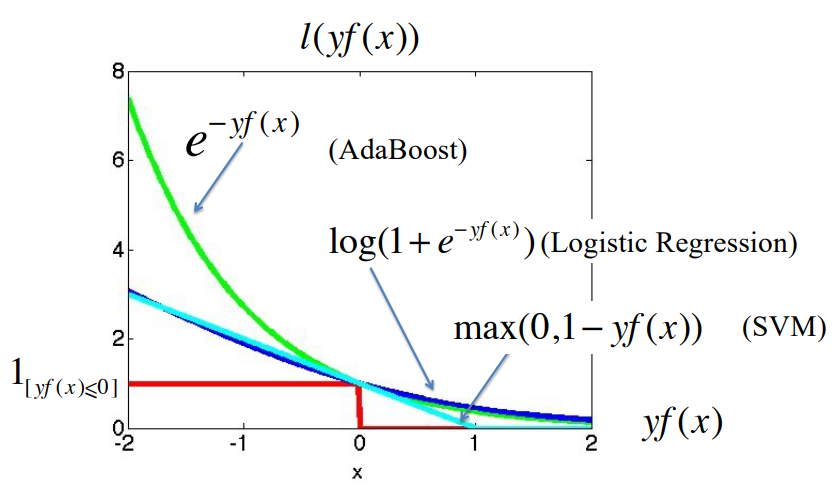
\includegraphics[scale=0.35]{loss_functions_class.png}
\end{center}

In the perceptron, we would want a function that penalizes not only if there is a misclassification, but how \textit{far} that misclassified point is from the boundary. Therefore, if $y^{(n)}$ and $h_\mathbf{w} (\mathbf{x}^{(n)})$ have the same sign, i.e. if $y^{(n)} h_\mathbf{w} (\boldsymbol{\phi}^{(n)}) > 0$, then the penalty should be $0$, and if it is $< 0$, then the penalty should be proportional to the orthogonal distance of the misclassified point to the boundary, which is represented by $-\mathbf{w}^T \boldsymbol{\phi}^{(n)} y^{(n)}$ (where the negative sign makes this cost term positive). To define our final cost function, let us define the function 
\[[f(\mathbf{x})]_+ \coloneqq \begin{cases} f(\mathbf{x}) & \text{ if } f(\mathbf{x}) > 0 \\ 0 & \text{ else } \end{cases}\]
Therefore, our cost functions would take all the points and penalize all the terms by $0$ if they are correctly classified and by $-\mathbf{w}^T \boldsymbol{\phi}^{(n)} y^{(n)}$ if incorrectly classified. 
\[E(\mathbf{w}) = \sum_{n=1} [ -\mathbf{w}^T \boldsymbol{\phi}^{(n)} y^{(n)} ]_+\]
which is a piecewise linear function and therefore can be optimized. In fact, it can be proven that if a dataset is \textbf{linearly separable}, i.e. if there exists an affine hyperplane separating the two classes, then the perceptron is guaranteed to find it. Therefore, the gradient descent algorithm
\[\mathbf{w}^{(\tau + 1)} = \mathbf{w}^{(\tau)} - \eta \nabla E(\mathbf{w})\]
which is easier to interpret as SGD updating one partial at a time
\[\mathbf{w}^{(\tau + 1)} = \mathbf{w}^{(\tau)} - \eta \frac{\partial E(\mathbf{w})}{\partial w_n} \bigg|_{\mathbf{w}^{(\tau)}}\]
where by abuse of notation, the partial represents the vector of $0$'s except for the $n$th term, will convergence to a solution if one exists. However, it does not guarantee that every step of GD will reduce the error. 

Let's implement this in scikit-learn, using two pipelines with different data standardization techniques to see the differences in the perceptron boundary. 
\begin{cverbatim}
from sklearn.pipeline import Pipeline 
from sklearn.linear_model import Perceptron
from sklearn.preprocessing import QuantileTransformer, StandardScaler

pipe1 = Pipeline([ 
    ("scale", StandardScaler()), 
    ("model", Perceptron())
])

pipe2 = Pipeline([
    ("scale", QuantileTransformer(n_quantiles=100)), 
    ("model", Perceptron())
])
\end{cverbatim}
which results in the following shown in Figure \ref{fig:Percepton_on_Standardized_data}. 
\begin{figure}[hbt!]
    \centering
    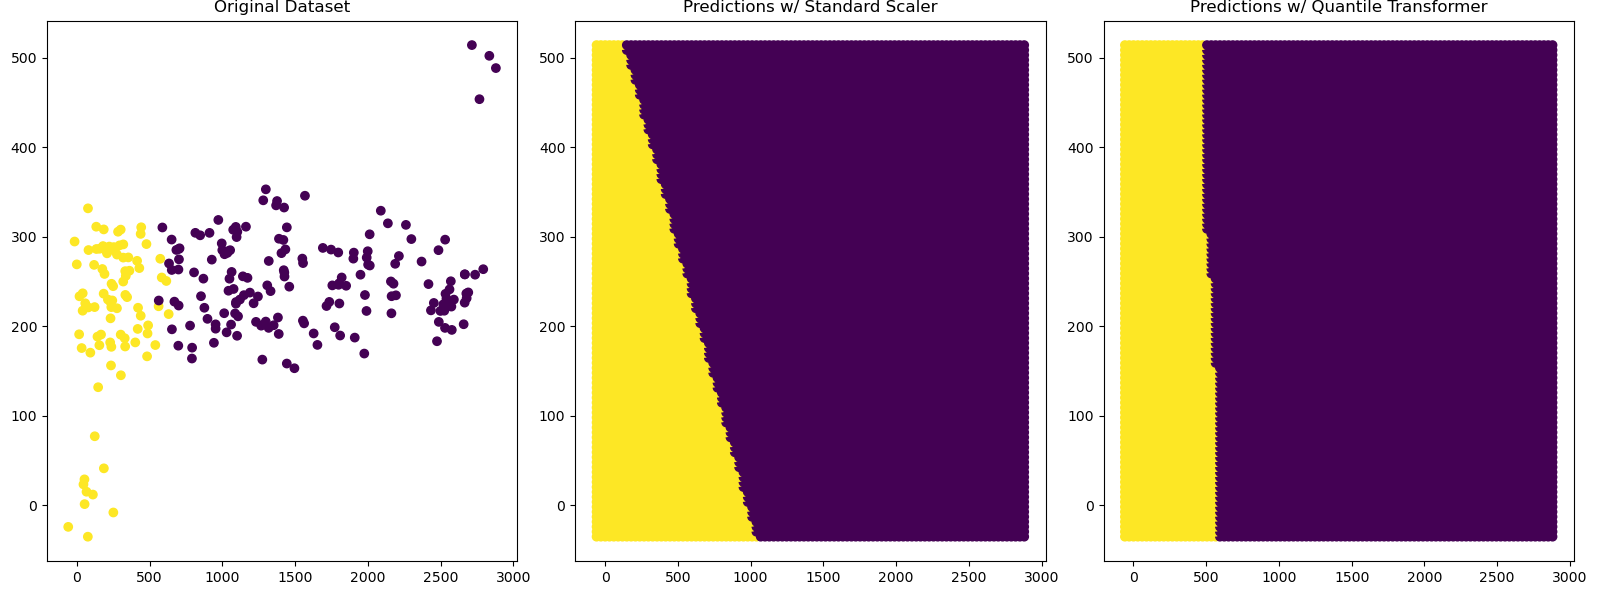
\includegraphics[scale=0.4]{Section_3/Perceptron.png}
    \caption{Perceptron Trained on Different Standardized Data}
    \label{fig:Percepton_on_Standardized_data}
\end{figure}


\section{Logistic Regression}

We can upgrade from a discriminant function to a discriminative probabilistic model with \textbf{logistic regression}. 

\begin{definition}[Logistic Regression]
The \textbf{logistic regression} model is a linear model of the form 
\[h_\theta (x) = \sigma (\theta^T x) = \frac{1}{1 + e^{- \theta^T x}}, \text{ where } \sigma(x) \coloneqq \frac{1}{1 + e^{x)}}\]
It is different from linear regression in two ways: 
\begin{enumerate}
    \item In linear regression, we assumed that the targets are linearly dependent with the covariates as $y = \mathbf{w}^T \mathbf{x} + b$. However, this means that the hypothesis $h_\mathbf{w}$ is unbounded. Since we have two classes (say with labels $0$ and $1$), we must have some sort of \textit{link function} $\sigma$ that takes the real numbers and compresses it into the domain $[0, 1]$. Technically, we can choose any continuous, monotinically increasing function from $\mathbb{R}$ to $(0, 1)$. However, the following property of the sigmoid makes derivation of gradients very nice. 
    \[\sigma^\prime (x) = \sigma(x) \, \big(1 - \sigma(x) \big)\]

    \item Once this is compressed, we assume that the residual distribution is a Bernoulli. 
\end{enumerate}
\end{definition}

One important observation to make is that notice that the output of our hypothesis is used as a parameter to define our residual distribution. 
\begin{enumerate}
    \item In linear regression, the $h_\mathbf{w}$ was used as the \textit{mean} $\mu$ of a Gaussian. 
    \item In logistic regression, the $h_\mathbf{w}$ is used also as the mean $p$ of a Bernoulli. 
\end{enumerate}
Some questions may arise, such as ``why isn't the variance parameter of the Gaussian considered in the linear model?" or ``what about other residual distributions that have multiple parameters?" This is all answered by generalized linear models, which uses the output of a linear model as a \textit{natural parameter} of the canonical exponential family of residual distributions. 

\subsection{Likelihood Estimation}

Unfortunately, there is no closed form solution for logistic regression like the least squares solution in linear regression. Therefore, we can only resort to maximum likelihood estimation. Given a dataset $\mathcal{D} = \{(x^{(i)}, y^{(i)})\}_{i=1}^N$, our likelihood is 
\[L(\theta ; \mathcal{D}) = \prod_{i=1}^n p(y^{(i)} \;|\; x^{(i)} ; \theta) = \prod_{i=1}^N  \big( h_\theta (x^{(i)} )\big)^{y^{(i)}} \; \big( 1 - h_\theta (x^{(i)})\big)^{1-y^{(i)}}\]
We can equivalently minimize its negative log likelihood, giving us the \textbf{binary cross entropy} loss function
\begin{align*}
    \ell(\theta) & = -\log L(\theta) \\
    & = -\sum_{i=1}^n y^{(i)} \log h_\theta (x^{(i)}) + (1 - y^{(i)}) \log (1 - h_\theta (x^{(i)}))
\end{align*}
Now taking the gradient for just a single sample $(x^{(i)}, y^{(i)})$ gives 
\begin{align*}
    \frac{\partial \ell}{\partial \theta}  & = \bigg( \frac{y^{(i)}}{\sigma(\theta^T x^{(i)})} - \frac{1 - y^{(i)}}{1 - \sigma(\theta^T x^{(i)})} \bigg) \, \frac{\partial}{\partial \theta} \sigma (\theta^T x^{(i)}) \\
    & = \frac{\sigma(\theta^T x^{(i)}) - y^{(i)}}{\sigma(\theta^T x^{(i)}) \, \big( 1 - \sigma(\theta^T x^{(i)}) \big)} \sigma(\theta^T x^{(i)}) \, \big( 1 - \sigma(\theta^T x^{(i)}) \big) x^{(i)} \\
    & = \big( h_\theta (x^{(i)}) - y^{(i)} \big) x
\end{align*}
and summing it over some minibatch $M \subset \mathcal{D}$ gives 
\[\nabla_\theta \ell_M = \sum_{(x, y) \in M} (y - h_\theta(x)) x\]
Therefore, the stochastic gradient descent algorithm is 
\begin{align*}
    \theta & = \theta - \eta \nabla_\theta \ell (\theta) \\
    & = \theta - \eta \sum_{(x, y) \in M} (y - h_\theta(x)) x
\end{align*}

\section{Softmax Regression}

The softmax function is defined 
\[o(\mathbf{x}) = \frac{e^{\mathbf{x}}}{||e^{\mathbf{x}}||} = \frac{1}{\sum_j e^{x_j}}\begin{pmatrix} e^{x_1} \\ \vdots \\ e^{x_D} \end{pmatrix}\]
The total derivative of the softmax can be derived as such. 

\begin{lemma}[Derivative of Softmax]
The derivative of the softmax is 
\[D o (\mathbf{x}) = \mathrm{diag}(o (\mathbf{x})) - o (\mathbf{x}) \otimes o (\mathbf{x})\]
where $\otimes$ is the outer product. That is, let $y_i$ be the output of the softmax. Then, for the $4 \times 4$ softmax function, we have 
\[D o(\mathbf{x}) = \begin{pmatrix} y_1 (1 - y_1) & - y_1 y_2 & -y_1 y_3 & - y_1 y_4 \\ -y_2 y_1 & y_2 (1 - y_2) & - y_2 y_3 & - y_2 y_4 \\ -y_3 y_1 & y_3 y_3 & y_3 (1 - y_3) & -y_3 y_4 \\ -y_4 y_1 & -y_4 y_2 & -y_4 y_3 & y_4 (1 - y_4) \end{pmatrix} \]
\end{lemma}
\begin{proof}
We will provide a way that allows us not to use quotient rule. Given that we are taking the partial derivative of $y_i$ with respect to $x_j$, we can use the log of it to get 
\[\frac{\partial}{\partial x_j} \log (y_i) = \frac{1}{y_i} \frac{\partial y_i}{\partial x_j} \implies \frac{\partial y_i}{\partial x_j} = y_i \, \frac{\partial}{\partial x_j} \log(y_i)\]
Now the partial of the log term is 
\begin{align*}
    \log{y_i} & = \log \bigg( \frac{e^{x_i}}{\sum_l e^{x_l}} = x_i - \log \bigg( \sum_l e^{x_l}\bigg) \\
    \frac{\partial}{\partial x_j} \log(y_i) & = \frac{\partial x_i}{\partial x_j} - \frac{\partial}{\partial x_j} \log \bigg( \sum_l e^{x_l}\bigg) \\
    & = 1_{i = j} - \frac{1}{\sum_l e^{x_l}} e^{x_j}
\end{align*}
and plugging this back in gives 
\[\frac{\partial y_i}{\partial x_j} = y_i (1_{i = j} - y_j)\]
\end{proof}

It also turns out that the sigmoid is a specific case of the softmax. That is, given softmax for 2 classes, we have 
\[o\begin{pmatrix} x_1 \\ x_2 \end{pmatrix} = \frac{1}{e^{x_1} + e^{x_2}} \begin{pmatrix} e^{x_1} \\ e^{x_2} \end{pmatrix}\]
So, the probability of being in class $1$ is 
\[\frac{e^{x_1}}{e^{x_1} + e^{x_2}} = \frac{1}{1 + e^{x_2 - x_1}}\]
and the logistic sigmoid is just a special case of the softmax function that avoids using redundant parameters. We actually end up overparameterizing the softmax because the probabilities must add up to one. 

\begin{definition}
The softmax regression of $K$ classes assumes a model of the form 
\[h_\theta (x) = o ( \mathbf{W} \mathbf{x} + \mathbf{b})\]
where $\mathbf{W} \in \mathbb{R}^{K \times D}, \mathbf{b} \in \mathbb{R}^D$. Again, we have a linear map followed by some link function (the softmax) which allows us to nonlinearly map our unbounded linear outputs to some domain that can be easily parameterized by a probability distribution. In this case, our residual distribution is a \textbf{multinomial distribution} 
\[y \sim \mathrm{Multinomial}\big( h_\mathbf{w} (\mathbf{x}) \big) = \mathrm{Multinomial}\big( [h_\mathbf{w} (\mathbf{x})]_1, \ldots, [h_\mathbf{w} (\mathbf{x})]_K \big) \]
\end{definition}

Notice again that the parameters of our residual distribution, the multinomial, is described with the output of our hypothesis function $h_{\boldsymbol{\theta}}$. 

\subsection{Likelihood Estimation}

Since a closed form solution is not available for logistic regression, it is clearly not available for softmax. Therefore, we one hot encode our target variables as $\mathbf{y}^{(i)}$ and write our likelihood as 
\[L(\theta; \mathcal{D}) = \prod_{i=1}^N \prod_{k=1}^K p(C_k \mid \mathbf{x}^{(i)})^{\mathbf{y}^{(i)}_k} = \prod_{i=1}^N \prod_{k=1}^K \big( \mathbf{h}_\mathbf{W} (\mathbf{x}^{(i)})\big)_k^{\mathbf{y}_k^{(i)}} \]
Taking the negative logarithm gives us the \textbf{cross entropy} loss function
\[\ell (\boldsymbol{\theta}) = - \sum_{i=1}^N \sum_{k=1}^K y^{(i)}_k \log \big( \mathbf{h}_{\boldsymbol{\theta}} (\mathbf{x}^{(i)})\big)_k = - \sum_{i=1}^N \mathbf{y}^{(i)} \dot \log \big( \mathbf{h}_{\boldsymbol{\theta}} (\mathbf{x}^{(i)} \big) \]
where $\cdot$ is the dot product. The gradient of this function may seem daunting, but it turns out to be very cute. Let us take a single sample $(\mathbf{x}^{(i)}, \mathbf{y}^{(i)})$, drop the index $i$, and write
\begin{align*}
    \mathbf{x} & \mapsto \mathbf{W} \mathbf{x} + \mathbf{b} = \mathbf{z} \\
    \hat{\mathbf{y}} = \mathbf{a} & = o (\mathbf{z}) \\
    L & = - \mathbf{y} \cdot \log (\mathbf{a}) = - \sum_{k=1}^K y_k \log(a_k)
\end{align*}
We must compute 
\[\frac{\partial L}{\partial \mathbf{W}} = \frac{\partial L}{\partial \mathbf{a}} \frac{\partial \mathbf{a}}{\partial \mathbf{z}} \frac{\partial \mathbf{z}}{\partial \boldsymbol{\theta}}\]
We can compute $\partial L /\partial \mathbf{z}$ as such, using our derivations for the softmax derivative above. We compute element wise. 
\begin{align*}
    \frac{\partial L}{\partial z_j} & = - \sum_{k=1}^K y_k \, \frac{\partial}{\partial z_j} \log (a_k) \\
    & = - \sum_{k=1}^K y_k \frac{1}{a_k} \frac{\partial a_k}{\partial z_j} \\
    & = - \sum_{k=1}^K \frac{y_k}{a_k} \, a_k (1_{\{k = j\}} - a_j) \\
    & = - \sum_{k=1}^K y_k (1_{\{k = j\}} - a_j) \\
    & = \bigg( \sum_{k=1}^K y_k a_j \bigg) - y_j \\
    & = a_j \bigg( \sum_{k=1}^K y_k \bigg) - y_j \\
    & = a_j - y_j
\end{align*}
and combining these gives 
\[\frac{\partial L}{\partial \mathbf{z}} = (\mathbf{a} - \mathbf{y})^T\]
Now, computing $\partial \mathbf{z} / \partial \mathbf{W}$ gives us a $3$-tensor, which is not ideal to work with. However, let us just compute this with respect to the elements again. We have 
\begin{align*}
    z_k & = \sum_{d=1}^D W_{kd} x_d + b_k \\ 
    \frac{\partial z_k}{\partial W_{ij}} & = \sum_{d=1}^D x_d \frac{\partial}{\partial W_{ij}} W_{kd}
\end{align*}
where 
\[\frac{\partial}{\partial W_{ij}} W_{kd} = \begin{cases} 1 & \text{ if } i = k, j = d \\ 0 & \text{ else} \end{cases}\]
Therefore, since $d$ is iterating through all elements, the sum will only be nonzero if $k = i$. That is, $\frac{\partial z_k}{\partial W_{ij}} = x_j$ if $k = i$ and $0$ if else. Therefore, 
\begin{center}
    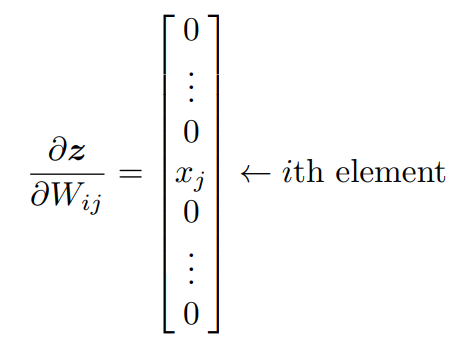
\includegraphics[scale=0.3]{softmax_deriv.png}
\end{center}
Now computing 
\[\frac{\partial L}{\partial W_{ij}} = \frac{\partial L}{\partial \mathbf{z}} \frac{\partial \mathbf{z}}{\partial W_{ij}} = (\mathbf{a} - \mathbf{y}) \frac{\partial \mathbf{z}}{\partial W_{ij}} = \sum_{k=1}^K (a_k - y_k) \frac{\partial z_k}{\partial W_{ij}} = (a_i - y_i) x_j\]
To get $\partial L / \partial W_{ij}$ we want a matrix whose entry $(i, j)$ is $(a_i - y_i) x_j$. This is simply the outer product as shown below. For the bias term, $\partial \mathbf{z} / \partial \mathbf{b}$ is simply the identity matrix. 
\[\frac{\partial L}{\partial \mathbf{W}} = (\mathbf{a} - \mathbf{y}) \mathbf{x}^T, \;\;\;\; \frac{\partial L}{\partial \mathbf{b}} = \mathbf{a} - \mathbf{y}\]


Therefore, summing the gradient over some minibatch $M \subset [N]$ gives 
\[\nabla_{\mathbf{W}} \ell_M = \sum_{i \in M} (\mathbf{h}_{\boldsymbol{\theta}}(\mathbf{x}^{(i)}) - \mathbf{y}^{(i)}) (\mathbf{x}^{(i)})^T, \;\;\;\;\; \nabla_{\mathbf{b}} \ell_M = \sum_{i \in M} (\mathbf{h}_{\boldsymbol{\theta}}(\mathbf{x}^{(i)}) - \mathbf{y}^{(i)})\]
and our stochastic gradient descent algorithm is 
\begin{align*}
    \boldsymbol{\theta} = \begin{pmatrix} \mathbf{W} \\ \mathbf{b} \end{pmatrix} & = \begin{pmatrix} \mathbf{W} \\ \mathbf{b} \end{pmatrix} - \eta \begin{pmatrix} \nabla_{\mathbf{W}} \ell_M \\ \nabla_{\mathbf{b}} \ell_M \end{pmatrix} \\
    & = \begin{pmatrix} \mathbf{W} \\ \mathbf{b} \end{pmatrix} - \eta \begin{pmatrix} \sum_{i \in M} (\mathbf{h}_{\boldsymbol{\theta}}(\mathbf{x}^{(i)}) - \mathbf{y}^{(i)}) (\mathbf{x}^{(i)})^T \\ \sum_{i \in M} (\mathbf{h}_{\boldsymbol{\theta}}(\mathbf{x}^{(i)}) - \mathbf{y}^{(i)}) \end{pmatrix} 
\end{align*}

\section{Generalized Linear Models}

Remember the linear model looked like this, where we use the conventional $\beta$ notation to represent parameters. 
\[Y = X^T \beta + \epsilon, \;\; \epsilon \sim N(0, \sigma^2 I)\]
which implies that $Y \mid X \sim N(X^T \beta, \sigma^2 I)$. Basically, given $x$, I assume some distribution of $Y$, and the value of $x$ will help me guess what the mean of this distribution is. Note that we in here assume that only the mean depends on $X$. I could potentially have something crazy, like 
\[Y \mid X \sim N(X^T \beta, (X^T \gamma) (X X^T + I))\]
where the covariance will depend on $X$, too, but in this case we only assume that that mean is dependent on $X$. 
\[Y \mid X \sim N(\mu(X), \sigma^2 I)\]
where in the linear model, $\mu(X) = X^T \beta$. So, there are three assumptions we are making here: 
\begin{enumerate}
    \item $Y \mid X$ is Gaussian. 
    \item $X$ only affects the mean of $Y \mid X$, written $\mathbb{E}[Y \mid X] = \mu(X)$. 
    \item $X$ affects the mean in a linear way, such that $\mu(X) = X^T \beta$. 
\end{enumerate}
So the two things we are trying to relax are: 
\begin{enumerate}
    \item \textbf{Random Component}: the response variable $Y \mid X$ is continuous and normally distributed with mean $\mu = \mu(X) = \mathbb{E}[Y \mid X]$. 
    \item \textbf{Link}: I have a link that explains the relationship between the $X$ and the $\mu$, and this relationship is $\mu(X) = X^T \beta$. 
\end{enumerate}
So when talking about GLMs, we are not changing the fact that we have a linear function $X \mapsto X^T \beta$. However, we are going to assume that $Y \mid X$ now comes from a broader \textbf{family of exponential distributions}. Second, we are going to assume that there exists some \textbf{link function} $g$
\[g(\mu(X)) = X^T \beta\]
Admittedly, this is not the most intuitive way to think about it, since we would like to have $\mu(X) = f(X^T \beta)$, but here we just decide to call $f = g^{-1}$. Therefore, if I want to give you a GLM, I just need to give you two things: the conditional distribution $Y \mid X$, which can be any distribution in the exponential family, and the link function $g$. 

We really only need this link function due to compatibility reasons. Say that $Y \mid X \sim \mathrm{Bern}(p)$. Then, $\mu(X) = \mathbb{E}[Y \mid X]$ always lives in $[0, 1]$, but $X^T \beta$ always lives in $\mathbb{R}$. We want our model to be realistic, and we can clearly see the problem shown in Figure \ref{fig:Bernoulli_GLM}. 
\begin{figure}
    \centering
    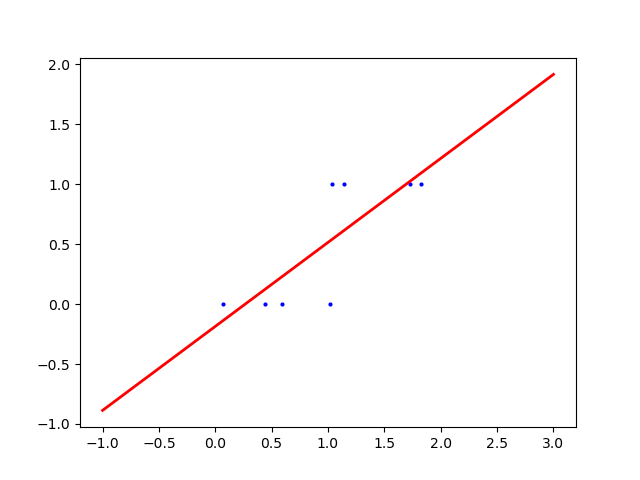
\includegraphics[scale=0.5]{Section_4/GLM_bernoulli.png}
    \caption{Fitting a linear model for Bernoulli random variables will predict a mean that is outside of $[0, 1]$ when getting new datapoints. }
    \label{fig:Bernoulli_GLM}
\end{figure}
If $Y \mid X$ is some exponential distribution, then its support is always positive and so $\mu(X) > 0$. But if we stick to the old form of $\mu(X) = X^T \beta$, then $\mathrm{Im}(\mu) = \mathbb{R}$, which is not realistic when we predict negative values. Let's take a couple examples: 

\begin{example}
In the early stages of a disease epidemic, the rate at which new cases occur can often increase exponentially through time. Clearly, $\mu(X) = \mathbb{E}[Y \mid X]$ should be positive and we should have some sort of exponential trend. Hence, if $\mu(x)$ is the expected number of cases on data $x$, a model of the form 
\[\mu(x) = \gamma \exp (\delta x)\]
seems appropriate, where $\gamma$ and $\delta$ are simply scaling factors. Clearly, $\mu(X)$ is not of the form $f(X^T \beta)$. So what I do is to transform $\mu$ in such a way that I can get something that is linear. 
\[\log(\mu(X)) = \log(\gamma) + \delta X\]
which is now linear in $X$, of form $\beta_0 + \beta_1 X$. This will have some effects, but this is what needs to be done to have a genearlized linear model. Note that what I did to $\mu$ was take the log of it, and so the link function is $g = \log$, called the \textbf{log-link}. Now that we have chosen the $g$, we still need to choose what the conditional distribution $Y \mid X$ would be. This is determined by speaking with industry professionals, experience, and convenience. In this case, $Y$ is a count, and since this must be a discrete distribution. Since it is not bounded above, we think Poisson. 
\end{example}

\begin{example}
The rate of capture of preys, $Y$, by a hunting animal, tends to increase with increasing density of prey $X$, but eventually level off when the predator is catching as much as it can cope with. We want to find a perhaps concave function that levels off, and suitable model might be 
\[\mu(X) = \frac{\alpha X}{h + X}\]
where $\alpha$ represents the maximum capture rate, and $h$ represents the prey density at which the capture rate is half the maximum rate. Again, we must find some transformation $g$ that turns this into a linear function of $X$, and what we can do it use the \textbf{reciprocal-link}. 
\[\frac{1}{\mu(X)} = \frac{h + X}{\alpha X} = \frac{h}{\alpha} \frac{1}{X} + \frac{1}{\alpha}\]
The standard deviation of capture rate might be approximately proportional to the mean rate, suggesting the use of a Gamma distribution for the response. 
\end{example}

\begin{example}
The Kyphosis data consist of measurements on $81$ children following corrective spinal surgery. The binary response variable, Kyphosis, indicates the presence or absence of a postoperative deforming. The three covariates are: age of the child in months, number of the vertebrae involved in the operation, and the start of the range of the vertebrae involved. The response variable is binary so there is no choice: $Y \mid X$ is Bernoulli with expected value $\mu(X) \in (0, 1)$. We cannot write $\mu(X) = X^T \beta$ because the right hand side ranges through $\mathbb{R}$, and so we find an invertible function that squishes $\mathbb{R}$ to $(0, 1)$, and so we can choose basically any CDF. 
\end{example}

For clarification, when writing a distribution like $\mathrm{Bernoulli}(p)$, or $\mathrm{Binomial}(n, p)$, $\mathrm{Poisson}(\lambda)$, or $N(\mu, \sigma^2)$, the hyperparameters that we usually work with we will denote as $\boldsymbol{\theta}$, and the space that this $\boldsymbol{\theta}$ lives in will denote $\Theta$. For example, for the Bernoulli, $\Theta = [0, 1]$, and for Poisson, $\Theta = [0, +\infty)$. 

Ultimately, a GLM consists of three steps: 
\begin{enumerate}
    \item The observed input $X$ enters the model through a linear function $\beta^T X$. 
    \item The conditional mean of response, is represented as a function of the linear combination 
    \[\mathbb{E}[Y \mid X] = \mu = f(\beta^T X)\]
    \item The observed response is drawn from an exponential family distribution with conditional mean $\mu$. 
\end{enumerate}

\subsection{Exponential Family}

We can write the pdf of a distribution as a function of the input $x$ and the hyperparameters $\theta$, so we can write $P_\theta (x) = p(\theta, x)$. For now, let's think that both $x, \theta \in \mathbb{R}$. Think of all the functions that depend on $\theta$ and $x$. There are many of them, but we want $\theta$ and $x$ to interact in a certain way. The way that I want them to interact with each other is that they are multiplied within an exponential term. Now clearly, this is not a very rich family, so we are just slapping some terms that depend only on $\theta$ and only on $x$. 
\[p_\theta (x) = \exp(\theta x) h(x) c(\theta)\]
But now if $\theta \in \mathbb{R}^k$ and $x \in \mathbb{R}^q$, then we cannot simply take the product nor the inner product, but what we can do is map both of them into a space that has the same dimensions, so I can take the inner product. That is, let us map $\boldsymbol{\theta} \mapsto \boldsymbol{\eta}(\boldsymbol{\theta}) \in \mathbb{R}^k$ and $\mathbf{x} \mapsto \mathbf{T}(\mathbf{x}) \in \mathbb{R}^k$, and so 
our exponential distribution form would be generalized into something like 
\[p_{\boldsymbol{\theta}} (\mathbf{x}) = \exp\big[ \boldsymbol{\eta}(\boldsymbol{\theta}) \cdot \mathbf{T}(\mathbf{x}) \big] h(\mathbf{x}) c(\boldsymbol{\theta})\]
We can think of $c(\boldsymbol{\theta})$ as the normalizing term that allows us to integrate the pdf to $1$. 
\[\int_\mathcal{X} p_{\boldsymbol{\theta}} (\mathbf{x}) = c(\boldsymbol{\theta}) \int \exp\big[\boldsymbol{\eta}(\boldsymbol{\theta}) \cdot \mathbf{T}(\mathbf{x}) \big] h(\mathbf{x})  \,d\mathbf{x}\]
We can just push the $c(\boldsymbol{\theta})$ term into the exponential by letting $c(\boldsymbol{\theta}) = e^{-\log(c(\boldsymbol{\theta}))^{-1}}$ to get our definition. 


\begin{definition}[Exponential Family]
A \textbf{k-parameter exponential family} is a family of distributions with pdf/pmf of the form 
\[p_{\boldsymbol{\theta}} (\mathbf{x}) = \exp\big[ \boldsymbol{\eta}(\boldsymbol{\theta}) \cdot \mathbf{T}(\mathbf{x}) - B(\boldsymbol{\theta}) \big] h(\mathbf{x})\]
The $h$ term, as we will see, will not matter in our maximum likelihood estimation, so we keep it outside the exponential. 
\begin{enumerate}
    \item $\boldsymbol{\eta}$ is called the \textbf{canonical parameter}. Given a distribution parameterized by the regular hyperparameters $\boldsymbol{\theta}$, we would like to parameterize it in a different way $\boldsymbol{\eta}$ under the function $\boldsymbol{\eta}: \Theta \rightarrow \mathbb{R}$

    \item $\mathbf{T}(\mathbf{x})$ is called the \textbf{sufficient statistic}. 

    \item $h(\mathbf{x})$ is a nonnegative scalar function. 

    \item $B(\boldsymbol{\theta})$ is the normalizing factor. 
\end{enumerate}
\end{definition}

Let's look at some examples. 

\begin{example}[Gaussian]
If we put the coefficient into the exponential and expand the square term, we get 
\[p_\theta (x) = \exp \bigg( \frac{\mu}{\sigma^2} \cdot x - \frac{1}{2\sigma^2} \cdot x^2 - \frac{\mu^2}{2 \sigma^2} - \log ( \sigma \sqrt{2 \pi}) \bigg)\] 
where 
\[\boldsymbol{\eta}(\boldsymbol{\theta}) = \begin{pmatrix} \mu /\sigma^2 \\ -1 / 2 \sigma^2 \end{pmatrix}, \; T(x) = \begin{pmatrix} x \\ x^2 \end{pmatrix}, \; B(\theta) = \frac{\mu^2}{2 \sigma^2} + \log(\sigma \sqrt{2 \pi}), \; h(x) = 1\]
This is not a unique representation since we can take the $\log(\sqrt{2 \pi})$ out of the exponential, but why bother to do this when we can just stuff everything into $B$ and keep $h$ simple. 
\end{example}

\begin{example}[Gaussian with Known Variance]
If we have known variance, we can write the Gaussian pdf as 
\[p_\theta (x) = \exp \bigg[ \frac{\mu}{\sigma} \cdot \frac{x}{\sigma} - \frac{\mu^2}{2 \sigma^2} \bigg] \cdot \frac{1}{\sigma \sqrt{2\pi}} e^{x^2/2 \sigma^2}\]
where 
\[\eta(\theta) = \frac{\mu}{\sigma}, \; T(x) = \frac{x}{\sigma}, \; B(\theta) = \frac{\mu^2}{2 \sigma^2}, \; h(x) = \frac{1}{\sigma \sqrt{2 \pi}} e^{x^2/2 \sigma^2}\]
\end{example}

\begin{example}[Bernoulli]
The pmf of a Bernoulli with $\theta$ is 
\begin{align*}
    p_\theta (x) & = \theta^x (1 - \theta)^{(1 - x)} \\
    & = \exp \big[x \log (\theta) + (1 - x)\log(1 - \theta) \big] \\
    & = \exp \bigg( x \log \Big[ \frac{\theta}{1 - \theta} \Big] - \log \Big[ \frac{1}{1 - \theta} \Big] \bigg)
\end{align*}
where 
\[\eta(\theta) = \log \Big[ \frac{\theta}{1 - \theta} \Big], \; T(x) = x, \; B(\theta) = \log \Big[ \frac{1}{1 - \theta} \Big], \; h(x) = 1\]
\end{example}


\begin{example}[Binomial with Known Number of Trials]
We can transform a binomial with known $N$ as 
\begin{align*}
    p_\theta (x) &  = {N \choose x} \theta^x  (1 - \theta)^{1 - x} \\
    & = \exp \bigg[ x \ln \big( \frac{\theta}{1 - \theta} \Big) + \ln(1 - \theta) \bigg] \cdot {N \choose x} 
\end{align*}
where 
\[\eta (\theta) = \ln \big( \frac{\theta}{1 - \theta} \Big), \; T(x) = x, \; B(\theta) = \ln(1 - \theta), \; h(x) = {N \choose x}\]
\end{example}

\begin{example}[Poisson]
The pmf of Poisson with $\theta$ can be expanded 
\begin{align*}
    p_\theta & = \frac{\theta^{-x}}{x!} e^{-\theta} \\
    & = \exp \big[ -\theta + x\log(\theta) - \log(x!) \big] \\
    & = \exp \big[ x \log(\theta) - \theta \big] \, \frac{1}{x!}
\end{align*}
where 
\[\eta(\theta) = \log(\theta), \; T(x) = x, \; B(\theta) = \theta, \; h(x) = \frac{1}{x!}\]
\end{example}

However, the uniform is not in here. In fact, any distribution that has a support that does not depend on the parameter is not an exponential distribution. 

Let us now focus on one parameter families where $\theta \in \Theta \subset \mathbb{R}$, which do not include the Gaussian (with unknown mean and variance, Gamma, multinomial, etc.), which has a pdf written in the form 
\[p_\theta (x) = \exp \big[ \eta (\theta) \, T(x) - B(\theta) \big] \, h(x)\]


\subsubsection{Canonical Exponential Family}

Now a common strategy in statistical analysis is to reparamaterize a probability distribution. Suppose a family of probability distributions $\{P_\theta\}$ is parameterized by $\theta \in \Theta \subset \mathbb{R}$. If we have an invertible function $\eta: \Theta \rightarrow \mathcal{T} \subset \mathbb{R}$, then we can paramaterize the same family with $\eta$ rather than $\theta$, with no loss of information. Typically, it is the case that $\eta$ is invertible for exponential families, so we can just reparameterize the whole pdf and write 
\[p_\eta (x) = \exp \big[ \eta \, T(x) - \phi(\eta) \big] \, h(x)\]
where $\phi = B \circ \eta^{-1}$. 

\begin{definition}[Canonical One-Parameter Exponential Family]
A family of distributions is said to be in \textbf{canonical one-parameter exponential family} if its density is of form 
\[p_\eta (x) = \exp \big[ \eta \, T(x) - \phi(\eta) \big] \, h(x)\]
which is a subfamily of the exponential family. The function $\psi$ is called the \textbf{cumulant generating function}. 
\end{definition}

Before we move on, let us just provide a few examples. 

\begin{example}[Poisson]
The Poisson can be represented as 
\[p_\theta (x) = \exp \big[ x \log{\theta} - \theta \big] \, \frac{1}{x!}\]
Now let $\eta = \log{\theta} \implies \theta = e^{\eta}$. So, we can reparamaterize the density as 
\[p_\eta(x) = \exp \big[ x \eta - e^\eta \big] \, \frac{1}{x!}\]
where $P_\eta = \mathrm{Poisson}(e^\eta)$ for $\eta \in \mathcal{T} = \mathbb{R}$, compared to $P_\theta = \mathrm{Poisson}(\theta)$ for $\theta \in \Theta = \mathbb{R}^+$. 
\end{example}

\begin{example}[Gaussian]
Recall that the Gaussian with known parameter $\sigma^2$ and unknown $\theta = \mu$ is in the exponential family, since we can expand it as 
\[p_\theta (x) = \exp \bigg[ \frac{\mu}{\sigma^2} \cdot x - \frac{\mu^2}{2 \sigma^2} \bigg] \cdot \frac{1}{\sigma \sqrt{2\pi}} e^{x^2/2 \sigma^2}\]
We can perform the change of parameter $\eta = \mu^2 / 2\sigma^2 \implies \mu = \sigma^2 \eta$, and substituting this in will give the canonical representation 
\[p_\eta (x) = \exp \Big[ \eta x - \frac{\sigma^2 \eta^2}{2} \Big] \cdot \frac{1}{\sigma \sqrt{2\pi}} e^{x^2/2 \sigma^2}\]
where now $P_\eta = N(\sigma^2 \eta, \sigma^2)$ for $\eta \in \mathcal{T} = \mathbb{R}$, compared to $P_\theta = N(\theta, \sigma^2)$ for $\theta \in \Theta = \mathbb{R}$, which is basically the same space. 
\end{example}

\begin{example}[Bernoulli]
The Bernoulli has an exponential form of 
\[p_\theta (x) = \exp \bigg[ x \log \Big( \frac{\theta}{1 - \theta} \Big) + \log(1 - \theta)\bigg]\]
Now setting $\eta = \log\big( \frac{\theta}{1 - \theta} \big) \implies \theta = \frac{1}{1 + e^{-\eta}}$, and so $B(\theta) = - \log(1 - \theta) = - \log \big( \frac{e^{-\eta}}{1 + e^{-\eta}} \big) = \log(1 + e^\eta) = \psi(\eta)$, and so the canonical paramaterization is 
\[p_\eta (x) = \exp \big[ x \eta - \log(1 + e^{\eta}) \big]\]
\end{example}


We present two useful properties of the exponential family. 

\begin{theorem}[Moments]
Let random variable $X$ be in the canonical exponential family $P_\eta$ 
\[p_\eta (x) = e^{\eta T(x) - \psi(\eta)} h(x)\]
Then, the expectation and variance are encoded in the cumulant generating function in the following way 
\[\mathbb{E} [T(X)] = \psi^\prime (\eta) \;\;\;\;\;\;\;\; \Var[T(X)] = \psi^{\prime\prime} (\eta)\]
\end{theorem}
\begin{proof}

\end{proof}

\begin{example}
We show that this is consistent with the Poisson, normal, and Bernoulli distributions. 
\begin{enumerate}
    \item In the Poisson, $\psi(\eta) = e^{\eta}$, and so $\psi^\prime(\eta) = e^\eta = \theta = \mathbb{E}[X]$. Taking the second derivative gives $\psi^{\prime\prime}(\eta) = e^\eta = \theta = \Var[X]$, too. \
    
    \item In the Normal with known variance $\sigma^2$, we have $\psi(\eta) = \frac{1}{2} \sigma^2 \eta^2$. So 
    \begin{align*}
        \mathbb{E}[X] & = \psi^\prime (\eta) = \sigma^2 \eta = \mu \\
        \Var[X] & = \psi^{\prime\prime} (\eta) = \sigma^2
    \end{align*}

    \item In the Bernoulli, we have $\psi(\eta) = \log(1 + e^{-\eta})$. Therefore, 
    \begin{align*}
        \mathbb{E}[X] & = \psi^\prime (\eta) = \frac{x^\eta}{1 + x^{\eta}} = \frac{1}{1 + e^{-\eta}} = \theta \\
        \Var[X] & = \psi^{\prime\prime} (\eta) = -\bigg(\frac{1}{1 + e^{-\eta}}\bigg)^2 \, e^{-\eta} \cdot -1 = \theta^2 \cdot \frac{1 - \theta}{\theta} = \theta (1 - \theta) 
    \end{align*}
\end{enumerate}
\end{example}

\begin{theorem}[Convexity]
Consider a canonical exponential family with density 
\[p_\eta (x) = e^{\eta T(x) - \psi(\eta)} h(x)\]
and natural parameter space $\mathcal{T}$. Then, the set $\mathcal{T}$ is convex, and the cumulant generating function $\psi$ is convex on $\mathcal{T}$. 
\end{theorem}
\begin{proof}
This can be proven using Holder's inequality. However, from the theorem above, note that $\Var[T(X)] = \psi^{\prime\prime}(\eta)$ must be positive since we are talking about variance. This implies that the second derivative of $\psi$ is positive, and therefore must be convex. 
\end{proof}


% We will look at a subfamily of the exponential family. Now remember that we introduce the functions $\boldsymbol{\eta}$ and $\mathbf{T}$ so that we can capture a much broader range of distributions, but if we have one parameter $k = 1$, then we can just set $\boldsymbol{\eta}(\boldsymbol{\theta})$ to be the new parameter $\theta$. The \textbf{canonical exponential family} for $k = 1, y \in \mathbb{R}$, is defined to have the pdf 
% \[f_\theta (y) = \exp \bigg( \frac{y \theta - b(\theta)}{\phi} + c(y, \phi) \bigg)\]
% where 
% \[h(y) = \exp \big( c(y, \phi)\big) \]
% If $\phi$ is known, this is a one-parameter exponential family with $\theta$ being the \textbf{canonical parameter}, and if $\phi$ is unknown, the $h(y)$ term will not depend on $\theta$, which we may not be able to split up into the exponential pdf form. In this case $\phi$ is called the \textbf{dispersion parameter}. For now, we will always assume that $\phi$ is known. 

% We can prove this for all other classes, too. We can think of the $c(y, \phi)$ as just a term that we stuff every other term into. What really differentiates the different distributions of the canonical exponential family is the $b(\theta)$. The form of $b$ will determine whether this distribution is a Gaussian, or a Bernoulli, or etc. This $b$ will capture information about the mean, the variance, the likelihood, about everything. 

% \subsection{Cumulant Generating Function}

% \begin{definition}[Score]
% The \textbf{score} is the gradient of the log-likelihood function with respect to the parameter vector. That is, given that $L(\boldsymbol{\theta})$ is the likelihood, then 
% \[s(\boldsymbol{\theta}) \coloneqq \frac{\partial \log L(\boldsymbol{\theta}; \mathbf{x})}{\partial \boldsymbol{\theta}}\]
% which gives a row covector. 
% \end{definition}

% Now, remember that the score also depends on the observations $\mathbf{x}$. If we rewrite the likelihood as a probability density function $L(\boldsymbol{\theta}; \mathbf{x}) = f(\mathbf{x}; \boldsymbol{\theta})$, then we can say that the expected value of the score is equal to $0$, since 
% \begin{align*}
%     \mathbb{E}[s(\boldsymbol{\theta})] & = \int_\mathcal{X} f(\mathbf{x}; \boldsymbol{\theta}) \frac{\partial}{\partial \boldsymbol{\theta}} \log L (\boldsymbol{\theta}; \mathbf{x}) \,d\mathbf{x} \\
%     & = \int_\mathcal{X} f(\mathbf{x}; \boldsymbol{\theta}) \frac{1}{f(\mathbf{x}; \boldsymbol{\theta})} \, \frac{\partial f(\mathbf{x}; \boldsymbol{\theta})}{\partial \boldsymbol{\theta}} \,dx \\
%     & = \frac{\partial}{\partial \boldsymbol{\theta}} \int_\mathcal{X} f(\mathbf{x}; \boldsymbol{\theta}) \,d \mathbf{x} \\
%     & = \frac{\partial}{\partial \boldsymbol{\theta}} 1 = 0
% \end{align*}
% where we take a leap of faith in switching the derivative and integral in the penultimate line. Furthermore, we can get the second identity 
% \[\mathbb{E}\bigg[ \frac{\partial^2 \ell}{\partial \theta^2} \bigg] + \mathbb{E} \bigg[ \frac{\partial \ell}{\partial \theta} \bigg]^2 = 0\]

% We can apply these two identities as follows. Since 
% \[\ell (\theta) = \frac{Y \theta - b(\theta)}{\phi} + c(Y ; \phi)\]
% therefore 
% \[\frac{\partial \ell}{\partial \theta} = \frac{Y - b^\prime(\theta)}{\phi}\]
% which yields 
% \[0 = \mathbb{E} \bigg[ \frac{\partial \ell}{\partial \theta} \bigg] = \frac{\mathbb{E}[Y] - b^\prime(\theta)}{\phi} \implies \mathbb{E}[Y] = \mu = b^\prime(\theta)\]
% On the other hand, we have 
% \[\frac{\partial^2 \ell}{\partial \theta^2} + \bigg( \frac{\partial \ell}{\partial \theta} \bigg)^2 = -\frac{b^{\prime\prime} (\theta)}{\phi} + \bigg(\frac{Y - b^\prime (\theta)}{\phi} \bigg)^2\]
% and from the previous result, we get 
% \[\frac{Y - b^\prime(\theta)}{\phi} = \frac{Y - \mathbb{E}[Y]}{\phi}\]
% together with the second identity, yields 
% \[0 = -\frac{b^{\prime\prime}(\theta)}{\phi} + \frac{\Var(Y)}{\phi^2} \implies \Var(Y) = \phi \, ^{\prime\prime} (\theta)\]
% Since variance is always positive, this implies that $b^{\prime\prime} > 0$ and therefore $b$ must be convex. 

\subsection{Link Functions}

Now let's go back to GLMs. In linear models, we said that the conditional expectation of $Y$ given $X = \mathbf{x}$ must be a linear function in $x$ 
\[\mathbb{E}[Y \mid X = \mathbf{x}] = \mu(\mathbf{x}) = \mathbf{x}^T \beta\]
But if the conditional distribution takes values in some subset of $\mathbb{R}$, such as $(0, 1)$, then it may not make sense to write this as a linear function, since $X^T \beta$ has an image spanning $\mathbb{R}$. So what we need is a link function that relates, i.e. transforms the restricted subset of $\mu$, onto the real line, so that now you can express it of the form $X^T \beta$. 
\[g \big( \mu(X) \big) = X^T \beta\]
Again, it is a bit more intuitive to talk about $g^{-1}$, which takes our $X^T \beta$ and transforms it to the values that I want, so we will talk about both of them simultaneously. If $g$ is our link function, we want it to satisfy 3 requirements: 
\begin{enumerate}
    \item $g$ is continuously differentiable 
    \item $g$ is strictly increasing 
    \item $\mathrm{Im}(g) = \mathbb{R}$, i.e. it spans the entire real line
\end{enumerate}
This implies that $g^{-1}$ exists, which is also continuously differentable and is strictly increasing. 

\begin{example}
If I have a conditional distribution... 
\begin{enumerate}
    \item that is Poisson, then we want our $\mu$ to be positive, and so we need a link function $g: \mathbb{R}^+ \rightarrow \mathbb{R}$. One choice would be the logarithm 
    \[g(\mu(X)) = \log \big( \mu(X) \big) = X^T \beta\]

    \item that is Bernoulli, then we want our $\mu$ to be in $(0, 1)$ and we need a link function $g: (0, 1) \rightarrow \mathbb{R}$. There are 2 natural choices, which may be the \textbf{logit} function 
    \[g(\mu(X)) = \log \bigg( \frac{\mu(X)}{1 - \mu(X)} \bigg) = X^T \beta\]
    or the \textbf{probit} function 
    \[g(\mu(X)) = \Phi^{-1} \big(\mu(X)\big) = X^T \beta \]
    where $\Phi$ is the CDF of a standard Gaussian. The two functions can be seen in Figure \ref{fig:logit_probit}. 
    \begin{figure}
        \centering
        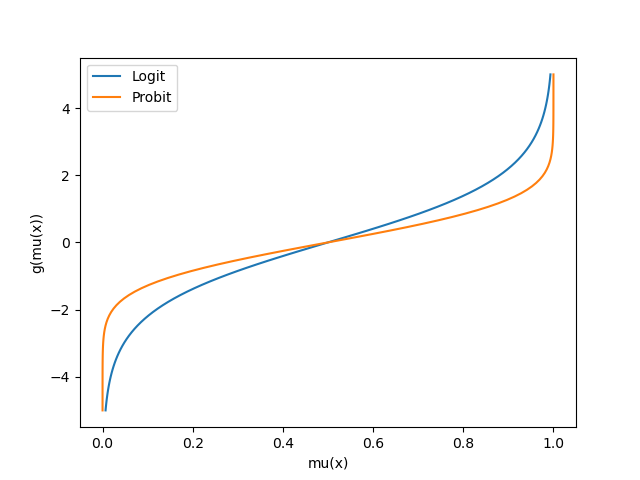
\includegraphics[scale=0.5]{Section_4/probit_logit.png}
        \caption{Logit and Probit Functions}
        \label{fig:logit_probit}
    \end{figure}
\end{enumerate}
\end{example}

Now there are many choices of functions we can take. In fact, if $\mu$ lives in $(0, 1)$, then we can really just take our favorite distribution that has a density that is supported everywhere in $\mathbb{R}$ and take the inverse cdf as our link. So far, we have no reason to prefer one function to another, but in the next section, we will see that there are more natural choices. 

\subsubsection{Canonical Link Functions}

Now let's summarize what we have. We assume that the conditional distribution $Y \mid X = x$ follows a distribution in the exponential family, which we can completely characterize by the cumulant generating function $\psi$. For different values of $x$, the conditional distribution will be paramaterized by different $\eta (x)$, and the resulting distribution $P_\eta$ will have some mean $\mu(x)$, which is usually not the natural parameter $\eta$. Now, let's forget about our knowledge that $\psi^\prime(\eta) = \mu$, but we know that there is some relationship between $\eta \leftrightarrow \mu$.

Given an $x$, I need to use the linear predictor $x^T \beta$ to predict $\mu(x)$, which can be done through the link function $g$. 
\[g\big( \mu(x) \big) = x^T \beta\]
Now what would be a natural way of choosing this $g$? Note that our natural parameter $\eta$ for this canonical family takes value on the entire real line. I must construct a function $g$ that maps $\mu$ onto the entire real line, and so why not make it map to $\eta$. Therefore, we have 
\[\eta(x) = g\big( \mu(x) \big) = x^T \beta\]

\begin{definition}[Canonical Link]
The function $g$ that links the mean $\mu$ to the canonical parameter $\theta$ is called the \textbf{canonical link}. 
\[g(\mu) = \theta\]
Now using our knowledge that $\psi^\prime(\eta) = \mu$, we can see that 
\[g = (\psi^\prime)^{-1}\]
This is indeed a valid link function. 
\begin{enumerate}
    \item $\psi^{\prime\prime} > 0$ since it models the variance, and so $\psi^\prime$ is strictly increasing and so $g = (\psi^\prime)^{-1}$ is also strictly increasing. 
    \item The domain of $\psi^\prime$ is the real line since it takes in the natural parameter $\eta$ which exists over $\mathbb{R}$, so $\mathrm{Im}(g) = \mathbb{R}$. 
\end{enumerate}
\end{definition}

So, given our cumulant generating function $\psi$ and our link function $g$, both satisfying 
\[\psi^\prime (\eta) = \mu \text{ and } g(\mu) = x^T \beta\]
we can combine them to get 
\[(g \circ \psi^\prime) (\eta) = g(\mu) = x^T \beta\]
and so, even though the mean of the response variable is not linear with respect to $x$, the value of $(g \circ \psi^\prime) (\eta)$ is indeed linear. In fact, if we choose the canonical link, then the equation 
\[\eta = x^T \beta\]
means that the natural parameter of our conditional distribution in the exponential family is linear with respect to $x$! From this we can find the conditional mean $\mu(x)$. 

The reason we focus on canonical link functions is because, when the canonical link is used, the components of the model (the parameters of the linear predictor) have an additive effect on the response variable in the transformed (linked) scale, which makes the interpretation of the results easier. It's also worth noting that while using the canonical link function has some desirable properties, it is not always the best or only choice, and other link functions may be used if they provide a better fit for the data or make more sense in the context of the problem at hand.

Let us evaluate some canonical link functions. 

\begin{example}
The Bernoulli has the canonical exponential form of 
\[p_\eta (x) = \exp \big[ x \eta - \log (1 + e^\eta) \big]\]
where $\eta = \log \big( \frac{\theta}{1 - \theta} \big)$. Since we have prior knowledge that $\theta = \mu$ (i.e. the expectation of a Bernoulli is the hyperparameter $\theta$ itself), we have a function that maps $\mu \mapsto \eta$. 
\[\eta = g(\mu) = \log \bigg( \frac{\mu}{1 - \mu} \bigg)\]
which gives us our result. We can also take the inverse of $\psi^\prime = \frac{e^\eta}{1 + e^\eta}$ to get our result 
\[g (\mu) = (\psi^\prime)^{-1} (\mu) = \log \bigg( \frac{\mu}{1 - \mu} \bigg) \]
\end{example}

\subsection{Likelihood Optimization}

Now let us have a bunch of data points $\{(x_n, y_n)\}_{n=1}^N$. By our model assumption, we know that the conditional distribution $Y \mid X = x_n$ is now of an exponential family with parameter $\eta_n = \eta (x_n)$ and density 
\[p_{\eta_n} (y_n) = \exp \big[ y_n \eta_n - \psi(\eta_n) \big] h(y_n)\]
Now we want to do likelihood optimization on $\beta$ (not $\eta$ or $\mu$), and to do this, we must rewrite the density function in a way so that it depends on $\beta$. Given a link function $g$, note the following relationship between $\beta$ and $\eta$: 
\begin{align*}
    \eta_n = \eta (x_n) & = (\psi^\prime)^{-1} (\mu (x_n)) \\
    & = (\psi^{\prime})^{-1} \big( g^{-1} (x_n^T \beta )\big) \\
    & = h(x_n^T \beta) 
\end{align*}
where for shorthand notation, we define $h \coloneqq (g \circ \psi^\prime)^{-1}$. Subtituting this into the above likelihood, taking the product of all $N$ samples, and logarithming the equation gives us the following log likelihood to optimize over $\beta$. 
\[\ell(\beta) = \log \prod_{n=1}^N p_{\eta_n} (y_n) = \sum_{n=1}^N y_n h(x_n^T \beta)  - \psi(h(x_n^T \beta) )\]
where we dropped the $h(y_n)$ term at the end since it is a constant and does not matter. If $g$ was the canonical link, then $h$ is the identity, and we should have a linear relationship between $\eta (x_n) = x_n^T \beta$. This means that the $\eta_n$ reduces only to $x_n^T \beta$, which is much more simple to optimize. 
\[\ell(\beta) = \log \prod_{n=1}^N p_{\eta_n} (y_n) = \sum_{n=1}^N y_n x_n^T \beta - \psi(x_n^T \beta)\]
Note that the first term is linear w.r.t $\beta$, and $\psi$ is convex, so the entire sum must be concave w.r.t. $\beta$. With this, we can bring in some tools of convex optimization to solve. 




\section{Discriminant Analysis}

Despite the name, this is a generative classification model. 

\subsubsection{Fisher Discriminant Analysis}

When you try to find a hyperplane to separate two classes in higher dimension. 


\subsubsection{Gaussian Discriminant Analysis (Generative Model)}

GDA assumes that $\mathbb{P}(x\,|y)$ is distributed according to a multivariate Gaussian distribution. Let us assume that the input space is $d$-dimensional and this is a binary classification problem. We set 
\begin{align*} 
y & \sim \text{Bernoulli}(\pi) \\
x\,|\,y = 0 & \sim \mathcal{N}_d (\mu_0, \Sigma) \\
x\,|\,y = 1 & \sim \mathcal{N}_d (\mu_1, \Sigma)
\end{align*}
This method is usually applied using only one covariance matrix $\Sigma$. The distributions are
\begin{align*}
    p(y) & = \pi^y (1 - \pi)^{1-y} \\
    p(x\,|\,y = 0) & = \frac{1}{(2\pi)^{d/2} |\Sigma|^{1/2}} \exp \bigg(-\frac{1}{2} (x - \mu_0)^T \Sigma^{-1} (x - \mu_0)\bigg) \\
    p(x\,|\,y= 1) & = \frac{1}{(2\pi)^{d/2} |\Sigma|^{1/2}} \exp \bigg(-\frac{1}{2} (x - \mu_1)^T \Sigma^{-1} (x - \mu_1)\bigg)
\end{align*}
Now, what we have to do is optimize the distribution parameters $\pi \in (0, 1) \mathbb{R}, \mu_0 \in \mathbb{R}^d, \mu_1 \in \mathbb{R}^d, \Sigma \in \text{Mat}(d \times d, \mathbb{R}) \simeq \mathbb{R}^{d \times d}$ so that we get the best-fit model. Assuming that each sample has been picked independently, this is equal to maximizing 
\[L(\pi, \mu_0, \mu_1, \Sigma) = \prod_{i=1}^n \mathbb{P}\big( x^{(i)}, y^{(i)}\,;\, \pi, \mu_0, \mu_1, \Sigma\big)\]
which is really just the probability that we get precisely all these training samples $(x^{(i)}, y^{(i)})$ given the 4 parameters. This can be done by optimizing its log-likelihood, which is given by 
\begin{align*}
l(\pi, \mu_0, \mu_1, \Sigma) & = \log \prod_{i=1}^n \mathbb{P}(x^{(i)}, y^{(i)}; \pi, \mu_0, \mu_1, \Sigma) \\
& = \log \prod_{i=1}^n \mathbb{P}( x^{(i)} \,|\, y^{(i)}; \mu_0, \mu_1, \Sigma) \, \mathbb{P}(y^{(i)}; \pi) \\
& = \sum_{i=1}^n \log \bigg( \mathbb{P}( x^{(i)} \,|\, y^{(i)}; \mu_0, \mu_1, \Sigma) \, \mathbb{P}(y^{(i)}; \pi) \bigg)
\end{align*}
and therefore gives the maximum likelihood estimate to be 
\begin{align*}
    \pi & = \frac{1}{N} \sum_{n=1}^N 1\{y^{(n)} = 1\} \\
    \boldsymbol{\mu}_0 & = \frac{\sum_{n=1}^n 1_{\{y^{(n)} = 0 \}} \mathbf{x}^{(n)}}{\sum_{n=1}^N 1_{\{y^{(n)} = 0 \}}} \\
    \boldsymbol{\mu}_1 & = \frac{\sum_{n=1}^n 1_{\{y^{(n)} = 1\}} \mathbf{x}^{(n)}}{\sum_{n=1}^N 1_{\{y^{(n)} = 1 \}}} \\
    \boldsymbol{\Sigma} & = \frac{1}{N} \sum_{n=1}^N (\mathbf{x}^{(n)} - \mu_{y^{(n)}}) (\mathbf{x}^{(n)} - \mu_{Y^{(i)}})^T 
\end{align*}
A visual of the algorithm is below, with contours of the two Gaussian distributions, along with the straight line giving the decision boundary at which $\mathbb{P}(y=1\,|\,x) = 0.5$. 
\begin{figure}
    \centering
    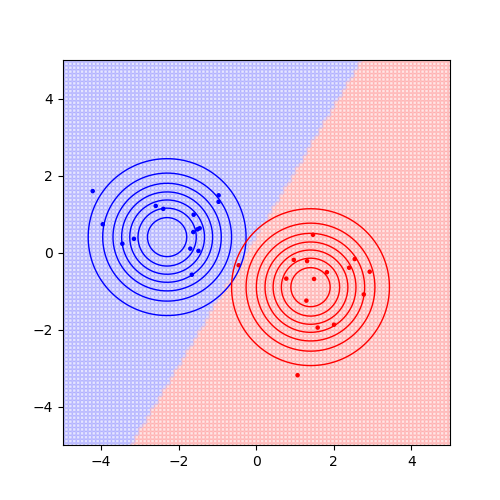
\includegraphics[scale=0.7]{Section_3/GDA.png}
    \caption{GDA of Data Generated from 2 Gaussisans centered at $(-2.3, 0.4)$ and $(1.4, -0.9)$ with unit covariance. The decision boundary is slightly off since MLE approximates the true means. }
    \label{fig:enter-label}
\end{figure}

\section{K Nearest Neighbors}      

Given a bunch of points in a metric space $(\mathcal{X}, d)$ that have classification labels, we want to label new datapoints $\hat{\mathbf{x}}$ based on the labels of other points that already exist in our dataset. One way to look at it is to look for close points within the dataset and use their labels to predict the new ones. 

\begin{definition}
Given a dataset $\mathcal{D} = \{\mathbf{x}^{(i)}, \mathbf{y}^{(i)}\}$ and a point $\hat{\mathbf{x}} \in (\mathcal{X}, d)$, let the \textbf{k closest neighborhood} of $\hat{\mathbf{x}}$ be $N_k (\hat{\mathbf{x}}) \subset [N]$ defined as the indices $i$ of the $k$ points in $\mathcal{D}$ that is closest to $\hat{\mathbf{x}}$ with respect to the distance metric $d_\mathcal{X}$. 
\end{definition}

\begin{definition}[K Nearest Neighbors]
The \textbf{K Nearest Neighbors (KNN)} is a discriminative nonparametric supervised learning algorithm that doesn't have a training phase. Given a new point $\hat{\mathbf{x}}$, we look at all points in its k closest neighborhood, and $h(\hat{\mathbf{x}})$ will be equal to whatever the majority class will be in. Let us one-hot encode the labels $\mathbf{y}^{(i)}$ into $\mathbf{e}_i$'s, and the number of data point in the $i$th class can be stored in the variable 
\[a_i = \sum_{i \in N_k (\hat{\mathbf{x}})} 1_{\{\mathbf{y}^{(i)} = \mathbf{e}_i\}}\]
which results in the vector storing the counts of labels in the k closest neighborhood 
\[\mathbf{a} = (a_1, a_2, \ldots, a_\mathcal{K}) = \bigg( \sum_{i \in N_k (\hat{\mathbf{x}})} 1_{\{\mathbf{y}^{(i)} = \mathbf{e}_1\}}, \sum_{i \in N_k (\hat{\mathbf{x}})} 1_{\{\mathbf{y}^{(i)} = \mathbf{e}_2\}}, \ldots, \sum_{i \in N_k (\hat{\mathbf{x}})} 1_{\{\mathbf{y}^{(i)} = \mathbf{e}_\mathcal{K}\}} \bigg)  \]
and take the class with the maximum element as our predicted label. 
\end{definition}

The best choice of $K$ depends on the data: 
\begin{enumerate}
    \item Larger values of $K$ reduces the effect of noise on the classification, but make boundaries between classes less distinct. The number of misclassified data points (error) increases. 
    \item Smaller values are more sensitive to noise, but boundaries are more distinct and the number of misclassified data points (error) decreases.
\end{enumerate}
Too large of a $K$ value may increase the error too much and lead to less distinction in classification, while too small of a k value may result in us overclassifying the data. Finally, in binary (two class) classification problems, it is helpful to choose $K$ to be odd to avoid tied votes.

This is an extremely simple algorithm that may not be robust. For example, consider $K \geq 3$, and we are trying to label a point $\hat{\mathbf{x}}$ that happens to be exactly where one point is on our dataset $\mathbf{x}^{(i)}$. Then, we should do $h(\hat{\mathbf{x}}) = y^{(i)}$, but this may not be the case if there are no other points with class $y^{(i)}$ in the k closest neighborhood of $\mathbf{x}^{(i)}$. Therefore, we want to take into account the distance of our new points from the others. 

\begin{definition}[Weighted Nearest Neighbor Classifier]
Let us define a monotinically decreasing function $\omega: \mathbb{R}_0^+ \mapsto \mathbb{R}_0^+$. Given a point $i \in N_k (\hat{\mathbf{x}})$, we can construct the weight of our matching label as inversely proportional to the distance: $\omega_i [ d(\hat{\mathbf{x}}, \mathbf{x}^{(i)})]$ and store them as 
\[\mathbf{a} = (a_1, a_2, \ldots, a_\mathcal{K}) = \bigg( \sum_{i \in N_k (\hat{\mathbf{x}})} \omega_i 1_{\{\mathbf{y}^{(i)} = \mathbf{e}_1\}}, \sum_{i \in N_k (\hat{\mathbf{x}})} \omega_i 1_{\{\mathbf{y}^{(i)} = \mathbf{e}_2\}}, \ldots, \sum_{i \in N_k (\hat{\mathbf{x}})} \omega_i 1_{\{\mathbf{y}^{(i)} = \mathbf{e}_\mathcal{K}\}} \bigg)  \]
and again take the class with the maximum element. 
\end{definition}

One caveat of KNN is in high dimensional spaces, as its performance degrades quite badly due to the curse of dimensionality. 

\begin{example}[]
    Consider a dataset of $N$ samples uniformly distributed in a $d$-dimensional hypercube. Now given a point $x \in [0, 1]^d$, we want to derive the expected radius $r_k$ required to encompass its $k$ nearest neighbors. Let us define this ball to be $B_{r_k} \coloneqq \{ z \in \mathbb{R}^d \mid ||z - x ||_2 \leq r_k \}$. Since thse $N$ points are uniformly distributed, the expected number of points contained in $B_{r_k} (x)$ is simply the proportion of the volume that $B_{r_k} (x)$ encapsulates in the box, multiplied by $N$. Therefore, for some fixed $x$ and $r$, let us denote $Y(x, y)$ as the random variable representing the number of points contained within $B_r (x)$. By linearity of expectation and summing over the expectation for whether each point will be in the ball, we have 
    \[\mathbb{E}[Y (x, r)] = N \cdot \frac{\mu(B_r (x) \cap [0, 1]^d) }{\mu([0, 1]^d)}\]
    where $\mu$ is the Lebesgue measure of $\mathbb{R}^d$. Let us assume for not that we don't need to worry about cases where the ball is not fully contained within the cube, so we can just assume that $Y$ is only dependent on $r$: $Y(r)$. Also, since the volume of the hypercube is $1$,  $\mu([0, 1]^d) = 1$ and we get 
    \[\mathbb{E}[Y(r)] = N \cdot C_d \cdot r^d\]
    which we set equal to $k$ and evaluate for $r$. $C_d$ is a constant such that the volume of the hypersphere of radius $r$ can be derived as $V = C_d \cdot r^d$. We therefore get 
    \[N \cdot C_d \cdot r_k^d = k \implies r_k = \bigg( \frac{k}{N C_d} \bigg)^{1/d}\]
    It turns out that $C_d$ decreases exponentially, so the radius $r_k$ explodes as $d$ grows. Another way of looking at this is that in high dimensions, the $\ell_2$ distance between all the pairwise points are close in every single dimension, so it becomes harder to distinguish points that are close vs those that are far.  
\end{example} 

\section{Decision Trees}

\begin{definition}[Decision Trees]
Like K nearest neighbors, \textbf{decision trees} are discriminative nonparametric classification algorithms that involves creating some sort of tree that represents a set of decisions using a given set of input data $\mathbf{x}^{(i)}$ with its given classification $\mathbf{y}^{(i)}$. When predicting the class of a new input $\hat{\mathbf{x}}$, we would look at its attributes in some order, e.g. $\hat{x_1}, \hat{x}_2, \hat{x}_3$, and make a decision on which class it is in. 
\begin{center}
    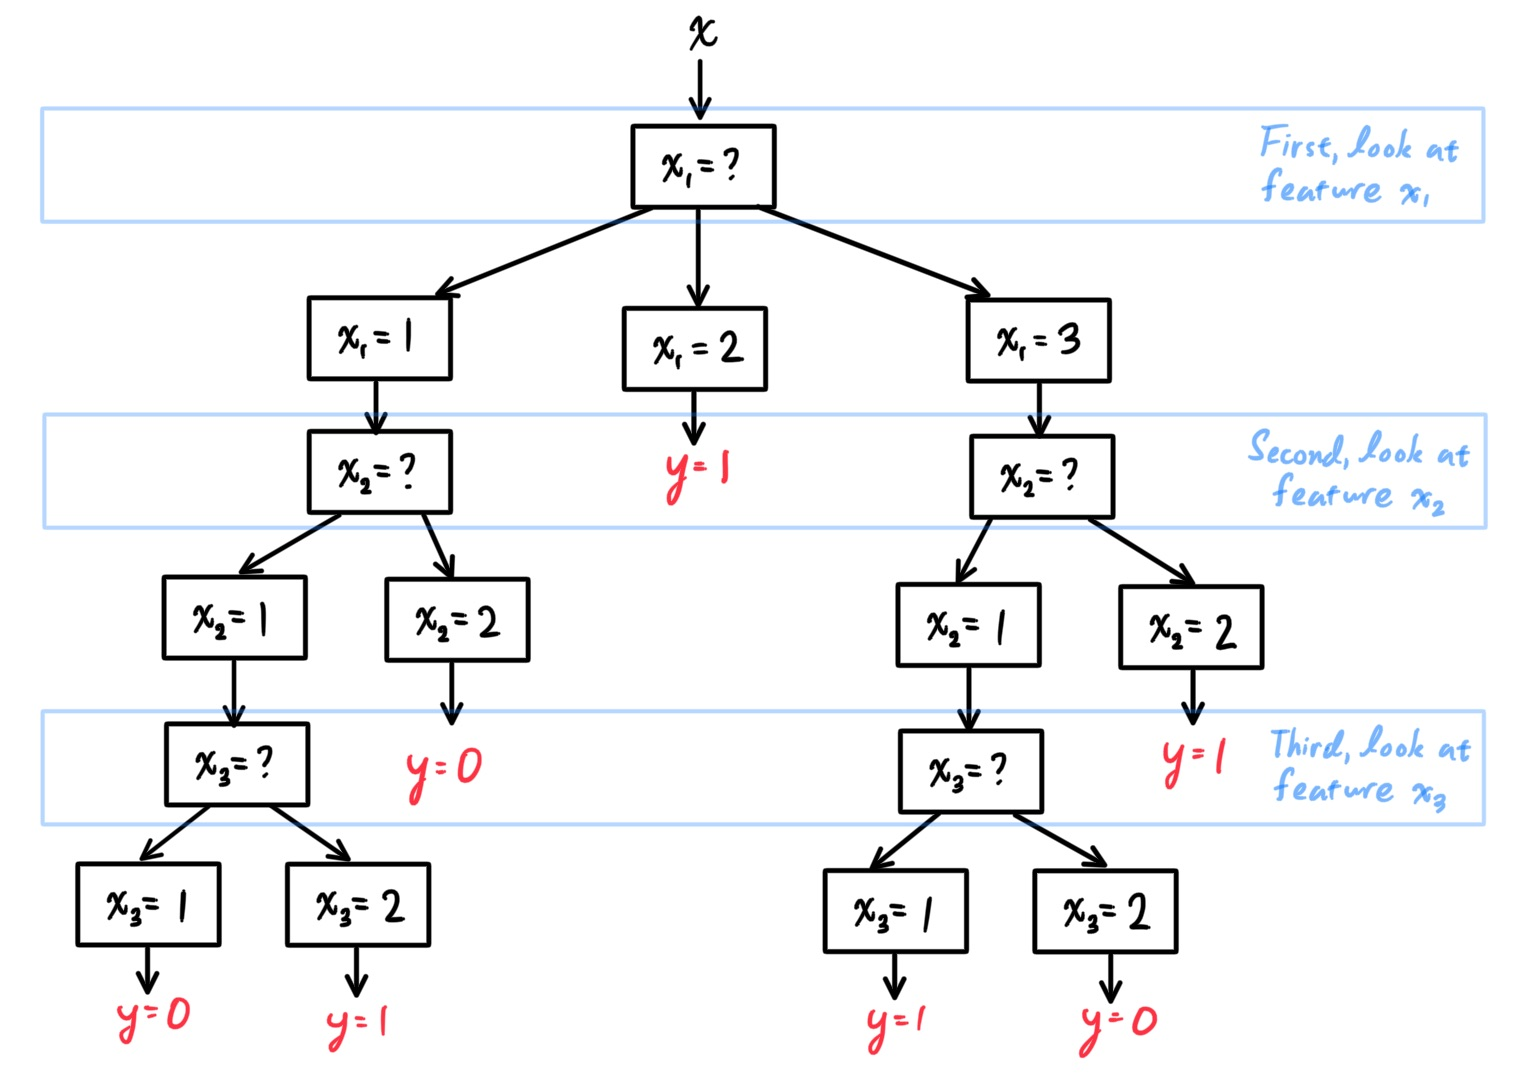
\includegraphics[scale=0.2]{general_decision_tree.jpg}
\end{center}
The decision tree tries to take advantage of some nontrivial covariance between $X$ and $Y$ by constructing nested partitions of the dataset $\mathcal{D}$, and within a partition, it predicts the label that comprises the majority. 
\end{definition}

For now, let us assume that $\mathcal{X}$ is a Cartesian product of discrete sets, and we will extend them to continuous values later. Let us look at an example to gain some intuition. 

\begin{example}
Consider the dataset 
\begin{center}
    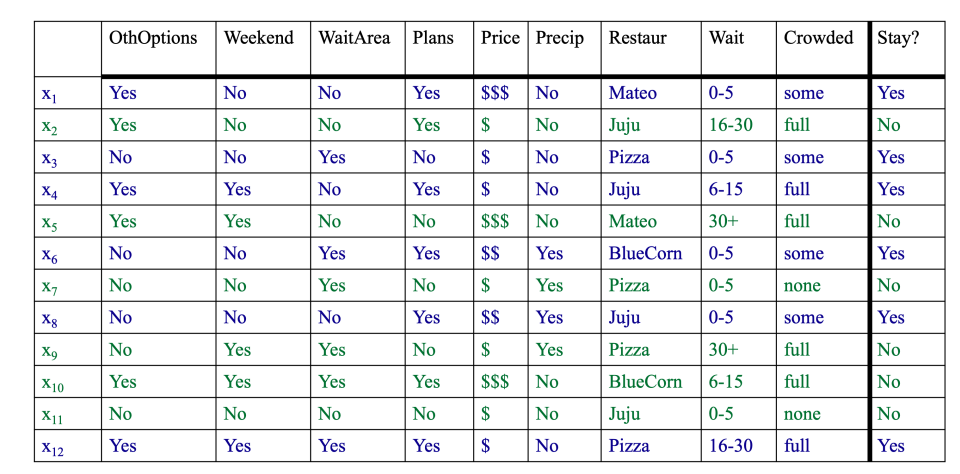
\includegraphics[scale=0.4]{decision_data.png}
\end{center}
Let us denote $\mathcal{D}$ as the dataset, and say that $F_1, \ldots, F_d$ were the features. This is a binary classification problem, and we can count that there are $6$ positives and $6$ negative labels. 
\end{example}

The simplest decision tree is the trivial tree, with one node that predicts the majority of the dataset. In this case, the data is evenly split, so without loss of generality we will choose $h_0 (\mathbf{x}) = 1$. We want to quantify how good our model is, and so like always we use a loss function. 

\subsection{Splitting Criteria}

Just like how a linear model is completely defined by its parameter $\boldsymbol{\theta}$, a decision tree is completely defined by the sequences of labels that it splits on. Therefore, training this is equivalent to defining the sequence, but we can't define this sequence unless we can compare how good a given decision tree is, i.e. unless we have defined a proper loss function. Depending on the training, we can use a greedy algorithm or not, and we have the flexibility to choose whether or not we can split on the same feature multiple times. 

\subsubsection{Misclassification Error}

\begin{definition}[Musclassification Error]
We will simply use the misclassification loss function. 
\[L(h; \mathcal{D}) = \frac{1}{N} \sum_{i=1}^N 1_{\{y^{(i)} \neq h(x^{(i)})\}} = 1 - \text{accuracy}\]
Minimizing this maximizes the accuracy, so this is a reasonable one to choose. How do we train this? Unlike regression, this loss is not continuous, so the gradient is $0$, and furthermore the model isn't even parametric, so there are no gradients to derive! 
\end{definition}

Fortunately, the nature of the decision tree only requires us to look through the explanatory variables $x_1, \ldots, x_n$ and decide which one to split. 

\subsubsection{Information Gain}

Let us take a decision tree $h$ and model the accuracy of it as a random variable: $1_{\{Y = h_0 (X)\}} \sim \mathrm{Bernoulli}(p)$, where $p$ is the accuracy. A higher accuracy of $h$ corresponds to a lower entropy, and so the entropy of the random variable is also a relevant indicator. 
\[H(1_{\{Y = h_0 (X)\}}) = p \log{p} + (1 - p) \log(1 - p)\]
Therefore, when we are building a tree, we want to choose the feature $x_i$ to split based on how much it lowers the entropy of the decision tree. 

To set this up, let us take our dataset $\mathcal{D}$ and set $X_i$ as the random variable representing the distribution (a multinomial) of the $x_i^{(j)}$'s, and $Y$ as the same for the $y^{(j)}$'s. This is our maximum likelihood approximation for the marginalized distribution of the joint measure $X \times Y = X_1 \times \ldots \times X_D \times Y$. 

Given a single node, we are simply going to label every point to be whatever the majority class is in $\mathcal{D}$. Therefore, we start off with the entropy of our trivial tree $H(Y)$. Then, we want to see which one of the $X_d$ features to split on, and so we can compute the conditional entropy $H(Y, X_d)$ to get the information gain $I(Y; X_d) = H(Y) - H(Y \mid X_d)$ for all $d = 1, \ldots, D$. We want to find a feature $X_d$ that maximize this information gain, i.e. decreases the entropy as much as possible (a greedy algorithm), and we find the next best feature (with or without replacement), so that we have a decreasing sequence. 
\[H(X) \geq H(X ; Y) \geq H(X ; Y, Z) \geq H(X ; Y, Z, W) \geq \ldots \geq 0\]

\begin{example}
Continuing the example above, since there are $6$ labels of $0$ and $1$ each, we can model this $Y \sim \mathrm{Bernoulli}(0.5)$ random variable, with entropy 
\[H(Y) = \mathbb{E}[-\log_2 p(Y)] = \frac{1}{2} \big( -\log_2 \frac{1}{2} \big) + \frac{1}{2} \big( -\log_2 \frac{1}{2} \big) = 1\]
Now what would happen if we had branched according to how crowded it was, $X_{\mathrm{crowded}}$. Then, our decision tree would split into 3 sections: 
\begin{center}
    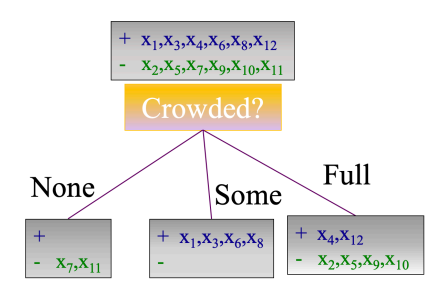
\includegraphics[scale=0.5]{decision_crowded.png}
\end{center}
In this case, we can define the multinomial distribution $X_{\mathrm{crowded}}$ representing the proportion of the data that is crowded in a specific level. That is, $X_{\mathrm{crowded}} \sim \mathrm{Multinomial}(\frac{2}{12}, \frac{4}{12}, \frac{6}{12} \big)$, with 
\[\mathbb{P}(X_{\mathrm{crowded}} = x) = \begin{cases} 2/12 & \text{ if } x = \text{ none} \\ 4/12 & \text{ if } x = \text{ some} \\ 6/12 & \text{ if } x = \text{ full} \end{cases} \]
Therefore, we can now compute the conditional entropy of this new decision tree conditioned on how crowded the store is 
\begin{align*}
    H(Y \mid X_{\mathrm{crowded}}) & = \sum_x \mathbb{P}(X_{\mathrm{crowded}} = x) H(Y \mid X_{\mathrm{crowded}} = x) \\
    & = \frac{2}{12} H(\mathrm{Bern}(1)) + \frac{4}{12} H(\mathrm{Bern}(0)) + \frac{6}{12} H(\mathrm{Bern}(1/3)) = 0.459 \\
    I(Y; X_{\mathrm{crowded}}) & = 0.541
\end{align*}
We would do this for all the features and greedily choose the feature that maximizes our information gain. 
\end{example}

\begin{example}
The Ferrari F1 team hired you as a new analyst! You were given the following table of the past race history of the team. You were asked to use information gain to build a decision tree to predict race wins. First, you will need to figure out which feature to split first. 

\begin{center}
\begin{tabular}[c]{c|c|c||c}
Rain & Good Strategy & Qualifying & Win Race \\ \hline
1 & 0 & 0 & 0 \\
1 & 0 & 0 & 0 \\
1 & 0 & 1 & 0 \\
0 & 0 & 1 & 1 \\
0 & 0 & 0 & 0 \\
0 & 1 & 1 & 1 \\
1 & 0 & 1 & 0 \\
0 & 1 & 0 & 1 \\
0 & 0 & 1 & 1 \\
0 & 0 & 1 & 1 \\
\end{tabular}
\end{center}
Let $X \sim \mathrm{Bernoulli}(1/2)$ be the distribution of whether a car wins a race over the data. Then its entropy is 
\[H(X) = \mathbb{E}[-\log_2 p(x)] = \frac{1}{2} \big( -\log_2 \frac{1}{2} \big) + \frac{1}{2} \big( -\log_2 \frac{1}{2} \big) = 1\]
Let $R \sim \mathrm{Bernoulli}(4/10), G \sim \mathrm{Bernoulli}(2/10), Q \sim \mathrm{Bernoulli}(6/10)$ be the distribution of the features rain, good strategy, and qualifying over the data, respectively. Then, the conditional entropy of $X$ conditioned on each of these random variables is 
\begin{align*}
    H(X \mid R) & = \mathbb{P}(R = 1)\, H(X \mid R = 1) + \mathbb{P}(R = 0) \, H(X \mid R = 0) \\
    & = \frac{4}{10} \cdot - \big( 1 \cdot \log_2 1 + 0 \cdot \log_2 0 \big) + \frac{6}{10} \cdot - \big( \frac{1}{6} \cdot \log_2 \frac{1}{6} + \frac{5}{6} \cdot \log_2 \frac{5}{6} \big) \approx 0.390 \\
    H(X \mid G) & =  \mathbb{P}(G = 1)\, H(X \mid G = 1) + \mathbb{P}(G = 0) \, H(X \mid G = 0) \\
    & = \frac{2}{10} \cdot - \big( 1 \cdot \log_2 1 + 0 \cdot \log_2 0 \big) + \frac{8}{10} \cdot - \big( \frac{3}{8} \cdot \log_2 \frac{3}{8} + \frac{5}{8} \log_2 \frac{5}{8} \big) \approx 0.763\\
    H(X \mid Q ) & = \mathbb{P}(Q = 1)\, H(X \mid Q = 1) + \mathbb{P}(Q = 0) \, H(X \mid Q = 0) \\
    & = \frac{6}{10} \cdot - \big( \frac{4}{6} \cdot \log_2 \frac{4}{6} + \frac{2}{6} \cdot \log_2 \frac{2}{6} \big) + \frac{4}{10} \cdot - \big( \frac{1}{4} \log_2 \frac{1}{4} + \frac{3}{4} \log_2 \frac{3}{4} \big) \approx 0.875
\end{align*}
Therefore, the information gain are 
\begin{align*}
    I(X; R) & = 1 - 0.390 = 0.610 \\
    I(X; G) & = 1 - 0.763 = 0.237 \\
    I(X; Q) & = 1 - 0.875 = 0.125 
\end{align*}
And so I would split on $R$, the rain, which gives the biggest information gain. 
\end{example}

\subsubsection{Gini Index}

Finally, we can use the Gini index of $X \sim \mathrm{Bernoulli}(p)$, defined 
\[G(X) = 2 p (1 - p)\]


\begin{example}
We do the same as the Ferrari example above but now with the Gini reduction. 

Let $X \sim \mathrm{Bernoulli}(1/2)$ be the distribution of whether a car wins a race over the data. Then its Gini index, which I will label with $\mathcal{G}$, is \[\mathcal{G} (X) = 2 \cdot \frac{1}{2} \cdot \frac{1}{2} = \frac{1}{2}\]
Let $R \sim \mathrm{Bernoulli}(4/10), G \sim \mathrm{Bernoulli}(2/10), Q \sim \mathrm{Bernoulli}(6/10)$ be the distribution of the features rain, good strategy, and qualifying over the data, respectively. Then we compute the conditional expectation 
\begin{align*}
    \mathbb{E}[\mathcal{G}(X \mid R)] & = \mathbb{P}(R = 1)\, \mathcal{G}(X \mid R = 1) + \mathbb{P}(R = 0) \, \mathcal{G}(X \mid R = 0) \\ 
    & = \frac{4}{10} \bigg[ 2 \cdot \frac{4}{4} \cdot \frac{0}{4} \bigg] + \frac{6}{10} \bigg[ 2 \cdot \frac{1}{6} \cdot \frac{5}{6} \bigg] \approx 0.167 \\
    \mathbb{E}[\mathcal{G}(X \mid G)] & = \mathbb{P}(G = 1)\, \mathcal{G}(X \mid G = 1) + \mathbb{P}(G = 0) \, \mathcal{G}(X \mid G = 0) \\ 
    & = \frac{2}{10} \bigg[ 2 \cdot \frac{2}{2} \cdot \frac{0}{2} \bigg] + \frac{8}{10} \bigg[ 2 \cdot \frac{3}{8} \cdot \frac{5}{8} \bigg] \approx 0.375 \\
    \mathbb{E}[\mathcal{G}(X \mid Q)] & = \mathbb{P}(Q = 1)\, \mathcal{G}(X \mid Q = 1) + \mathbb{P}(Q = 0) \, \mathcal{G}(X \mid Q = 0) \\ 
    & = \frac{6}{10} \bigg[ 2 \cdot \frac{4}{6} \cdot \frac{2}{6} \bigg] + \frac{4}{10} \bigg[ 2 \cdot \frac{1}{4} \cdot \frac{3}{4} \bigg] \approx 0.417
\end{align*}
Therefore, the Gini reduction, which I'll denote as $I_{\mathcal{G}}$, is 
\begin{align*}
    I_{\mathcal{G}} (X ; R) & = 0.5 - 0.167 = 0.333 \\
    I_{\mathcal{G}} (X ; G) & = 0.5 - 0.375 = 0.125 \\
    I_{\mathcal{G}} (X ; Q) & = 0.5 - 0.417 = 0.083
\end{align*}
Since branching across the feature $R$, the rain, gives the biggest Gini reduction, we want to split on the rain feature first. 
\end{example}


\subsection{Regularization}

Given a dataset with $D$ binary features, let $g(H, D)$ be the number of binary trees with depth at most $H$ (including root node), with the restriction that the trees may not split on some variable multiple times within a path to a leaf node. Then, $g$ can be defined recursively. 
\begin{enumerate}
    \item First, if $H = 1$, then $g(H, D) = 1$ always since we are just creating the trivial binary tree of one node. 
    \item If $D = 0$, then there are no features to split on and therefore we just have the single node $g(H, D) = 1$. 
    \item If $H > 1$ and $D > 0$, then say that we start with a node. We can either make this a leaf node by not performing any splitting at all, or split on one of the $D$ variables. Then for each of the 2 nodes created on the split, we are now working with $D-1$ features and a maximum height of $H-1$ for each of the subtrees generated from the 2 nodes. 
\end{enumerate}
All this can be expressed as 
\[g(H, D) = \begin{cases} 1 + D \, \big[ g(H - 1, D - 1) \big]^2 & \text{ if } H > 1, D > 0 \\ 1 & \text{ if } H = 1 \text{ or } D = 0 \end{cases} \]
which is extremely large (in fact, NP hard). Therefore, some tricks like regularization must be implemented to limit our search space. 

By defining the complexity of our decision tree $\Omega(h)$ as the number of nodes within the tree, we can modify our objective function to 
\[L(h; \mathcal{D}) = \frac{1}{N} \sum_{i=1}^N 1_{\{y^{(i)} \neq h(x^{(i)})\}} + \lambda \Omega(h)\]
We can impose this constraint directly on the training algorithm, or we can calculate the regularized loss after the tree has been constructed, which is a method called \textbf{tree pruning}. 

Given a large enough $\lambda$, we can in fact greatly reduce our search space by not considering any trees further than a certain point. 

\begin{theorem}
We describe a tree as a set of leaves, where leaf $k$ is a tuple containing the logical preposition satisfied by the path to leaf $k$, denoted $p_k $, and the class label predicted by the leaf, denoted $\hat{y}_k$. For a dataset with $d$ binary features, $p_k: \{0, 1\}^d \to \{0, 1\}$ is a function that returns $1$ if a sample $x_i$ satisfies the preposition, and $0$ otherwise. That is, leaf $k$ is $(p_k, \hat{y}_k),$ and a tree $f$ with $K$ leaves is described as a set $f = \{(p_1, \hat{y}_1), \hdots, (p_K, \hat{y}_K)\}$. Assume that the label predicted by $\hat{y}_k$ is always the label for the majority of samples satisfying $p_k$. Finally, let $m_k = \sum_{i=1}^n p_k(x_i)$ denote the number of training samples ``captured'' by leaf $k$.

Given a (potentially optimal) tree $$f = \{(p_1, \hat{y}_1), \hdots, (p_{\kappa}, \hat{y}_{\kappa}), \hdots, (p_K, \hat{y}_K)\},$$ 
the tree $f' = \{(p_1, \hat{y}_1), \hdots, (p_{\kappa_1}, \hat{y}_{\kappa_1}), (p_{\kappa_2}, \hat{y}_{\kappa_2}), \hdots, (p_K, \hat{y}_K)\}$ 
produced by splitting leaf $(p_{\kappa}, \hat{y}_{\kappa})$ into two leaves $(p_{\kappa_1}, \hat{y}_{\kappa_1})$ and $(p_{\kappa_2}, \hat{y}_{\kappa_2})$ and any tree produced by further splitting $(p_{\kappa_1}, \hat{y}_{\kappa_1})$ or $(p_{\kappa_2}, \hat{y}_{\kappa_2})$ cannot  be optimal if $m_{\kappa} < 2n\lambda$.
\end{theorem}
\begin{proof}
Let $c$ be the number of misclassifications in leaf $(p_{\kappa}, \hat{y}_{\kappa})$. Since a leaf classifies according to the majority of $m_{\kappa}$, we must have 
\[c \leq \frac{m_\kappa}{2} < n \lambda\]
By splitting leaf $(p_\kappa, \hat{y}_\kappa)$ into leaves $(p_{\kappa_1}, \hat{y}_{\kappa_1})$ and $(p_{\kappa_2}, \hat{y}_{\kappa_2})$, assume that we have reduced the number of misclassifications by $b \leq c$. Then, we have 
\[\ell(f^\prime, \mathbf{X}, \mathbf{y}) = \ell(f, \mathbf{X}, \mathbf{y}) - \frac{b}{n}\]
However, we have increased the number of leaves by $1$, and so 
\[\lambda s(f^\prime) = \lambda s(f) + \lambda\]
Combining the last two equations, we have obtained 
\[R (f^\prime, \mathbf{X}, \mathbf{y}) = R(f, \mathbf{X}, \mathbf{y}) + \lambda - \frac{b}{n}\]
However, we know that 
\begin{align*}
    b \leq c & \implies \frac{b}{n} \leq \frac{c}{n} < \frac{n \lambda}{n} = \lambda \\
    & \implies - \frac{b}{n} > - \lambda \\
    & \implies \lambda - \frac{b}{n} > \lambda - \lambda = 0
\end{align*}
and so $R (f^\prime, \mathbf{X}, \mathbf{y}) > R(f, \mathbf{X}, \mathbf{y})$. This means that $f^\prime$ cannot be optimal according to our regularized objective. We have also proved that further splitting $(p_{\kappa_1}, \hat{y}_{\kappa_1})$ or $(p_{\kappa_2}, \hat{y}_{\kappa_2})$ cannot  be optimal since we can just set $f = f^\prime$, and apply the same argument. 
\end{proof}

\subsection{Splitting on Continuous Values}



\subsection{Random Forests}
A decision tree is our first example of a supervised model that is both interpretable yet nonlinear. 


\subsection{Boosting}



Discriminative Model

\section{Kernel Methods} 

Let $\mathcal{H}$ be the $\ell_2$ Hilbert space of real-valued measurable functions over $X$. Then, for a given $x \in X$, we can define the \textbf{Dirac evaluation functional} $\delta_x$, which is a linear functional living in the dual $\mathcal{H}^\ast$ defined 
\[\delta_x f = f(x)\]
We will take it for granted (as it is too technical to prove for now) that $\delta_x$ is bounded in the way such that for all $x \in X$ and $f \in \mathcal{H}$, we have 
\[|f(x)| \leq M ||f||_2 \]
So by Reisz representation theorem we have a natural isomorphism $\gamma: X^\ast \rightarrow X$, defined 
\[\delta_x f = f(x) = \langle f, k_x \rangle_{\mathcal{H}}\]
Now since $k_x$ is itself a function defined over $X$, we have for any $y \in X$, 
\[k_x (y) = \delta_y k_x = \langle k_x, k_y \rangle_{\mathcal{H}}\]
where $k_y$ is the representative of $\delta_y$. This allows us to define the \textbf{reproducing kernel} $K: X \times X \rightarrow \mathbb{R}$ over $\mathcal{H}$ as 
\[K(x, y) = \langle k_x, k_y \rangle_{\mathcal{H}}\]


\begin{definition}[Reproducing Kernel Hilbert Space]
    A \textbf{reproducing kernel hilbert space (RKHS)}
\end{definition}


Let us state some properties. 

\begin{definition}[Positive Definite Function]
    A symmetric function $K$ is positive definite if for any $L_2$ function $f$ (other than the $0$ function), we have 
    \[\int_{X \times X} f(x) K(x, y) f(y) \,dx \,dy > 0\]
    This generalizes the definition for matrices since defined over a finite subset of $X$, $K$ reduces to a matrix $\mathcal{K}$ defined as $(\mathcal{K})_{ij} = K(x_i, x_j)$ is positive definite. 
\end{definition}

\begin{theorem} 
   All reproducing kernels are positive definite.  
\end{theorem} 

This is easy to prove, but the converse is highly nontrivial. 

\begin{theorem}[Moore-Aronszajn] 
   Any positive definite function $K$ is a reproducing kernel for some RKHS.  
\end{theorem} 
\begin{proof} 
    We won't be too rigorous about this since this is not a functional analysis course. Assume that we have a positive definite kernel $K: X \times X \rightarrow \mathbb{R}$, where $X$ is some measurable set, and we will show how to make a RKHS $\mathcal{H}_k$ such that $K$ is the reproducing kernel on $\mathcal{H}$. It turns out that $\mathcal{H}_k$ is unique up to isomorphism. Since $X$ exists, let us first define the set $S = \{ k_x \mid x \in X\}$ such that $k_x (y) \coloneqq K(x, y)$. Now let us define the vector space $V$ to be the span of $S$. Therefore, each element $v \in V$ can be written as 
    \[v = \sum_i \alpha_i k_{x_i}\]
    Now we want to define an inner product on $V$. By expanding out the vectors w.r.t. the basis and the properties of bilinearity, we have 
    \[\langle k_x, k_y \rangle_{V} = \bigg\langle \sum_i \alpha_i k_{x_i} , \sum_i \beta_i k_{y_i} \bigg\rangle = \sum_{i, j} \alpha_i \beta_j K(x_i, y_j)\] 
    At this point, $V$ is not necessarily complete, but we can force it to be complete by taking the limits of all Cauchy sequences and adding them to $V$. In order to complete the construction, we need to ensure that $K$ is continuous and doesn't diverge, i.e. 
    \[\iint K^2 (x, y) \,dx\,dy < +\infty\]
    which is a property known as finite trace. Too much to write down here at this point, but for further information look at $\href{http://users.umiacs.umd.edu/~hal/docs/daume04rkhs.pdf}{the article here}$. 
\end{proof}


\section{Support Vector Machines}

A support vector machine focuses only on the points that are most difficult to tell apart, whereas other classifiers pay attention all of the points. A SVM is a discriminative, non-probabilistic model. Let us first assume that our dataset $\mathcal{D} = \{\mathbf{x}_i, y_i\}$ is linearly separable with $y_i \in \{-1, +1\}$. Based on previous algorithms like the perceptron, it will find some separating hyperplane. However, there's an infinite number of separating hyperplanes as shown in Figure \ref{fig:svm_intro}. What support vector machines want to do is to find the best one, with the ``best" defined as the hyperplane that maximizes the distance between either the closest positive or negative samples, shown in Figure $\ref{fig:svm_intro2}$.  

\begin{figure}[hbt!] 
    \centering 
    \begin{subfigure}[b]{0.45\textwidth} 
        \centering 
        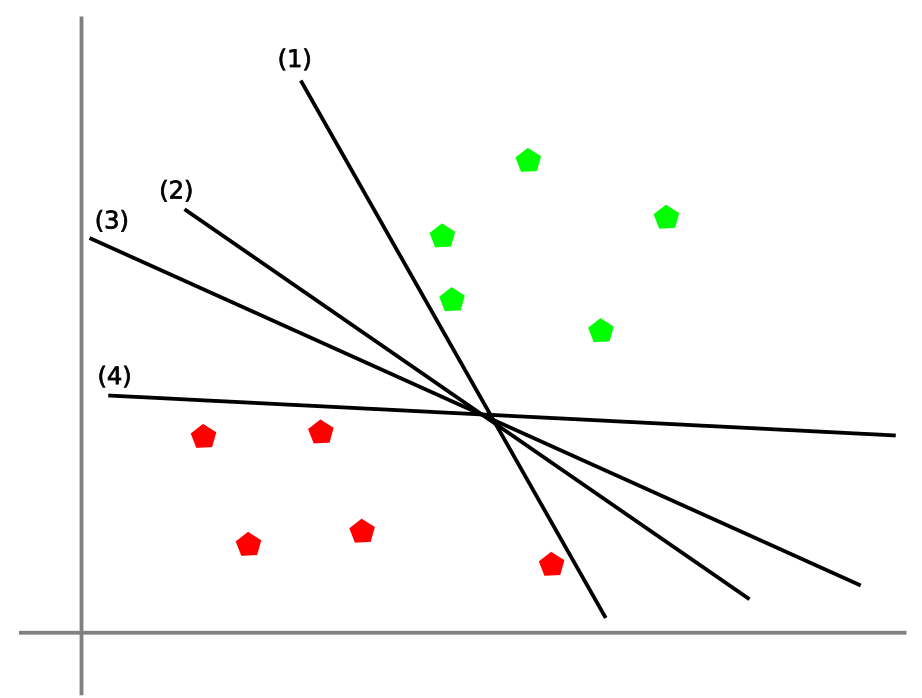
\includegraphics[width=\textwidth]{svm_intro.png} 
        \caption{Planes such as (1) and (4) are ``too close" to the positive and negative samples. } 
        \label{fig:svm_intro}
    \end{subfigure}
    \hfill
    \begin{subfigure}[b]{0.45\textwidth} 
        \centering 
        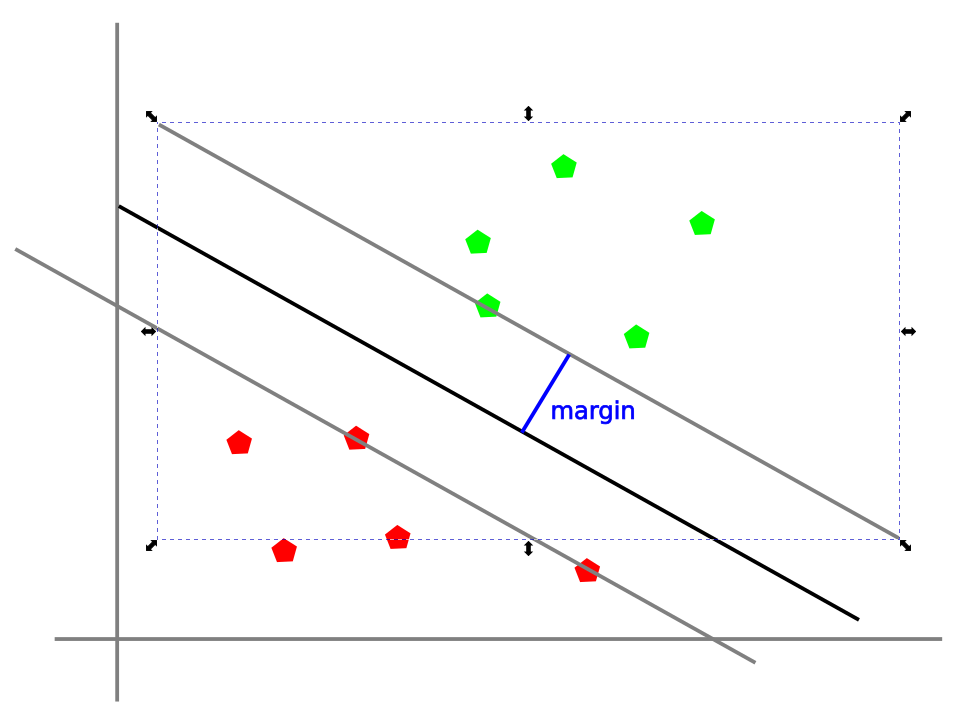
\includegraphics[width=\textwidth]{svm_intro_2.png}  
        \caption{SVMs try to find the separating hyperplane with the best minimum margin.} 
        \label{fig:svm_intro2}
    \end{subfigure} 

    \caption{} 
    \label{} 
\end{figure}

We want to formalize the concepts of these margins that we wish to maximize. To do this, we will define two terms. 

\begin{definition}[Geometric margin]
    Given a point $\mathbf{x}_0$ and a hyperplane of equation $\mathbf{w} \cdot \mathbf{x} + b = 0$, the distance from $\mathbf{x}_0$ to the hyperplane, known as the \textbf{geometric margin}, can be computed with the formula 
    \begin{equation*}
        d = \frac{|\mathbf{x}_0 \cdot \mathbf{w} + b|}{||\mathbf{w}||}  
    \end{equation*} 
    Therefore, the geometric margin of the $i$th sample with respect to the hypothesis $f$ is defined 
    \begin{equation*}
        \gamma_i = \frac{y_i \, (\mathbf{w} \cdot \mathbf{x}_i + b)}{||\mathbf{w}||} 
    \end{equation*} 
\end{definition}

We wish to optimize the parameters $\mathbf{w}, b$ in order to maximize the minimum of the geometric margins (the distance between the closest point and the hyperplane). 
\begin{equation*}
  \argmax_{\mathbf{w}, b} \min_i \gamma_i = \argmax_{\mathbf{w}, b} \bigg\{ \frac{1}{||\mathbf{w}||} \min_i \big[y_i \, (\mathbf{w} \cdot \mathbf{x}_i + b) \big] \bigg\}
\end{equation*}

Direct solution of this optimization problem would be very complex, and so we convert this into an equivalent problem that is much easier to solve. Note that the solution to the above term is not unique. If there was a solution $(\mathbf{w}^\ast, b^\ast)$, then 
\begin{equation*}
    \frac{y_i (\mathbf{w} \cdot \mathbf{x}_i + b)}{||\mathbf{w}||} = \frac{y_i (\lambda \mathbf{w} \cdot \mathbf{x}_i + \lambda b)}{||\lambda \mathbf{w}||}  
\end{equation*}
That is, the geometric margin is not sensitive to scaling of the parameters of the hyperplane. Therefore, we can scale the numerator and the denominator by whatever we want and use this freedom to set 
\begin{equation*}
    y_i ( \mathbf{w} \cdot \mathbf{x}_i + b ) = 1 
\end{equation*}
for the point that is closest to the surface. In that case, all data points will satisfy the constraints 
\begin{equation*}
    y_n (\mathbf{w} \cdot \mathbf{x}_i + b) \geq 1
\end{equation*}
In the case of data points for which the equality holds, the constraints are said to be \textit{active}, whereas for the remainder they are \textit{inactive}. Therefore, it will always be the case that $\min_i \big[ y_i \, (\mathbf{w} \cdot \mathbf{x}_i + b)\big] = 1$, and the constraint problem reduces to 
\begin{equation*}
    \argmax_{\mathbf{w}, b} \frac{1}{||\mathbf{w}||} = \argmin_{\mathbf{w}, b} \frac{1}{2} ||\mathbf{w}||^2 \text{ subject to constraints } y_i (\mathbf{w} \cdot \mathbf{x}_i + b) \geq 1 
\end{equation*}
This final step is the most significant step in this derivation and may be hard to wrap around the first time. So we dedicate the next subsubsection for this. 


\subsubsection{Functional and Geometric Margins} 


We could just work straight with this geometric margin, but for now, let's try to extend what we did with the perceptron into SVMs. We will find out that extending the concept of functional margins into SVMs leads to ill-defined problems. In the perceptron, we wanted to construct a function $f(\mathbf{x}) = \mathbf{w} \cdot \mathbf{x} + b$ such that 
\begin{equation*}
    y_i \, f(\mathbf{x}_i) \geq 0 \text{ for all } i = 1, 2, \ldots, N
\end{equation*}

\begin{definition}[Functional Margin]
  The value of $y_i \, f(\mathbf{x}_i)$ gives us our confidence on our classification, and in a way it represents a kind of distance away from the separating hyperplane (if this value was $0$, then we would be 50 50 split on whether to label it positive or negative). Therefore, we shall define 
  \begin{equation*}
      \hat{\gamma}_i  & = y_i f(\mathbf{x}_i) 
  \end{equation*}
as the \textbf{functional margin} of $(\mathbf{w}, b)$ with respect to the training sample $(\mathbf{x}_i, y_i)$. Therefore, the smallest of the function margins can be written 
\begin{equation*}
    \hat{\gamma} = \min_i \gamma_i 
\end{equation*}
called the \textbf{function margin}. 
\end{definition}

Note that the geometric margin and functional margin are related by a constant scaling factor. Given a sample $(\mathbf{x}_i, y_i)$, we have 
\begin{equation*}
    \mathrm{Geometric Margin} = \frac{y_i \, (\mathbf{w} \cdot \mathbf{x}_i + b)}{||\mathbf{w}||_2} = \frac{\mathrm{Functional Margin}}{||\mathbf{w}||_2}
\end{equation*}

As we can see, the perceptron works with the functional margin, and since it does not care about how large the margin is (just whether it's positive or negative), we are left with an underdetermined system in which there exists infinite $(\mathbf{w}, b)$'s. Now what we want to do is impose a certain minimum margin $\gamma > 0$ and solve for $(\mathbf{w}, b)$ again, and keep increasing this $\gamma$ until there is some unique solution. We can view this problem in two ways: 
\begin{enumerate} 
    \item Take a specific minimum margin $\gamma$ and find a $(\mathbf{w}, b)$, which may not exist, be unique, or exist infinitely that satisfies 
        \begin{equation*}
            y_i f(\mathbf{x}) = y_i ( \mathbf{w} \cdot \mathbf{x} + b) \geq \gamma \text{ for all } i = 1, \ldots, N 
        \end{equation*}
    \item Take a specific $(\mathbf{w}, b)$ and calculate the maximum $\gamma$ that satisfies the constraint equations above.  
\end{enumerate}

They're both equivalent problems, but both ill-posed if we look at (2). Since the samples are linearly separable by assumption, we can say that there exists some $\epsilon > 0$ such that $y_i f(\mathbf{x}_i) \geq \epsilon$ for all $i$. Therefore, if we just scale $(\mathbf{w}, b) \mapsto (\lambda \mathbf{w}, \lambda b)$ for some large $\lambda$, this leads to the solution for $\gamma$ being unbounded. We can see in Figure $\ref{fig:scaling_problem}$ that we can increased confidence at no cost. Looking at (1), we can also see that if $(\mathbf{w}, b)$ does exist, then every other $(\lambda \mathbf{w}, \lambda b)$ for $\lambda > 1$ satisfies the property.   

\begin{figure}[hbt!] 
    \centering 
    \begin{subfigure}[b]{0.32\textwidth} 
        \centering 
        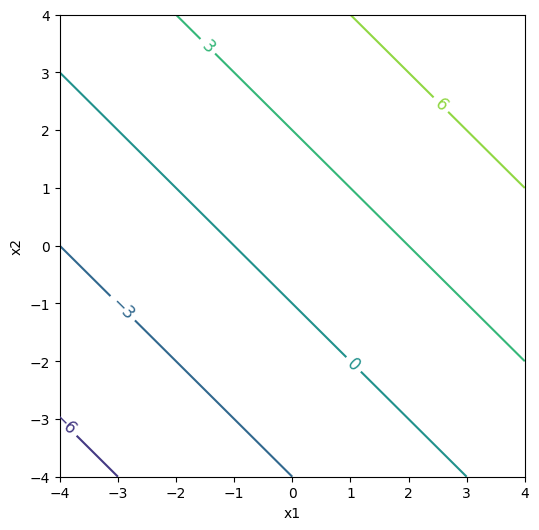
\includegraphics[width=\textwidth]{scaling1.png} 
        \caption{$f(x) = x_1 + x_2 + 1$} 
        \label{fig:original_scaled}
    \end{subfigure} 
    \hfill    
    \begin{subfigure}[b]{0.32\textwidth} 
        \centering 
        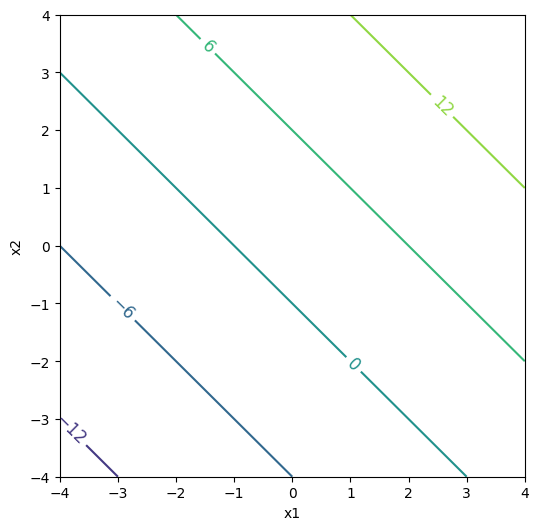
\includegraphics[width=\textwidth]{scaling2.png} 
        \caption{$f(x) = 2 x_1 + 2 x_2 + 2$} 
        \label{fig:two_times_scaled}
    \end{subfigure} 
    \hfill
    \begin{subfigure}[b]{0.32\textwidth} 
        \centering 
        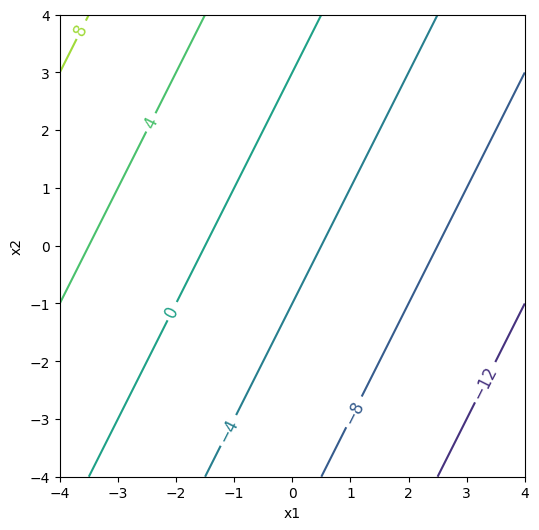
\includegraphics[width=\textwidth]{scaling3.png} 
        \caption{$f(x) = -2x_1 + x_2 - 3$} 
        \label{fig:something_else}
    \end{subfigure} 

    \caption{From (a), you can see that simply multiplying everything by two automatically increases our confidence by $2$, meaning that the functional margin can be scaled arbitrarily by scaing $(\mathbf{w}, b)$. There are still too many degrees of freedom in here and so extra constraints must be imposed. } 
    \label{fig:scaling_problem} 
\end{figure}


\subsection{Lagrange Duality} 

To minimize the equations with the constraint equations, we can use the method of Lagrange multipliers, which leads to to Lagrangian 
\[\mathcal{L}(\mathbf{w}, b, \boldsymbol{\alpha}) = \frac{1}{2} ||\mathbf{w}||^2 - \sum_i \alpha_i \big[ y_i (\mathbf{w} \cdot \mathbf{x}_i + b) - 1\big]\]
We can take the gradients with respect to $\mathbf{w}$ and $b$ and set them to $0$, which gives the two conditions 
\begin{align*} 
  \mathbf{w} & = \sum_i \alpha_i y_i \mathbf{x}_i \\
  0 & = \sum_i \alpha_i y_i \mathbf{x}_i 
\end{align*}

Now let's substitute our evaluated $\mathbf{w}$ back into $\mathcal{L}$, which gives the \textbf{dual representation} of the maximum margin problem in which we maximize  
\begin{align*} 
    L & = \frac{1}{2} \bigg( \sum_i \alpha_i y_i \mathbf{x}_i \bigg) \bigg( \sum_j \alpha_j y_j \mathbf{x}_j \bigg) - \sum_{i} \alpha_i y_i x_i \cdot \bigg[ \sum_j \alpha_j y_j x_j \bigg] - \sum_i \alpha_i y_i b + \sum_i \alpha_i \\ 
      & = \sum_i \alpha_i - \frac{1}{2} \sum_{i, j} \alpha_i \alpha_j y_i y_j \, \mathbf{x}_i \cdot \mathbf{x}_j 
\end{align*}
The summation with the $b$ in it is $0$ since we can pull the $b$ out and the remaining sum is $0$ from before. Now the optimization only depends on the dot product $\mathbf{x}_i \cdot \mathbf{x}_j$ of all pairs of sample vectors, which is very interesting. We will see more of this when we talk about kernel methods. Now, we need to solve the dual problem 
\[\max_{\boldsymbol{\alpha}} \mathcal{L}(\boldsymbol{\alpha})\]
which can be done using some generic quadratic programming solver or some other method to get the optimum $\boldsymbol{\alpha}^\ast$, which gives us 
\[\mathbf{w}^\ast = \sum_i \alpha_i^\ast y_i \mathbf{x}_i\]


\subsection{Nonseparable Case} 

\section{Naive Bayes}

Generative model. 




\section{Introduction}

\subsection{Bayesian Probability}

Now this book puts a heavy emphasis on Bayesian probabilistic models. For now, we will denote $p(X)$ to be the distribution of a random variable $X$. We capture our assumptions about the model parameter $\mathbf{w}$ with a prior distribution $p(\mathbf{w})$. Our likelihood $p(\mathcal{D} \mid \mathbf{w})$ is the conditional distribution of getting the data $\mathcal{D}$ from our model with parameter $\mathbf{w}$. Therefore, Bayes theorem is expressed 
\[p(\mathbf{w} \mid \mathcal{D}) = \frac{p(\mathcal{D} \mid \mathbf{w}) \, p(\mathbf{w})}{p(\mathcal{D})}\]
The denominator $p(\mathcal{D})$ is a normalizing term equal to $\int p(\mathcal{D} \mid \mathbf{w}) \, p(\mathbf{w}) \,d\mathbf{w}$, and for high dimensional $\mathcal{W}$ it may not be feasible to compute this integral without monte carlo sampling. Therefore, we focus on the numerator terms and remember the rule 
\[\text{posterior} \propto \text{likelihood} \times \text{prior}\]

For clarification, $\mathcal{D}$ can represent different things depending on the problem: 
\begin{enumerate}
    \item In a density estimation problem, where we have a single dataset $\mathbf{X}$, $\mathcal{D} = \mathbf{X}$ since this data tells us information about which distribution it could come from. 
    \item In a regression problem, $\mathcal{D} = \mathbf{Y}$, that is, $\mathcal{D}$ will always be the output data, not the input data $\mathbf{X}$. We can think of the input data $\mathbf{X}$ as always being fixed, and it is upon observation of the \textit{outputs} $\mathbf{Y}$ on these inputs that gives us information. 
\end{enumerate}

In both the frequentist and Bayesian settings, the likelihood $p(\mathcal{D} \mid \mathbf{w})$ plays a central role. In the frequentist setting, the process is divided into two steps: 
\begin{enumerate}
    \item We optimize $\mathbf{w}$ with some \textbf{estimator}, with a popular one being the \textbf{maximum likelihood estimator}. A popular estimator is \textbf{maximum likelihood}, which seeks to maximize $p(\mathcal{D} \mid \mathbf{w})$ w.r.t. $\mathbf{w}$. 
    \item We optimize $\mathbf{w}$ with some \textbf{estimator}, with a popular one being the \textbf{maximum likelihood estimator}. A popular estimator is \textbf{maximum likelihood}, which seeks to maximize $p(\mathcal{D} \mid \mathbf{w})$ w.r.t. $\mathbf{w}$. 
    \item We fix the optimized $\mathbf{w}^\ast$ and error bars on this estimate are obtained by considering the distribution of possible datasets $\mathcal{D}$. One approach is \textbf{bootstrapping}, which goes as follows. Given our original dataset $\mathbf{X} = \{x^{(1)}, \ldots, x^{(N)}\}$, we can create a new dataset $\mathbf{X}^\prime$ by sampling $N$ points at random from $\mathbf{X}$, with replacement, so that some points in $\mathbf{X}$ may be replicated in $\mathbf{X}^\prime$, whereas other points in $\mathbf{X}$ may be absent in $\mathbf{X}^\prime$. This process is repeated $L$ times to generate $L$ different datasets. Then, we can look at the variability of prediction between the different bootstrap data sets. 
\end{enumerate}
In a Bayesian setting, there is only a single dataset $\mathcal{D}$ and the uncertainity in the parameters is expressed through a probability distribution over $\mathbf{w}$. It also includes prior knowledge naturally in the form of prior distributions. 

\subsection{Density Estimation}

\subsubsection{Frequentist Approach}

As a start, let us have a dataset of observations $\mathbf{X} = \{x^{(1)}, \ldots, x^{(n)}\}$ assuming that they are all iid from $X \sim N(0, 1)$ distribution. Since this is iid, we can look at the joint distribution $X^N$ on $\mathbb{R}^N$ and get the likelihood of form
\[p(\mathbf{X} \mid \mu, \sigma^2) = \prod_{n=1}^N p_X (x^{(n)} \mid \mu, \sigma^2)\]
which in turn gives the log-likelihood as 
\[\ln p(\mathbf{X} \mid \mu, \sigma^2) = -\frac{1}{2 \sigma^2} \sum_{n=1}^N (x_n - \mu)^2 - \frac{N}{2} \ln \sigma^2 - \frac{N}{2} \ln(2 \pi)\]
This is a function of two variables, $\mu$ and $\sigma^2$ and we can optimize it to get the maximum likelihood estimates of 
\[\mu_{ML} = \frac{1}{N} \sum_{n=1}^N x_n \text{ and } \sigma^2_{ML} = \frac{1}{N} \sum_{n=1}^N (x_n - \mu_{ML})^2\]
However, as we saw in the previous section, the estimate for $\sigma^2$ is biased by a factor of $(N-1)/N$, and this is an intrinsic flaw in the frequentist approach. 

\subsubsection{Bayesian Approach}

In the Bayesian approach, we want to model
\[p(x \mid \mathcal{D}) = \int p(x \mid \mathbf{w}) \, p(\mathbf{w} \mid \mathcal{D}) \; d\mathbf{w}\]

\subsection{Regression with Regularization}

\subsubsection{Frequentist's Maximum Likelihood Approach}

Now given the hypothesis function $h_\mathbf{w}$, researchers assume that the relationship between the $X$ and $Y$ values are captured by 
\[Y = h_\mathbf{w}(X) + \epsilon\]
where $\epsilon$ is some residual noise, also a random variable. Researchers assume that this random variable has a nice form. One popular choice is that $\epsilon \sim N(0, \sigma^2)$ since if we assume that this error is due to a large number of weakly dependent unknown factors, then by CLT we can assume that their sum is Gaussian. But ultimately this is just another assumption. With this Gaussian assumption, we can assume that each input output pair $(x^{(n)}, y^{(n)})$ is generated by form $y^{(n)} = h_\mathbf{w} (x^{(n)}) + \epsilon$ and so the conditional distribution of $y^{(n)}$ given $X^{(n)}$ is 
\[Y \mid X = x^{(n)} \sim N( h_\mathbf{w} (x^{(n)}), \sigma^2) \]
and therefore, the probability of getting $y^{(n)}$ given $x^{(n)}$ is modeled by the conditional pdf 
\[p_{Y \mid X = x^{(n)}} (y^{(n)}) = \frac{1}{\sqrt{2 \pi \sigma^2}} \exp \bigg( -\frac{[ y^{(n)} - h_\mathbf{w} (x^{(n)}) ]^2}{2 \sigma^2} \bigg)\]
Extending this to the dataset $\mathcal{D} = \mathbf{Y}$ coming from the $N$-fold joint distribution of $X$, by independence this distribution is a multivariate Gaussian
\[Y^n \mid X^n = \mathbf{X} \sim N( h_\mathbf{w} (\mathbf{X}), \sigma^2 \mathbf{I})\]
where by abuse of notation, $h_\mathbf{w} (\mathbf{X})$ is $h_\mathbf{w}$ operated element-wise on the vector $\mathbf{X}$, and $\mathbf{I}$ is the $N \times N$ identity matrix. The pdf is 
\begin{align*}
    p_{Y^n \mid X^n = \mathbf{X}} (\mathbf{Y}) & = \prod_{n=1}^N p_{Y \mid X = x^{(n)}} (y^{(n)}) \\
    & = \prod_{n=1}^N \frac{1}{\sqrt{2 \pi \sigma^2}} \exp \bigg( -\frac{[ y^{(n)} - h_\mathbf{w} (x^{(n)}) ]^2}{2 \sigma^2} \bigg)
\end{align*}
The two parameters of interest here that we would like to maximize are $\mathbf{w}$ and $\sigma^2$. We can take the log of this function to maximize this, which gives us 
\[\ell(\mathbf{w}, \sigma^2) = -\frac{1}{\sigma^2} E_D (\mathbf{w}) - \frac{N}{2} \ln \sigma^2 - \frac{N}{2} \ln(2\pi)\]
and here we can see that maximizing the likelihood w.r.t. $\mathbf{w}$ is equal to minimizing the sum-of-squares error function $E_D(\mathbf{w}) = -\frac{1}{2} \sum_{n=1}^N [ y^{(n)} - h_\mathbf{w} (x^{(n)})]^2 $. Therefore, a maximum likelihood estimation under a Gaussian residual assumption implies minimization of the sum-of-squares error function! To maximize with respect to both $\mathbf{w}$ and $\sigma^2$, we can use the fact that this function is $C^1$ (continuously differentiable), and so we just need to find where the partials are $0$. Ultimately, we can just optimize for $\mathbf{w}$ first and then solve for $\sigma^2$. If $h_\mathbf{w}$ was linear (not necessarily in $\mathbf{x}$, but with $\mathbf{w}$), then we can transform the $x_d$ values, get the proper design matrix $\boldsymbol{\Phi}$, and compute 
\[\mathbf{w}_{ML} = (\boldsymbol{\Phi}^T \boldsymbol{\Phi})^{-1} \boldsymbol{\Phi}^T \mathbf{Y}\]
If we add a ridge penalty term to get $E(\mathbf{w}) = E_D (\mathbf{w}) + \frac{\lambda}{2} ||\mathbf{w}||^2_2$, then this results in solving the matrix equation
\[\mathbf{w}_{ML} = (\boldsymbol{\Phi}^T \boldsymbol{\Phi} + \lambda \mathbf{I})^{-1} \boldsymbol{\Phi}^T \mathbf{Y}\]
With these optimized parameters, we have a \textbf{probabilistic model} in which given a new value $\hat{\mathbf{x}}$, we can predict the conditional distribution of $\hat{y}$ to be 
\[p(y^\prime \mid \hat{\mathbf{x}}, \mathbf{w}_{ML}, \sigma^2_{ML}) = N(\hat{y} \mid h_{\mathbf{W}_{ML}} (\mathbf{x}^\prime), \sigma^2_{ML})\]

% Now, even if we choose precisely $g(X) = \mathbb{E}[Y \mid X]$, this will in most cases not be a perfect indicator of $Y$ since usually $\sigma(Y) \not\subset \sigma(X)$. Therefore, there is a \textbf{residual term} $\epsilon$ that is precisely the difference between $g(X)$ and $Y$. 
% \[Y = g(X) + \epsilon\]
% We do not know what this $\epsilon$ even is besides the fact that it does not live in the space of all $\sigma(X)$-measurable functions (since if it did, then it would be captured by $g$). We also know from the tower property that 
% \[\mathbb{E}[\epsilon] = \mathbb{E}[Y - \mathbb{E}[Y \mid X]] = \mathbb{E}[Y] - \mathbb{E}[Y] = 0\]


\subsubsection{Bayesian Approach}

We will now demonstrate how having a normal $\alpha \mathbf{I}$ prior around the origin in a Bayesian setting is equivalent to having a ridge penalty of $\lambda = \sigma^2 / \alpha^2$ in a frequentist setting. If we have a Gaussian prior of form 
\[p(\mathbf{w} \mid \alpha^2) = N(\mathbf{w} \mid \mathbf{0}, \alpha^2 \mathbf{I}) = \bigg( \frac{1}{2 \pi \alpha^2} \bigg)^{M/2} \exp \bigg( -\frac{1}{2\alpha^2} ||\mathbf{w}||^2_2 \bigg)\]
We can use Bayes rule to compute 
\begin{align*}
    p(\mathbf{w} \mid \mathbf{X}, \mathbf{Y}, \alpha^2, \sigma^2) & \propto p(\mathbf{Y} \mid \mathbf{w}, \mathbf{X}, \alpha^2, \sigma^2) \, p(\mathbf{w} \mid \mathbf{X}, \alpha^2, \sigma^2) \\
    & = \bigg[ \prod_{n=1}^N p(y^{(n)} \mid \mathbf{w}, \mathbf{x}^{(n)}, \alpha^2, \sigma^2 )\bigg] \, p(\mathbf{w} \mid \mathbf{X}, \alpha^2, \sigma^2) \\
    & = \bigg[ \prod_{n=1}^N \frac{1}{\sqrt{2 \pi \sigma^2}} \exp \bigg( - \frac{(y^{(n)} - h_\mathbf{w} (x^{(n)}))^2}{2 \sigma^2} \bigg) \bigg] \cdot \bigg( \frac{1}{2 \pi \alpha^2} \bigg)^{M/2} \exp \bigg( -\frac{1}{2\alpha^2} ||\mathbf{w}||^2_2 \bigg)
\end{align*}
and taking the negative logarithm gives us 
\[\ell(\mathbf{w}) = \frac{1}{2\sigma^2} \sum_{n=1}^N \big(y^{(n)} - h_\mathbf{w} (\mathbf{x}^{(n)}) \big)^2 + \frac{N}{2}\ln{\sigma^2} + \frac{N}{2} \ln(2\pi) - \frac{M}{2} \ln(2\pi \alpha^2) + \frac{1}{2 \alpha^2} ||\mathbf{w}||_2^2\]
taking out the constant terms relative to $\mathbf{w}$ and multiplying by $2 \sigma^2$ (which doesn't affect optima) gives us the ridge penalized error with a penalty term of $\lambda = \sigma^2 / \alpha^2$. 
\[E(\mathbf{w}) = \frac{1}{2} \sum_{n=1}^N \big(y^{(n)} - h_\mathbf{w} (\mathbf{x}^{(n)}) \big)^2 + \frac{\sigma^2}{\alpha^2} ||\mathbf{w}||_2^2\]
But minimizing this still gives a point estimate of $\mathbf{w}$, which is not the full Bayesian treatment. In a Bayesian setting, we are given the training data $(\mathbf{X}, \mathbf{Y})$ along with a new test point $\mathbf{x}^\prime$ and want to evaluate the predictive distribution $p(y \mid \mathbf{x}^\prime, \mathbf{X}, \mathbf{Y})$. We can do this by integrating over $\mathbf{w}$. 
\begin{align*}
    p(y \mid \mathbf{x}^\prime, \mathbf{X}, \mathbf{Y}) & = \int p(y \mid \mathbf{x}^\prime, \mathbf{w}, \mathbf{X}, \mathbf{Y}) \, p(\mathbf{w} \mid \mathbf{x}^\prime, \mathbf{X}, \mathbf{Y}) \, d \mathbf{w} \\
    & = \int p(y \mid \mathbf{x}^\prime, \mathbf{w}) \, p(\mathbf{w} \mid \mathbf{X}, \mathbf{Y}) \, d \mathbf{w} 
\end{align*}
where we have omitted the irrelevant variables, along with $\alpha^2$ and $\sigma^2$ to simplify notation. By substituting the posterior $p(\mathbf{w} \mid \mathbf{X}, \mathbf{Y})$ with a normalized version of our calculation above and by noting that 
\[p(y \mid \mathbf{x}^\prime, \mathbf{w}) = N(y \mid h_\mathbf{w} (\mathbf{x}^\prime), \sigma^2) = \frac{1}{\sqrt{2 \pi \sigma^2}} \exp \bigg( -\frac{\big(y - h_\mathbf{w} (\mathbf{x}^\prime)\big)^2}{2 \sigma^2} \bigg)\]
Now this integral may or may not have a closed form, but if we consider the polynomial regression with the hypothesis function of form 
\[h_\mathbf{w} (x) = w_0 + w_1 x + w_2 x^2 + \ldots + w_{M-1} x^{M-1}\]
then this integral turns out to have a closed form solution given by 
\[p(y \mid \mathbf{x}^\prime, \mathbf{X}, \mathbf{Y}) = N \big( y \mid m(x^\prime), s^2 (x^\prime)\big)\]
where 
\begin{align*}
    m(x^\prime) & = \frac{1}{\sigma^2} \boldsymbol{\phi}(x^\prime)^T \mathbf{S} \bigg( \sum_{n=1}^N \boldsymbol{\phi}(x^{(n)}) y^{(n)} \bigg) \\
    s^2 (x^\prime) & = \sigma^2 + \boldsymbol{\phi}(x^\prime)^T \mathbf{S} \boldsymbol{\phi}(x^\prime) \\
    \mathbf{S}^{-1} & = \alpha^{-2} \mathbf{I} + \frac{1}{\sigma^2} \sum_{n=1}^N \boldsymbol{\phi}(x^{(n)}) \boldsymbol{\phi}(x^\prime)^T 
\end{align*}
and $\boldsymbol{\phi}(x)$ is the vector of functions $\phi_i (x) = x^i$ from $i = 0, \ldots, M-1$. 

\end{document}
